% !TEX root = LF-IMAPol.tex

\chapter{Lexical networks}\label{chap:lexicalNetwork}

This concluding chapter examines the role played by lexical functions [LFs] in the structure of natural language lexicons and, consequently, their relevance to the structuring of lexicon models\index[notion]{lexicon!structure of the \tld}. Because lexicons are large informational systems involved in complex mental processes (speech production\slashs{}understanding\index[notion]{speech!\tld\ production}\index[notion]{speech!\tld\ understanding}, language acquisition\index[notion]{acquisition!language \tld}, reasoning with elaborate concepts, etc.), they can be expected to have a structure that supports their involvement in such processes, and it is there that LFs come into play.

The preceding chapters deal with the relevance of LFs from a dual perspective:

\begin{itemize}

\item writing lexical entries\index[notion]{lexical entry} -- cf. the cooccurrence zone\index[notion]{lexical entry!cooccurence zone of a \tld}\index[notion]{zone of a lexical entry!cooccurrence \tld} of corresponding lexical entries, as illustrated with the entry for \textsc{anger}\tsub{(N)} (Appendix, p.\thinspace\pageref{chap:appendix1});\footnote{LF applications that systematically illustrate the presentation of each individual LFs in Chapters~\ref{chap:paraLFs} and~\ref{chap:syntLFs} are in reality part of lexicographic information: an expression of the form ``\lfappl{f}{L}~=~L′\thinspace'' belongs to the cooccurrence zone of L's lexical entry.}

\item modeling lexical selection\index[notion]{lexical selection} in speech production\index[notion]{speech!\tld\ production} (\chapref{chap:NotionLF}, \sectref{sec:LFAndLexicalization}) -- cf. the role of LFs in deep-syntactic structures\index[notion]{structure!deep-syntactic \tld\ [DSyntS]}\index[notion]{deep-syntactic!\tld\ structure [DSyntS]}\index[notion]{syntax!deep \tld} and in deep-syntactic paraphrasing rules\index[notion]{paraphrase!deep-syntactic paraphrasing rule} described throughout the book.

\end{itemize}

We now take a broader view of the system of standard LFs\index[notion]{system of standard LFs} and explain the key role they play in organizing the Speaker's \notion{lexical knowledge}\index[notion]{lexical knowledge|emph}. The implication of what will be presented now is twofold.

First, the system of lexical relations induced by LF applications\index[notion]{application of an LF}\index[notion]{lexical function!application of a \tld} can be used to determine the shape of new \notion{models of the lexicon} -- for short, \notion{lexicon models}\index[notion]{model!lexicon \tld}\index[notion]{lexicon!\tld\ model} -- and, therefore, can be exploited to develop a new type of lexicography\index[notion]{lexicography} that goes beyond traditional dictionary\index[notion]{dictionary} writing (as demonstrated in \sectref{sec:fr-LN}, p.\thinspace\pageref{sec:fr-LN}).

Second, in terms of applicability, lexicon models primarily structured by LF relations are expected to be better \notion{data structures}\index[notion]{data structure}\index[notion]{structure!data \tld} than ordinary -- textual -- dictionaries, in the sense that they are better tools for the study and description of essential lexicon-related phenomena, such as lexical acquisition\index[notion]{acquisition!lexical \tld} and lexical access\slashs{}selection\index[notion]{lexical access\slashs{}selection} by the Speaker.

The present chapter contains the following sections:

\begin{itemize}

\item \nameref*{sec:shapeOfLexicons} (\sectref{sec:shapeOfLexicons})

\item \nameref*{sec:LexicalSystems} (\sectref{sec:LexicalSystems})

\item \nameref*{sec:fr-LN} (\sectref{sec:fr-LN})

\end{itemize}


\section{What is the ``shape'' of natural language lexicons?}\label{sec:shapeOfLexicons}

The question of the structure of lexical knowledge -- and, consequently, the formal structure of models that describe it -- has been largely disregarded by lexicologists and lexicographers in favor of a dictionary-based\index[notion]{dictionary} approach. Under this approach, the \notion{macrostructure}\index[notion]{dictionary!macrostructure of a \tld}\index[notion]{macrostructure (of a dictionary)} \parencite{Wiegand1996} of a lexicon model\index[notion]{lexicon!\tld\ model}\index[notion]{model!lexicon \tld} is an alphabetically sorted list of lexical entries; this is the common way to structure most of the known dictionaries. However, there have been notable exceptions, for instance:

\begin{itemize}

\item For dictionaries: \notion{production dictionaries}\index[notion]{dictionary!production \tld}, inaugurated for English by the \textit{Longman Language Activator}\index[notion]{Longman Language Activator@\textit{Longman Language Activator}}\index[notion]{dictionary!Longman Language Activator@\textit{Longman Language Activator}} \parencite{LongmanActivator1993}. Its thesaurus-like macrostructure gives the users access to lexical entries\index[notion]{lexical entry} via a set of conceptual keywords, thus breaking the linear alphabetical barrier and allowing for a semantic navigation through lexical knowledge.\footnote{Cf. the illustration given in \textcite[176]{RundellHam1994}: the ANGRY concept, which gives access to (dictionnary entries for) lexical realizations such as: \textit{angry}, \textit{cross}, \textit{enrage}, \textit{fly off the handle}, \textit{furious}, \textit{incensed}, \textit{mad}, \textit{maddening}, \textit{mollify}, \textit{rage}, \textit{stormy}, \textit{wind someone up}.}

\item For lexical databases\index[notion]{lexical database}: \notion{\textit{-Net} models}\index[notion]{model!-Net@\textit{-Net} \tld|emph}\index[notion]{net@\textit{-Net} model|emph} \parencite{Fontenelle2012}, such as the family of \mbox{\notion{WordNets}}\index[notion]{lexical database!WordNet} (Princeton WordNet\index[notion]{WordNet!Princeton \tld}, EuroWordNet\index[notion]{WordNet!Euro\tld}, etc.), which adopt a \notion{taxonomic}\index[notion]{taxonomy}\index[notion]{lexical network!taxonomic \tld} perspective on the structuring of lexical knowledge \parencite{Fellbaum1998}, or \notion{FrameNet}\index[notion]{FrameNet}\index[notion]{lexical database!FrameNet}, which is based on lexical relations induced by Frame Semantics\index[notion]{Frame Semantics} \parencite{FillmoreEtAl2003}.

\end{itemize}

Given this state of affairs, we have to answer the following question: What is the ``shape'' of a natural language lexicon? Of course, a real lexicon of natural language is a purely informational (non-physical) entity and does not have actual physical shape. We use the figurative expression \textit{shape of the lexicon} in order to stress the fact that, in advanced formal lexicology and lexicography, we need adequate structuring and visualizations\index[notion]{visualization} of lexicon models\index[notion]{lexicon!\tld\ model}\index[notion]{model!lexicon \tld} (see \figref{fig:taxonomicNonTaxonomicLNs}, p.\thinspace\pageref{fig:taxonomicNonTaxonomicLNs}) that could support reasoning on such knowledge representations.

To develop the notion of lexicon model, we will introduce two postulates: one immediately below and the second in \sectref{sec:LexicalSystems} (p.\thinspace\pageref{txt:postulateStrucLS}).

\phantomsection\label{txt:postulateStrucLexicons}\begin{soundbox}{Postulate 1: structure of lexicons}
Natural language lexicons are, first and foremost, sets of lexical entities\index[notion]{lexical entity} connected by lexical relations\index[notion]{lexical relation}\index[notion]{relation!lexical \tld}. Formally, they are \notion{lexical networks}\index[notion]{lexical network|emph}\index[notion]{network \lfgp{see also \textit{graph}}!lexical \tld|emph}; therefore, lexicon models\index[notion]{lexicon!\tld\ model}\index[notion]{model!lexicon \tld} should be structured as lexical networks.
\end{soundbox}

This postulate is taken for granted  -- by definition, a postulate does not call for a proof. However, its \emph{adequacy} can be evaluated in the context of descriptive lexicology\index[notion]{lexicology} -- i.e., lexicography\index[notion]{lexicography} -- and in that of its applications -- language teaching\index[notion]{teaching\slashs{}learning, language}\index[notion]{language teaching\slashs{}learning}, Natural Language Processing\index[notion]{Natural Language Processing}, etc. Postulate~1 is also in line with a whole array of observations made in disciplines as varied as psycholinguistics\index[notion]{psycholinguistics}, speech disorder\index[notion]{speech!\tld\ disorder} research or neurolinguistics\index[notion]{neurolinguistics}.\footnote{This is no place for a detailed review of the huge literature on the application of lexical networks in these areas. We content ourselves with the mention of particularly significant texts.}

Lexical networks are often associated in contemporary research with the notion of \notion{Mental Lexicon}\index[notion]{lexicon!Mental Lexicon}\index[notion]{Mental Lexicon} -- roughly, lexical knowledge as stored in the brain \parencite{Aitchison2012,DeDeyneEtAl2017}.
We believe that network models of the lexicon are indeed plausible models of the Mental Lexicon or, to put it more broadly, of the lexicon in its ``cognitive reality'' \parencite[Sec.~6]{GoddardForthcoming}.

\largerpage[2]
Mere adherence to the principle of representing lexical knowledge as lexical network is insufficient to properly determine the formal nature of resulting lexicon models. The lexicon is a set of lexical entities, but which ones? They are connected by relations, but which ones? The nature of these entities and these relations determines the actual formal structure of lexicon models. To illustrate this, let us contrast two approaches to structuring lexical networks: taxonomic networks, exemplified with the Princeton WordNet, vs. small-world networks, exemplified with the French Lexical Network [fr-LN], presented in \sectref{sec:fr-LN} (p.\thinspace\pageref{sec:fr-LN}).

The Princeton WordNet\index[notion]{WordNet!Princeton \tld|emph}\index[notion]{lexical database!WordNet|emph} for English\footnote{We focus here on the Princeton WordNet for the English language. The WordNet approach has been applied to a broad range of natural languages and has also been adapted to the construction of multilingual lexical resources \parencite{FellbaumVossen2012}.} is a computational lexicon model -- a lexical database -- that follows taxonomic principles\index[notion]{taxonomy|emph}\index[notion]{lexical network!taxonomic \tld|emph} postulated in the context of psycholinguistic\index[notion]{psycholinguistics} research \parencite{MillerEtAl1990}.\footnote{A taxonomy -- in the most general sense -- is a model of a vast natural domain organized as a hierarchy of classes and subclasses of entities. Linnaeus's classification of species is generally cited as prototypical taxonomic model in science. For a presentation and critique of this taxonomy, see \textcite{Ereshefsky1994}.} It is probably the most well\pagebreak-known and most widely used lexical database in Natural Language Processing\index[notion]{Natural Language Processing}. In the Princeton WordNet, lexical units, called \textit{senses}, are grouped into small sets of \mbox{(quasi-)}synonyms, called \textit{synsets}, and it is those synsets that are linked within the original WordNet's lexical network. They constitute lexical classes\index[notion]{class, lexical} primarily connected by the relation of hyperonymy\slashs{}hyponymy\index[notion]{lexical relation}\index[notion]{relation!lexical \tld}\index[notion]{hyperonymy/hyponymy@hyperonymy\slashs{}hyponymy}. This entails a global taxonomic organization of the lexicon model, characterized by its creators as being an \textit{inheritance system}\index[notion]{inheritance!\tld\ system} \parencite[242]{MillerEtAl1990}.

The fr-LN\index[notion]{French Lexical Network [fr-LN]}\index[notion]{lexical network!French \tld\ [fr-LN]}\index[notion]{lexical database!French Lexical Network [fr-LN]} \parencite{LuxPogodallaPolguere2011} is a computational lexicon model built according to the principles of Explanatory Combinatorial Lexicology\index[notion]{lexicology!Explanatory Combinatorial \tld}\index[notion]{Explanatory Combinatorial!\tld\ Lexicology}. Its structure has the characteristic properties of small-world networks\index[notion]{lexical network}\index[notion]{small-world!\tld\ network}\index[notion]{network \lfgp{see also \textit{graph}}!small-world \tld}\index[notion]{lexical network!small-world \tld} (see details in Sections~\ref{sec:LexicalSystems} and \ref{sec:fr-LN}); it can be loosely characterized as being a ``social network'' of lexical entities (mainly, lexical units) connected by paradigmatic and syntagmatic lexical relations, that are, in most part, LF relations. Though not taxonomic, its small-world organization puts order in the apparent mess of the lexicon: this organization allows for the computation of meaningful lexical clusters\index[notion]{cluster of nodes in a graph!lexical \tld}\index[notion]{node of a network\slashs{}graph!cluster of \tlds} and, more generally, of topological proximity\index[notion]{proximity, lexical}\index[notion]{topology!topological proximity}\index[notion]{graph!topology of a \tld}.\footnote{On the topological proximity of lexical nodes in networks\slashs{}graphs, see \sectref{sec:lexicalProximityTopologicalProximity}, p.\thinspace\pageref{sec:lexicalProximityTopologicalProximity}.}

\figref{fig:taxonomicNonTaxonomicLNs} visualizes the formal gap between the two approaches; it features:

\begin{itemize}
\item a sample of WordNet's taxonomy\index[notion]{taxonomy} centered around the lexical unit \textsc{watercourse}\sensenum{2} -- a member of the ``\{\thinspace\textsc{stream}\sensenum{1}, \textsc{watercourse}\sensenum{2}\thinspace\}'' \textit{synset};
\item a sample of the fr-LN centered around the corresponding French lexical unit \idiom{\textsc{cours d'eau}}, where the geometric distribution\index[notion]{node of a network\slashs{}graph!geometric distribution of \tlds}\index[notion]{geometric distribution of graph nodes} of lexical nodes reflects their topological proximity in the lexical network.
\end{itemize}

\begin{figure}

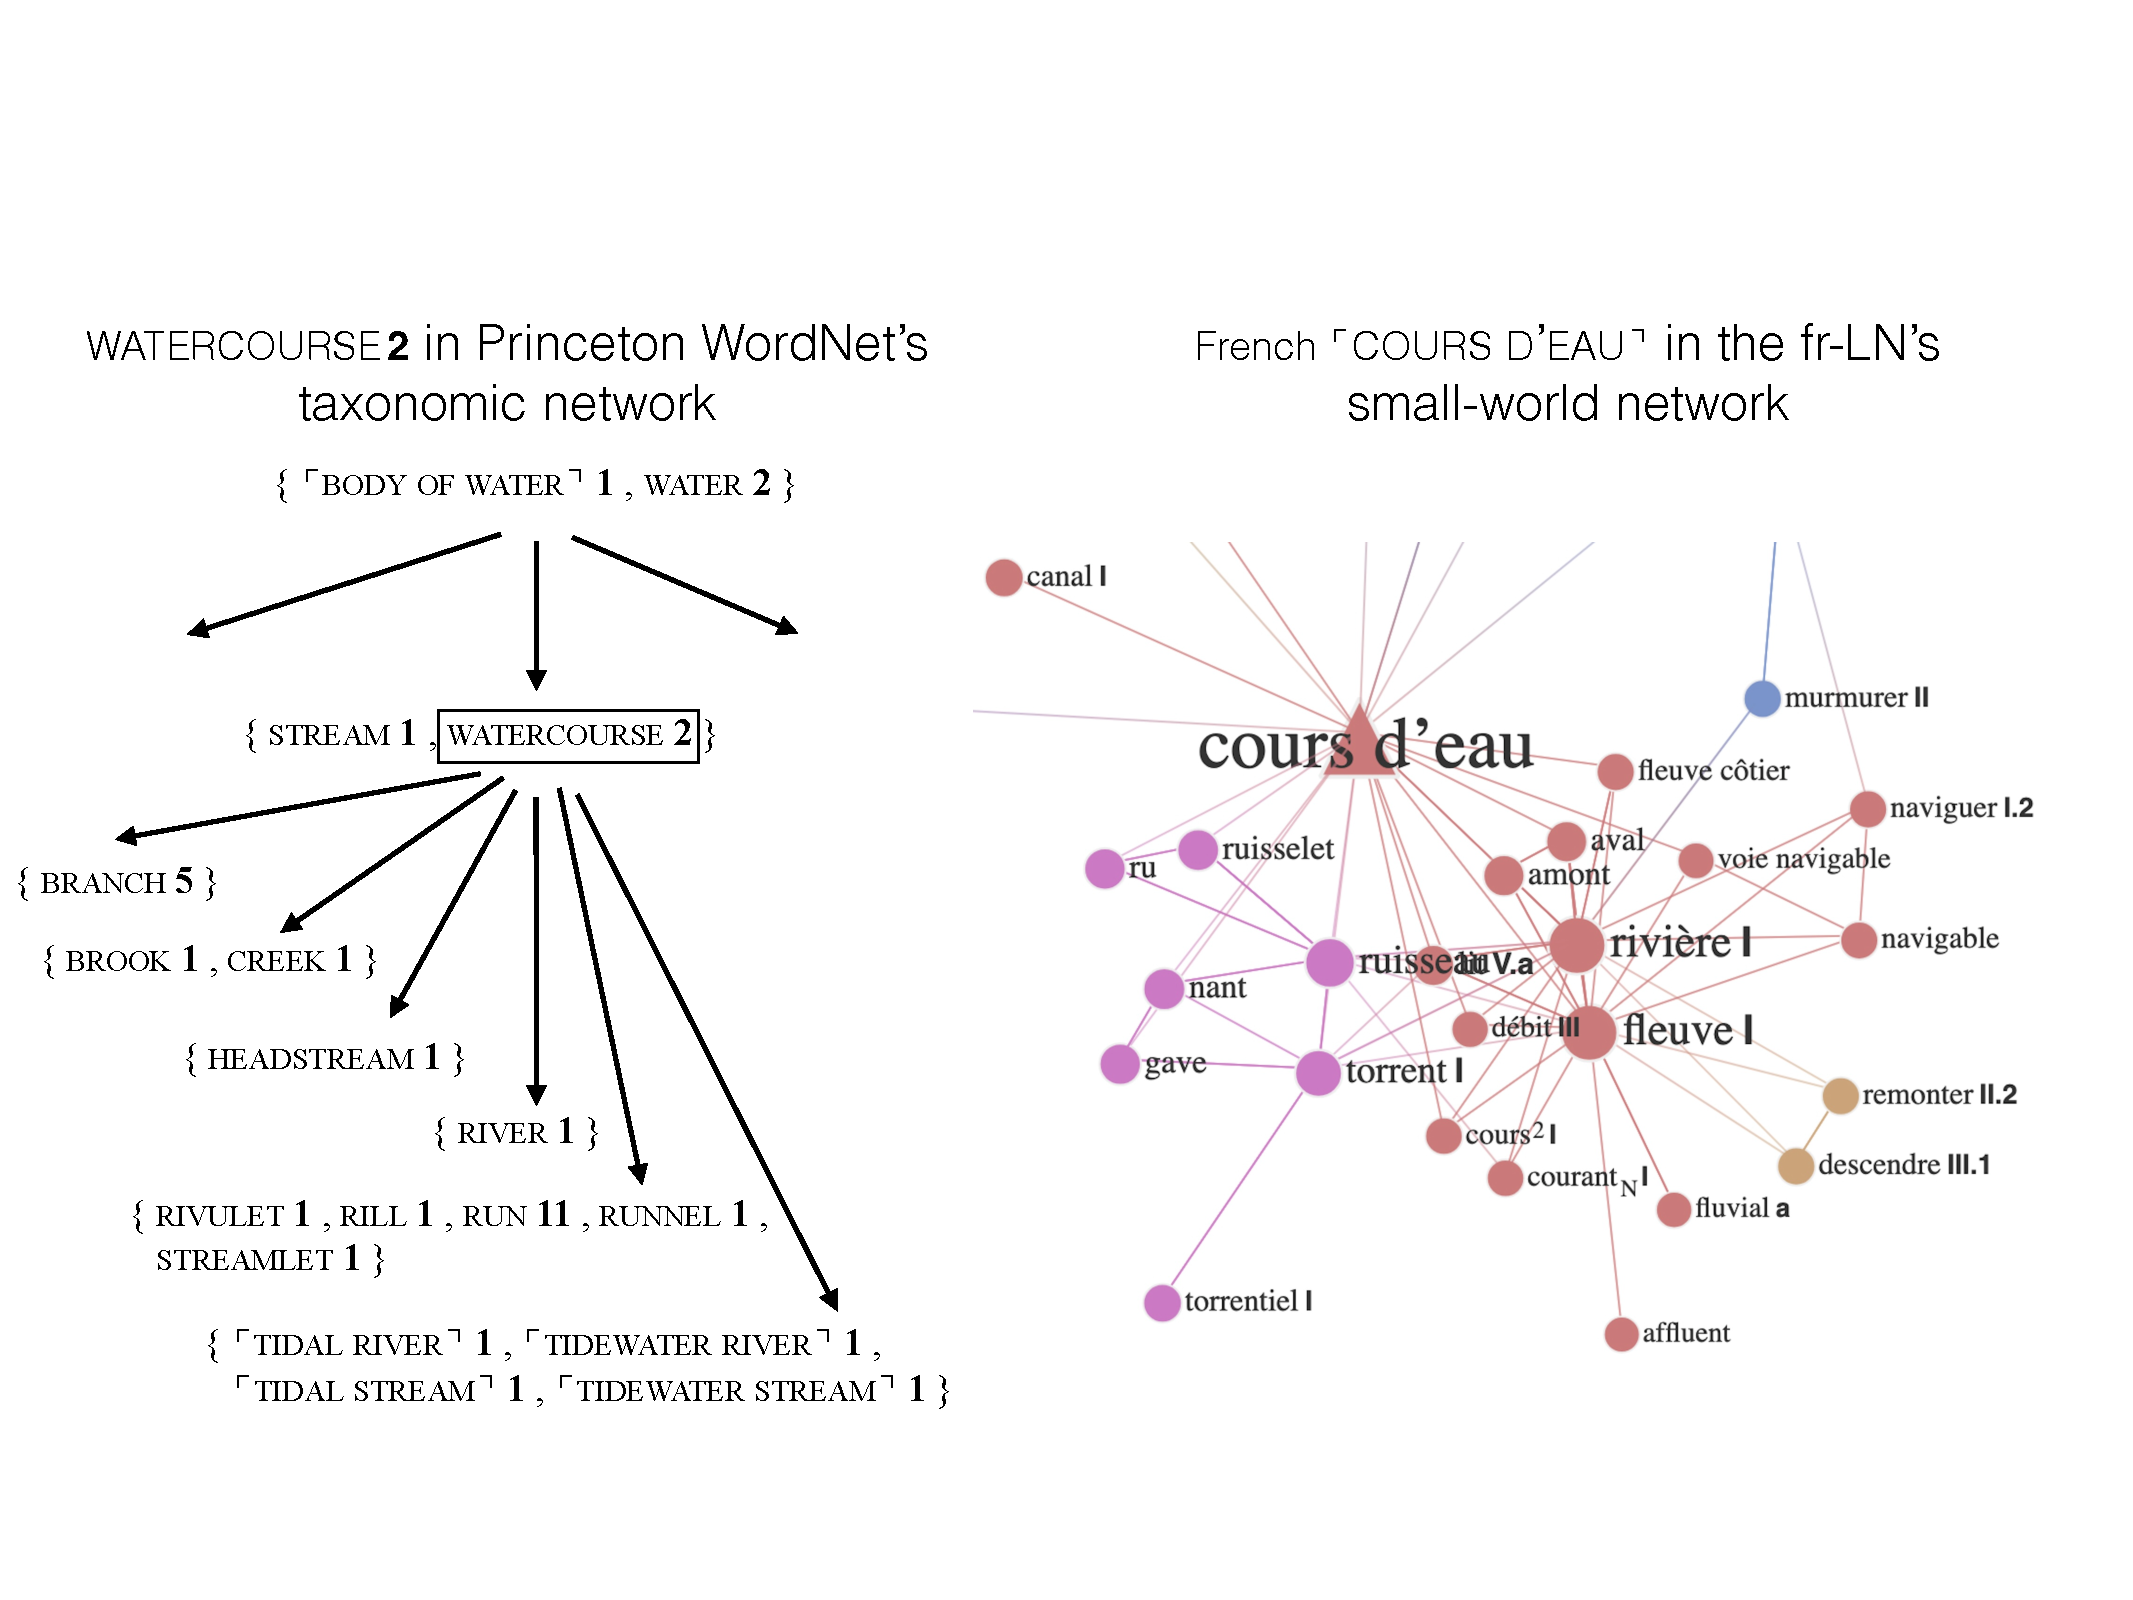
\includegraphics[width=0.97\linewidth]{Fig/LexicalNetworks/TaxonomicSmallworldLN.pdf}
\caption{Taxonomic vs. small-world lexical networks}\label{fig:taxonomicNonTaxonomicLNs}
\end{figure}

Though both the Princeton WordNet and the fr-LN have the ambition to reflect the organization of the Mental Lexicon, \figref{fig:taxonomicNonTaxonomicLNs} clearly shows how different structuring principles adopted for lexical network models induce different characteristic ``shapes'' of these models.\footnote{For arguments in favor of choosing small-world lexical networks over taxonomic ones, see \textcite{Polguere2014c-e} and \textcite{GotkovaEtAl2024}. The computable nature of small-world lexical networks as data structures is presented in \sectref{sec:formalPropertiesLS} (p.\thinspace\pageref{sec:formalPropertiesLS}).}\index[notion]{data structure}\index[notion]{structure!data \tld}

We present in \sectref{sec:LexicalSystems} (p.\thinspace\pageref{sec:LexicalSystems}) lexicon models called Lexical Systems\index[notion]{Lexical System}, of which the fr-LN is a particular instance, and highlight the fundamental role played by LF relations in such network lexicon models. Before we do that, let us briefly examine paradigmatic lexical relations encoded in WordNet from the perspective of LFs.

\paragraph*{WordNet's paradigmatic relations from the LF perspective.}\label{par:paraRelWordNet}

The taxonomic organization of WordNet -- illustrated in \figref{fig:taxonomicNonTaxonomicLNs} -- operates only in the nominal component of this lexical database\index[notion]{lexical database!WordNet}\index[notion]{WordNet!Princeton \tld} \parencite{Miller1990}, which is subdivided according to part of speech classification (nouns, verbs, adjectives and adverbs) and follows different structuring principles for each part of speech.

Furthermore, WordNet has a hybrid network structure where \textit{senses} themselves (and not only \textit{synsets}) can be connected. Such is the case for WordNet's so-called \textit{morphosemantic links}, which were grafted onto the original version of the database \parencite{MillerFellbaum2003}: they indicate lexical relations that would be encoded by us with paradigmatic LFs\index[notion]{lexical function!paradigmatic \tld}\index[notion]{paradigmatic!\tld\ lexical function}. In WordNet, these links are not typed, but identified under the same label: \texttt{derivation}, described as being a ``derivational morphology pointer.'' This is illustrated in \figref{fig:subnetworkWordNetMARRY-1}, which shows the WordNet subnetwork of \texttt{derivation} links extracted by taking the sense \textsc{marry}\sensenum{1} as point of origin and recursively following these links until all available \texttt{derivation} links are exhausted.\footnote{The present discussion is based on data extracted from version 3.1 of the Princeton WordNet.}

In order to clarify the nature of WordNet senses appearing in \figref{fig:subnetworkWordNetMARRY-1}, we list in 	\tabref{tab:ExtractWNPolysemyMARRY} their definitions in WordNet -- called \textit{glosses}\index[notion]{gloss in WordNet}\index[notion]{WordNet!gloss of a \tld\ sense} \parencite[240]{MillerEtAl1990} -- together with the relevant neighboring polysemy\index[notion]{polysemy}.

\begin{figure}

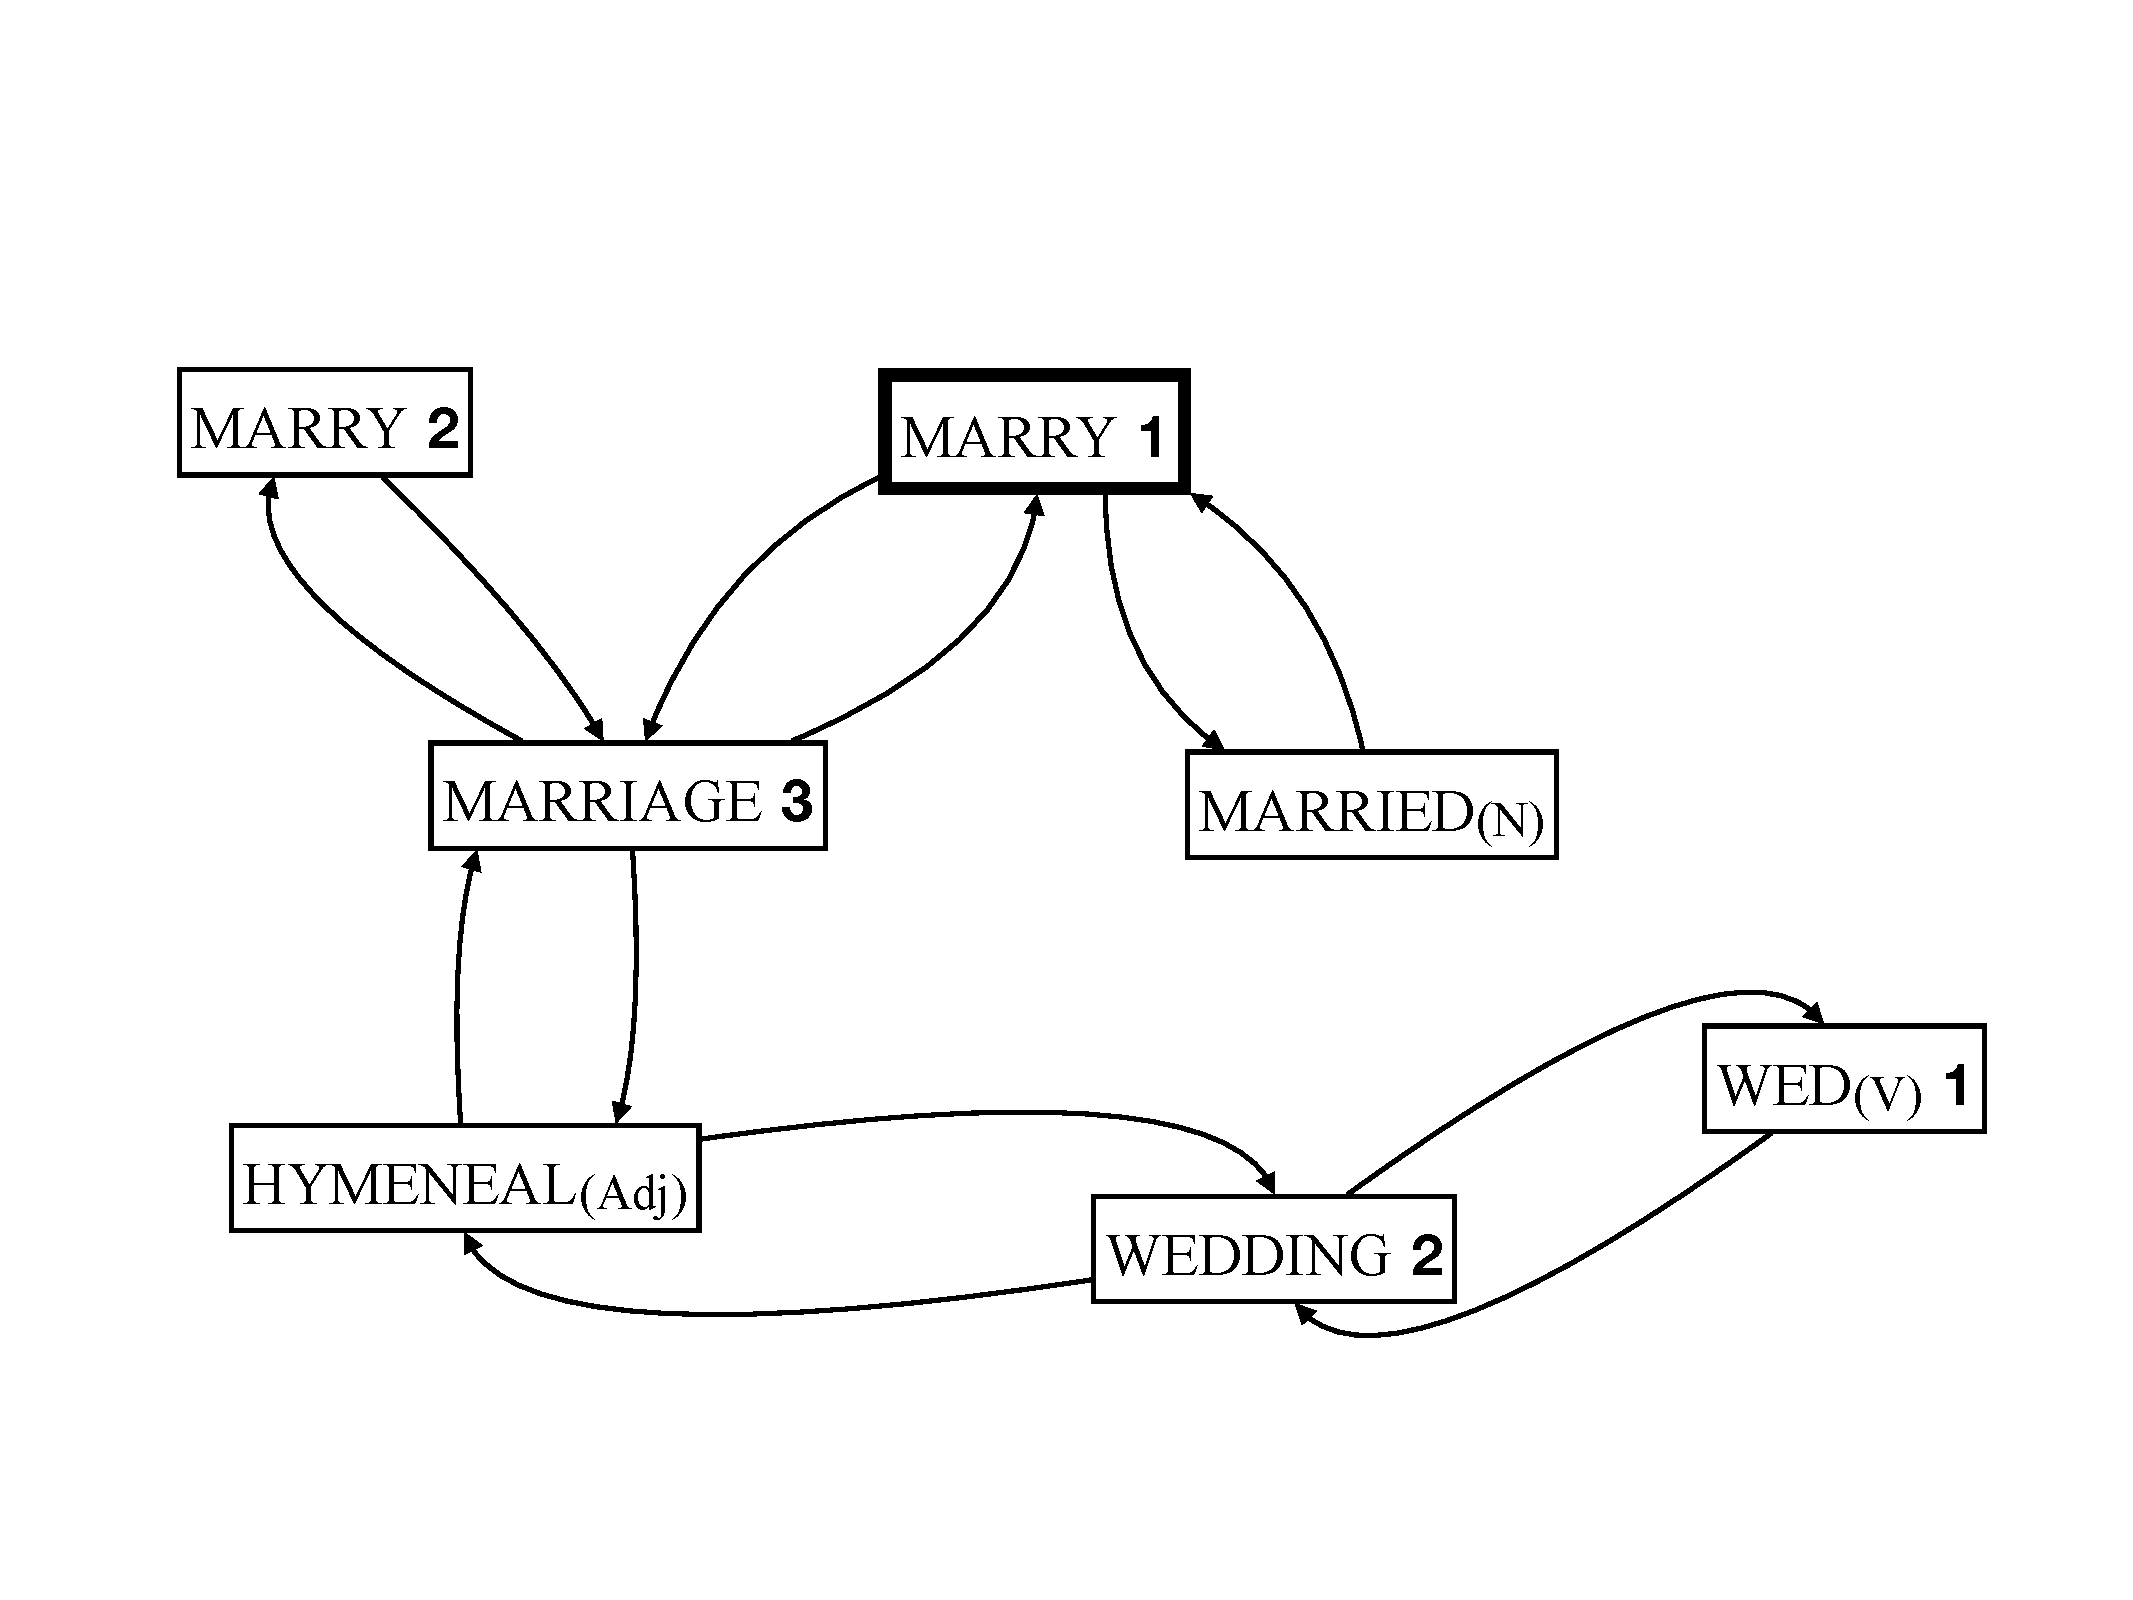
\includegraphics[width=.53\linewidth]{Fig/LexicalNetworks/subnetworkWordNetMARRY-1.pdf}
\caption{Subnetwork of \texttt{derivation} links in WordNet originating from \textsc{marry}\sensenum{1}}\label{fig:subnetworkWordNetMARRY-1}
\end{figure}

\begin{table}

\footnotesize
\renewcommand*{\arraystretch}{1}
\setlength{\tabcolsep}{4pt}
\begin{tabular}{ >{\raggedright\arraybackslash}p{.15\linewidth}  >{\raggedright\arraybackslash}p{.80\linewidth} }
\lsptoprule

\textsf{Senses}
& \textsf{Glosses} \\
\midrule

\lu{marry}{}{}{1}
& \textit{take in marriage} \\
\lu{marry}{}{}{2}
& \textit{perform a marriage ceremony} \\

\midrule

\lu{marriage}{}{}{1}
& \textit{the state of being a married couple voluntarily joined for life (or until divorce)} \\
\lu{marriage}{}{}{2}
& \textit{two people who are married to each other} \\
\lu{marriage}{}{}{3}
& \textit{the act of marrying; the nuptial ceremony} \\

\midrule

\lu{married}{(N)}{}{}
& \textit{a person who is married} \\

\midrule

\lu{hymeneal}{(Adj)}{}{}
& \textit{of or relating to a wedding or marriage} \\

\midrule

\lu{wedding}{}{}{1}
& \textit{the social event at which the ceremony of marriage is performed} \\
\lu{wedding}{}{}{2}
& same gloss as its synonym \lu{marriage}{}{}{3}: it belongs to the same synset (WordNet's glosses are associated to synsets, not to individual senses) \\

\midrule

\lu{wed}{(V)}{}{1}
& same gloss as its synonym \lu{marry}{}{}{1} \\
\lu{wed}{(V)}{}{2}
& same gloss as its synonym \lu{marry}{}{}{2} \\

\lspbottomrule
\end{tabular}\caption{Extract of WordNet's polysemy around the vocable \textsc{marry}}\label{tab:ExtractWNPolysemyMARRY}
\end{table}

Let us make three comments about \figref{fig:subnetworkWordNetMARRY-1}, taking the perspective of the encoding of paradigmatic relations by means of LFs.

\begin{enumerate}

\item WordNet's \texttt{derivation} links encode a very heterogeneous set of paradigmatic relations that can be discriminated with LFs; e.g., in \figref{fig:subnetworkWordNetMARRY-1}:

\begingroup
\small

\ex. \begingroup\setlength{\tabcolsep}{2pt}
\begin{tabular}[t]{ >{\raggedright\arraybackslash}p{2cm} >{\raggedright\arraybackslash}p{2cm} >{\raggedright\arraybackslash}p{6cm} }
\lu{marry}{}{}{1} & \lexRel{\lf{S\tsub{0}}} & \lu{marriage}{}{}{3}\\
\lu{marriage}{}{}{3} & \lexRel{\lf{V\tsub{0}}} & \lu{marry}{}{}{1}\\
\lu{marry}{}{}{1} & \lexRel{\lf{S\tsub{1/2}Perf}} & \lu{married}{(N)}{}{}\\
\end{tabular}\endgroup

\endgroup

This is a known issue with \texttt{derivation} links in WordNet. For a proposal to improve the description, see \textcite{FellbaumEtAl2009}.

\item A \texttt{derivation} link does not necessarily encode a morphological derivation\index[notion]{morphology!morphological derivative}\index[notion]{derivative!morphological \tld}, in spite of being termed \textit{morphosemantic} in the WordNet literature. Such is the case of the link between \lu{marriage}{}{}{3} and \lu{hymeneal}{(Adj)}{}{} in \figref{fig:subnetworkWordNetMARRY-1}: a case of \lf{A\tsub{0}}, in terms of LFs. Because morphology is not necessarily involved, these links can be considered as encoding \emph{semantic} derivations\index[notion]{semantic!\tld\ derivative}\index[notion]{derivative!semantic \tld}, just like paradigmatic LFs.

\item The encoding of semantic derivations in WordNet can be implemented in surprising ways. For instance, the absence of \textsc{spouse} in \figref{fig:subnetworkWordNetMARRY-1} is somehow strange, given the presence of the very marginal term \textsc{married}\tsub{(N)}. The noun \textsc{spouse} happens to be connected to \lu{marriage}{}{}{2} -- not \lu{marriage}{}{}{3} -- by the WordNet relation of meronymy\index[notion]{meronymy}. Because \lu{marriage}{}{}{2} is glossed as denoting a set of two persons rather than a social relation between two individuals (cf. 	\tabref{tab:ExtractWNPolysemyMARRY}),\footnote{WordNet illustrates this sense with the following example: \textit{his second marriage was happier than the first}.} \textsc{spouse} is modeled as denoting a unit of a marriage\sensenum{2} and therefore does not surface in \figref{fig:subnetworkWordNetMARRY-1}.

\end{enumerate}

This last observation illustrates the importance of organizing the modeling of paradigmatic -- and syntagmatic! -- relations by means of a coherent, well-defined \emph{system} of such relations that guides the process of exploring -- not just encoding -- lexical relations.

\section{Lexical Systems as network lexicon models}\label{sec:LexicalSystems}

A \notion{Lexical System}\index[notion]{Lexical System|emph} \parencite{Polguere2009-e,Polguere2014c-e} -- with capitalized initials -- is a lexicon model structured as a network of lexical entities connected, primarily, by paradigmatic and syntagmatic LF relations. Though built according to the principles of Explanatory Combinatorial Lexicology\index[notion]{Explanatory Combinatorial!\tld\ Lexicology}\index[notion]{lexicology!Explanatory Combinatorial \tld}, Lexical Systems have a formal structure radically different from that of Explanatory Combinatorial Dictionaries\index[notion]{Explanatory Combinatorial!\tld\ Dictionary}\index[notion]{dictionary!Explanatory Combinatorial \tld} \parencite{MelcukZholkovsky1984,MelcukZolkovskij2016,MelcukEtAl1984,MelcukEtAl1988,MelcukEtAl1992,MelcukEtAl1999}, these latter being textual (therefore, linear) representations of lexical knowledge\index[notion]{lexical knowledge}.

This section contains two parts: main characteristics of Lexical Systems (\sectref{sec:mainCharacteristicsLS}) and formal properties of Lexical Systems (\sectref{sec:formalPropertiesLS}).

The Lexical System approach has been applied to the construction of several lexical networks (LNs), in particular, for French (fr-LN)\index[notion]{French Lexical Network [fr-LN]}\index[notion]{lexical network!French \tld\ [fr-LN]}\index[notion]{lexical database!French Lexical Network [fr-LN]}, English (en-LN)\index[notion]{English Lexical Network [en-LN]}\index[notion]{lexical network!English \tld\ [en-LN]}\index[notion]{lexical database!English Lexical Network [en-LN]} and Russian (ru-LN)\index[notion]{Russian Lexical Network [ru-LN]}\index[notion]{lexical network!Russian \tld\ [ru-LN]}\index[notion]{lexical database!Russian Lexical Network [ru-LN]}. Because at the present time only the fr-LN (\sectref{sec:fr-LN}) can be considered as being a full-fledged Lexical System, our illustrations are mostly borrowed from this particular lexical database.\footnote{For information on exploratory lexicographic work conducted on the en-LN, see \textcite{GaderEtAl2014a-e}; on the ru-LN, see \textcite{Krylosova2017-e} and \textcite{Mikhel2022b}.}

\subsection{Main characteristics of Lexical Systems}\label{sec:mainCharacteristicsLS}

\subsubsection{LF relations: the backbone of Lexical Systems}\label{sec:LFRelationsBackboneOfLFs}

Going back to Postulate~1 (the network structure of lexicons: \sectref{sec:shapeOfLexicons}, p.\thinspace\pageref{txt:postulateStrucLexicons}), we can characterize Lexical Systems as information structures made up of two types of elements:

\begin{enumerate}

\item lexical entities\index[notion]{lexical entity}, as defined in Chapter~\ref{chap:preliminaryNotions} (\sectref{sec:lexicalNotions}, p.\thinspace\pageref{txt:lexicalEntityDef}) -- primarily, lexical units, but also, compositional phrasemes\index[notion]{phraseme!compositional \tld}\footnote{I.e., collocations and (linguistic) clichés. An illustration of a lexical entity of the fr-LN that is a linguistic cliché can be found in \figref{fig:proxemyCIGARETTE} (\sectref{sec:lexicalProximityTopologicalProximity}, p.\thinspace\pageref{fig:proxemyCIGARETTE}): {\smaller French}~\textit{Fumer tue} `Smoking kills' (bottom left corner of the figure). This cliché is a pragmateme \parencite{Melcuk2020a} used as a warning to smokers, written on packs of cigarettes.}\index[notion]{collocation}\index[notion]{cliche@clich\'e, linguistic}\index[notion]{pragmateme} and word-formation means analogous to lexemes;

\item lexical relations\index[notion]{lexical relation}\index[notion]{relation!lexical \tld} that connect these entities, as defined in Chapter~\ref{chap:NotionLF} (\sectref{sec:FLStandard2Carac}, p.\thinspace\pageref{txt:lexicalRelationIntro}) -- primarily, LF relations (other relations that play an important structuring role in Lexical Systems are presented in \sectref{sec:non-LFRelationsInLSs}, p.\thinspace\pageref{sec:non-LFRelationsInLSs}).

\end{enumerate}

Elements of the first type correspond to the \notion{nodes}\index[notion]{node of a network\slashs{}graph|emph}\index[notion]{network \lfgp{see also \textit{graph}}!node of a \tld|emph} of the lexical network and elements of the second type correspond to the \notion{arcs}\index[notion]{arc of a network\slashs{}graph|emph}\index[notion]{network \lfgp{see also \textit{graph}}!arc of a \tld|emph} of the network. \figref{fig:canal-coursDEau} illustrates these two notions. It is a blow-up of a segment of the fr-LN's subnetwork given in \figref{fig:taxonomicNonTaxonomicLNs} (p.\thinspace\pageref{fig:taxonomicNonTaxonomicLNs}) that features two lexical nodes -- {\smaller French}~\textsc{canal}\sensenum{I}  {\small `\lfgp{water} canal'} and \idiom{\textsc{cours d'eau}} {\small `watercourse'}, which are connected by an arc corresponding to the LF relation \lf{Gener}\index[lf]{Gener@\lf{Gener}}; i.e., in terms of LF application\index[notion]{application of an LF}\index[notion]{lexical function!application of a \tld}, it encodes \lfappl{Gener}{\textit{canal}\sensenum{I}} = \idiom{\textit{cours d'eau}}. In the pop-up of \figref{fig:canal-coursDEau}, ``\uslabel{FL}'' stands for {\smaller French}~\textit{fonction lexicale}.

As a rule, an LF application \lfappl{f}{L} translates within a Lexical System as a set of arcs labeled with the LF \lf{f} that originate from the lexical node L and lead to each individual value\index[notion]{lexical function!value of a \tld}\index[notion]{value of an LF} elements of the LF application. They are called \notion{outgoing arcs}\index[notion]{arc of a network\slashs{}graph!outgoing \tld|emph}, relative to L, and \notion{incoming arcs}\index[notion]{arc of a network\slashs{}graph!incoming \tld|emph}, relative to these elements.

\begin{figure}

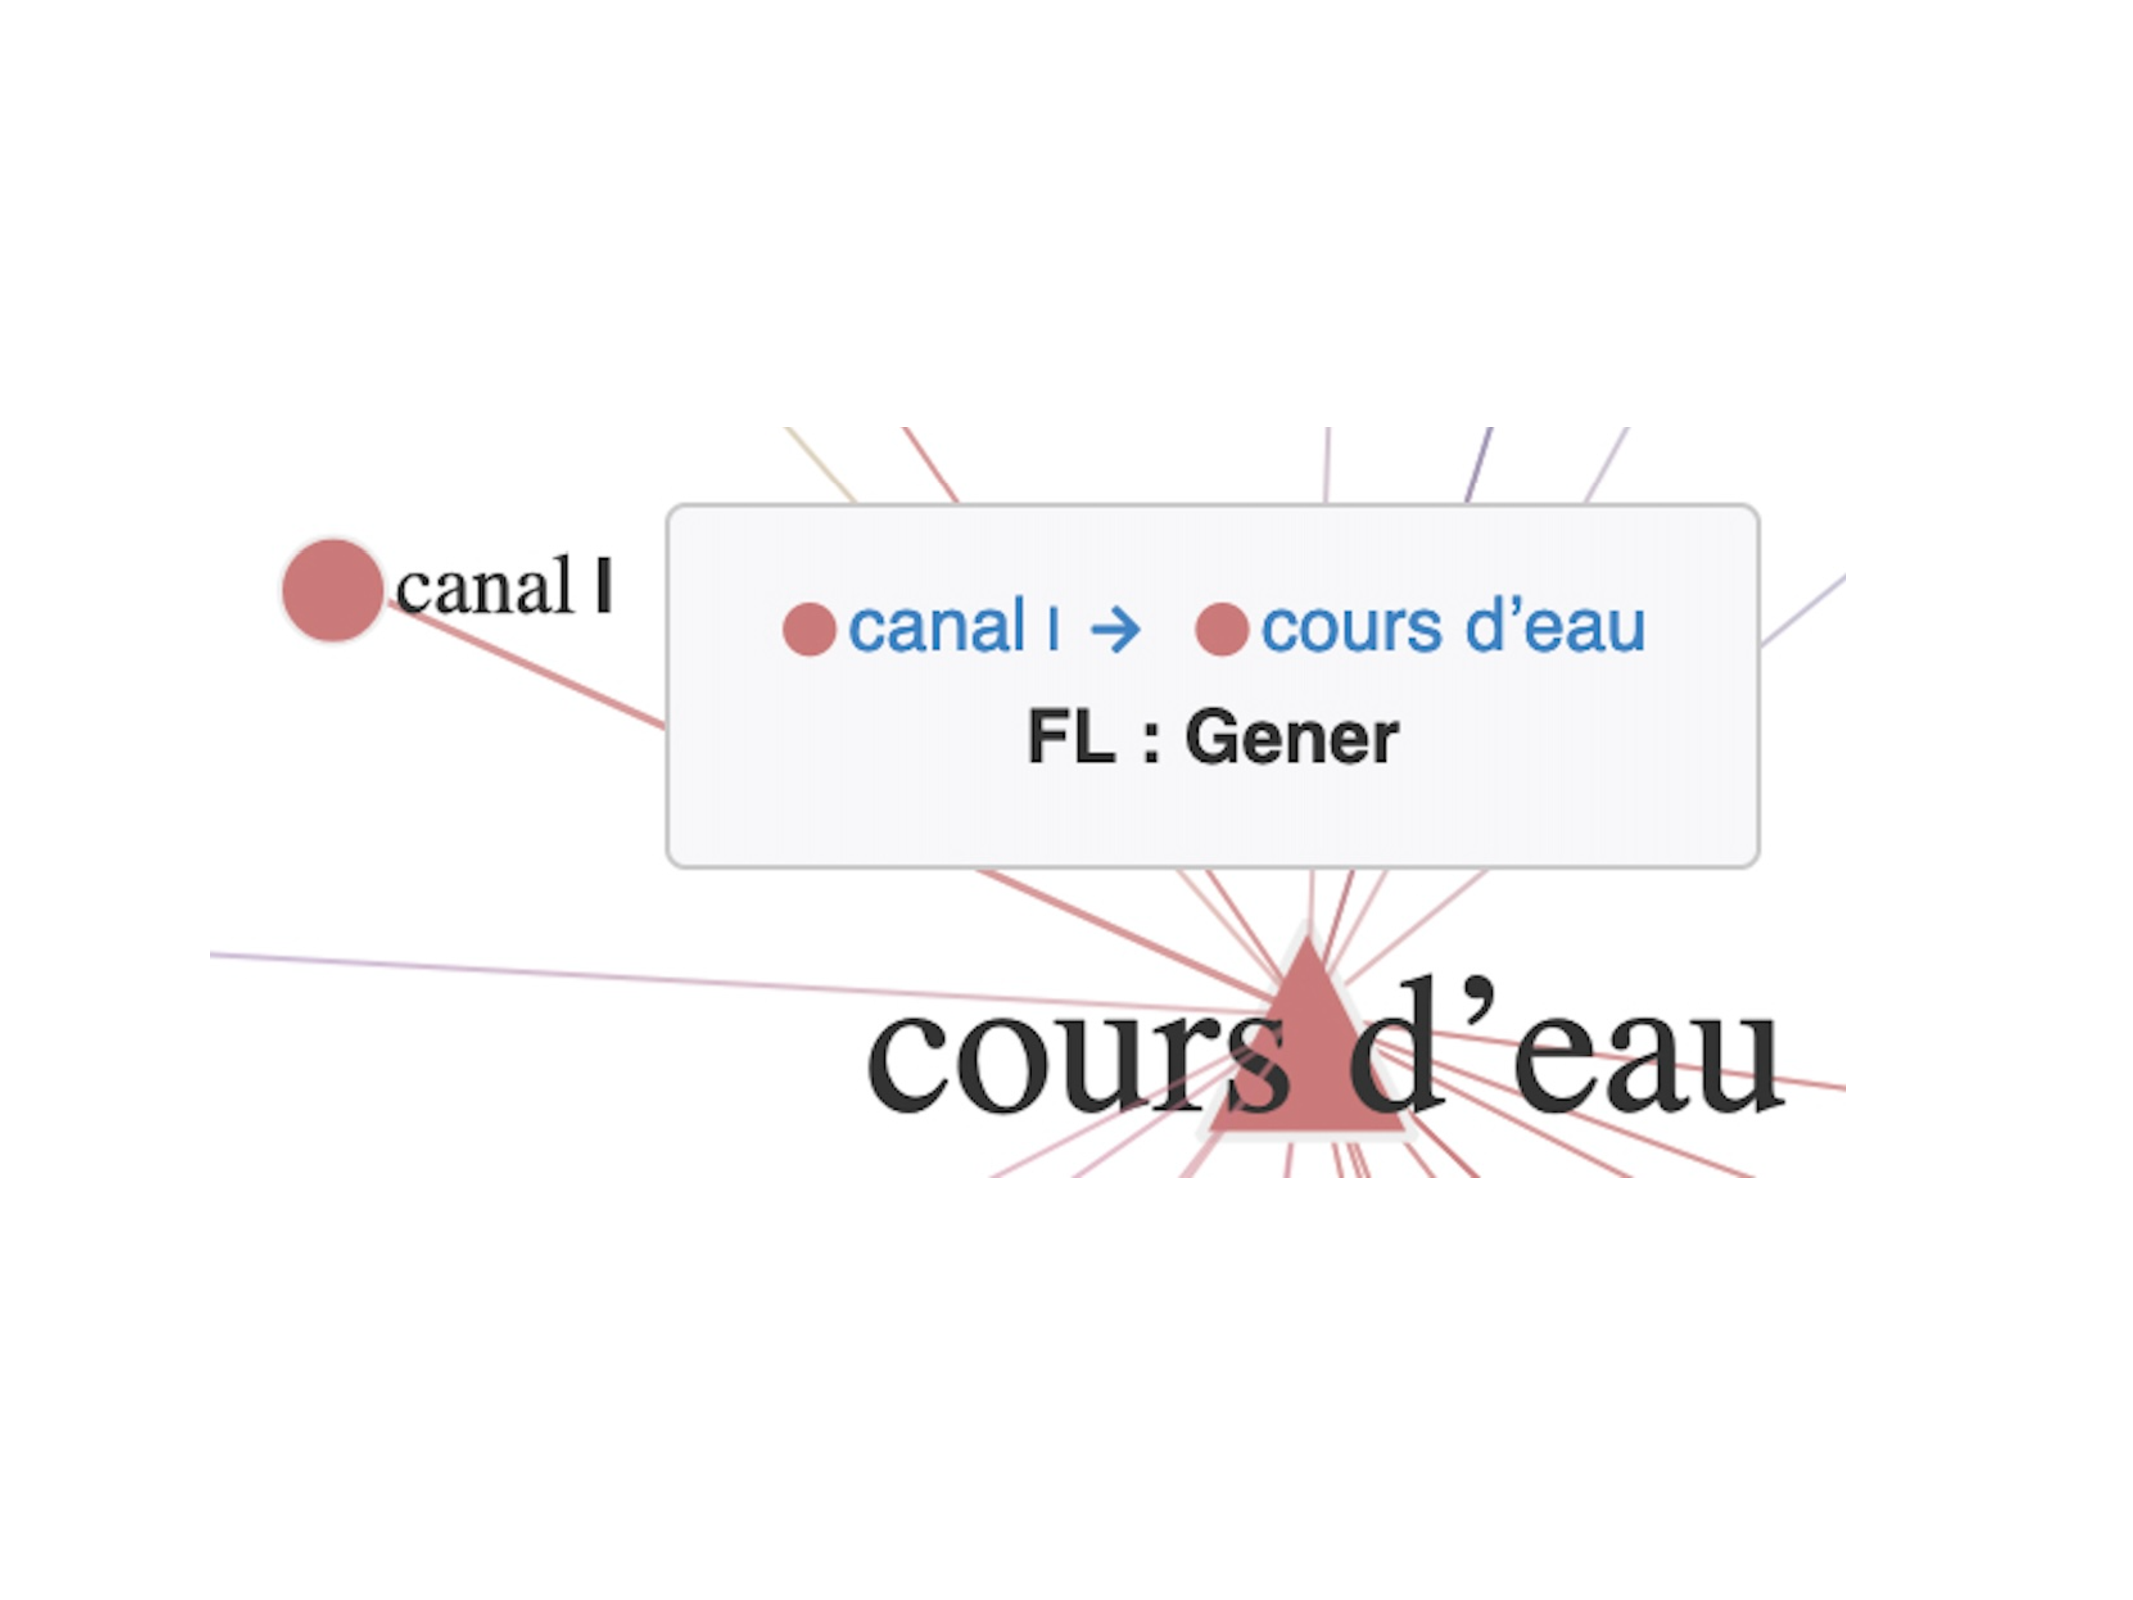
\epsfig{width=4cm,file=Fig/LexicalNetworks/canal-coursDEau.pdf}
\caption[\lfappl{Gener}{\textit{canal}\sensenum{I} {\footnotesize `\lfgp{water} canal'}} = \idiom{\textit{cours d'eau}} {\footnotesize `watercourse'} as represented in the fr-LN]{LF application \lfappl{Gener}{\textit{canal}\sensenum{I} {\footnotesize `\lfgp{water} canal'}} = \idiom{\textit{cours d'eau}} {\footnotesize `watercourse'} as represented in the fr-LN}\label{fig:canal-coursDEau}
\end{figure}

\phantomsection\label{rem:visualizationLS}\begin{soundbox}{Visualization of Lexical Systems}\index[notion]{visualization}
In the present chapter, we make use of a dedicated \notion{network browser}\index[notion]{network \lfgp{see also \textit{graph}}!\tld\ browser}, called \notion{Spiderlex}\index[notion]{Spiderlex|emph}, for the visualization of the content of Lexical Systems \parencite{OllingerEtAl2020,OllingerPolguere2020b-e}. Spiderlex exploits the mathematical properties of the small-world\index[notion]{small-world!\tld\ network}\index[notion]{network \lfgp{see also \textit{graph}}!small-world \tld}\index[notion]{lexical network} structure of Lexical Systems (\sectref{sec:formalPropertiesLS}, p.\thinspace\pageref{sec:formalPropertiesLS}) and plays an important role for the utilization of lexical data both by lexicographers and users of the fr-LN -- see \sectref{sec:lexicographyOfLNs}, p.\thinspace\pageref{sec:lexicographyOfLNs}. Note that the orientation of arcs\index[notion]{arc of a network\slashs{}graph!orientation of an \tld}\index[notion]{orientation of a network arc} and their labels\index[notion]{arc of a network\slashs{}graph!label of an \tld}\index[notion]{label of a network\slashs{}graph arc} are not displayed by default, as in \figref{fig:taxonomicNonTaxonomicLNs}, in order to keep the visualization legible; this information can be shown by pointing at individual arcs, as in \figref{fig:canal-coursDEau}.\footnotemark
\end{soundbox}\footnotetext{\label{fn:fr-LNDataEvolving}Data from the fr-LN used in this chapter and the screenshots from Spiderlex reflect the state of this constantly evolving model at time of writing.}

The notion of Lexical System, first introduced in \textcite{Polguere2009-e}, gradually took shape out of the practice of computational Explanatory Combinatorial Lexicography\index[notion]{lexicography!computational Explanatory Combinatorial \tld}\index[notion]{Explanatory Combinatorial!computational \tld\ Lexicography} \parencite{Steinlinetal2005,PolguereMelcuk2006}. It was based on the observation that the system of simple standard LFs\index[notion]{system of standard LFs}\index[notion]{lexical function!system of standard \tlds} -- in particular LFs identified in this book as being central\index[notion]{lexical function!central \tld\ (in the system of standard \tlds)} (\chapref{chap:NotionLF}, \sectref{sec:centralLFs}, p.\thinspace\pageref{sec:centralLFs}) -- was a good candidate as main contributor to the structuring of lexical knowledge\index[notion]{lexical knowledge}, better by all means than mainstream taxonomic\index[notion]{taxonomy} principles. This has lead to a second postulate, this time concerning the structure of Lexical Systems.

\phantomsection\label{txt:postulateStrucLS}\begin{soundbox}{Postulate 2: structure of Lexical Systems}
Lexical Systems, as network lexicon models, are primarily structured by standard LF relations.
\end{soundbox}

Postulate~2 implies that LF relations form the backbone of Lexical Systems. From a methodological viewpoint, the lexicographic\index[notion]{lexicography!\tld\ of lexical networks}\index[notion]{lexical network!lexicography of \tlds} process of building a Lexical System for a given natural language is driven by the weaving of standard LF relations within the lexical network \parencite{LuxPogodallaPolguere2011,Polguere2012e-e}.

Two properties of standard LFs can be put forward in support of the adoption of Postulate~2:

\begin{enumerate}

\item Standard LFs express constrained meanings (\chapref{chap:NotionLF}, \pageref{sec:LFDefinitionNotion}, p.\thinspace\pageref{txt:constrainedMeaning})\index[notion]{meaning!constrained \tld}, present in all natural languages; these meanings determine fundamental paradigmatic and syntagmatic relations between lexical units.

\item A standard LF is essentially related to the meaning of each individual lexical unit L it takes as argument, in the sense that it is anchored in L's definition\index[notion]{definition!lexicographic \tld} -- cf. the notion of LF target\index[notion]{lexical function!target of a \tld}\index[notion]{target of an LF} (\chapref{chap:NotionLF}, \sectref{sec:classeFLSyntagmatiques}, p.\thinspace\pageref{txt:targetOfSyntLF}). Conversely, a standard LF can serve as a revealer of the presence of a particular semantic chunk in L's meaning \parencite{IordanskajaPolguere2005}.

\end{enumerate}

\paragraph*{Relational profile of a node\slashs{}lexical unit.}\label{par:relationalProfile}

Because of the above properties, it is justified to consider that each node\index[notion]{node of a network\slashs{}graph}\index[notion]{network \lfgp{see also \textit{graph}}!node of a \tld} \textit{n} of a Lexical System -- and the corresponding lexical unit L -- has a \notion{relational profile}\index[notion]{relational profile|emph}\index[notion]{profile, relational|emph} consisting of two sets: the set of \textit{n}'s outgoing arcs and the set of its incoming arcs.

\begin{itemize}

\item The set of \textit{n}'s outgoing arcs\index[notion]{arc of a network\slashs{}graph!outgoing \tld}\index[notion]{network \lfgp{see also \textit{graph}}!arc of a \tld} -- i.e., L's \notion{outgoing profile}\index[notion]{relational profile!outgoing \tld}\index[notion]{profile, relational!outgoing \tld} -- is the main constituent of L's relational profile as it is a reflection of the essential semantic and combinatorial properties of L. It corresponds to the information listed in the cooccurrence zone\index[notion]{lexical entry!cooccurence zone of a \tld}\index[notion]{zone of a lexical entry!cooccurrence \tld} in an Explanatory Combinatorial Dictionary\index[notion]{Explanatory Combinatorial!\tld\ Dictionary}\index[notion]{dictionary!Explanatory Combinatorial \tld} -- see Appendix, p.\thinspace\pageref{sec:AppendixLFZone}.

\item The set of \textit{n}'s incoming arcs\index[notion]{arc of a network\slashs{}graph!incoming \tld} -- i.e., L's \notion{incoming profile}\index[notion]{relational profile!incoming \tld}\index[notion]{profile, relational!incoming \tld} -- is a relational information that is \emph{not} present in the cooccurrence zone of L's lexical entry in an Explanatory Combinatorial Dictionary\index[notion]{Explanatory Combinatorial!\tld\ Dictionary}\index[notion]{dictionary!Explanatory Combinatorial \tld} and, more importantly, that is simply not encoded in this type of model. In a Lexical System, by contrast, incoming profiles are embedded in the model's network structure and can be accessed directly.

\end{itemize}

This is illustrated in	\figref{fig:outgoingIncomingProfile}, with an adaptation of the Spiderlex\index[notion]{Spiderlex} visualization\index[notion]{visualization} of both the current outgoing and incoming profiles of {\smaller French}~\textsc{sentiment}\sensenum{1a} `feeling' in the fr-LN. The complementarity of the two profiles is well illustrated by the contrast between the unique outgoing \lf{Gener}\index[lf]{Gener@\lf{Gener}} relation (towards {\smaller French}~\textit{état psychique} `psychological state') and the large set of incoming \lf{Gener} relations, which characterizes {\smaller French}~\textsc{sentiment}\sensenum{1a} as being a generic term\index[notion]{generic term} (i.e., classifying lexical unit) in the French lexicon\index[notion]{noun!\tld\ of feeling}.

\begin{figure}

\scriptsize
\setlength{\tabcolsep}{1pt}
\setlength\extrarowheight{1.2pt}
\APolbox{5.3cm}{%
\begin{tabular}{ l c >{\raggedright\arraybackslash}p{3.4cm} }
\multicolumn{3}{ c }{{\small \textsf{Outgoing LF relations}}} \\[+4pt]
\lf{Syn$_\supset$}
& :
& \textit{émotion}\sensenum{2} \\
\lf{Syn$_\cap$}
& :
& \textit{sensation}\sensenum{1}\textbf{,}  \uslabel{spec} \textit{affect}\sensenum{a}\textbf{;} \uslabel{spec} \textit{état émotionnel} \\
\lf{Gener}
& :
& \uslabel{(spec)} \textit{état psychique} \\
\lf{S$_\text{loc}^\text{prototyp}$}
& :
& \textit{cœur}\sensenum{III.1}\textbf{;} \textit{âme}\sensenum{I}\textbf{,} \textit{esprit}\sensenum{I.1} \\
\lf{Magn}
& :
& \textit{vif}\sensenum{II.2}\textbf{,} \textit{profond}\tsub{(Adj)}\sensenum{II}\textbf{,} \textit{fort}\tsub{(Adj)}\sensenum{III.2} \\
\lf{Oper\tsub{1}}
& :
& \textit{éprouver}\sensenum{a} \lfgp{\textsc{art} \tld}\textbf{,}  \textit{ressentir} \lfgp{\textsc{art}~\tld}\textbf{;} \textit{nourrir}\sensenum{II.1} \lfgp{\textsc{art} \tld}\textbf{,} \textit{avoir}\sensenum{VII.2} \lfgp{\textsc{art} \tld} \\
\lf{Func\tsub{1}}
& :
& \textit{habiter}\sensenum{II} \lfgp{N\tsub{X}} \textbf{<} \textit{étreindre}\sensenum{II} \lfgp{N\tsub{X}} \textbf{<} \textit{submerger}\sensenum{II} \lfgp{N\tsub{X}} \\
\lf{IncepFunc\tsub{1}}
& :
& \textit{naître}\sensenum{II} \lfgp{\textit{en} N\tsub{X}}\textbf{,} \textit{envahir}\sensenum{III} \lfgp{N\tsub{X}}\textbf{,} \textit{saisir}\sensenum{III} \lfgp{N\tsub{X}}\textbf{,}  \textit{prendre}\sensenum{VIII} \lfgp{N\tsub{X}} \textbf{<} \textit{s'emparer}\sensenum{II.2} \lfgp{\textit{de} N\tsub{X}} \\
\lf{Caus\tsub{1}Func\tsub{2'}}
& :
& \textit{transférer}\sensenum{III} \lfgp{\textsc{art} \tld\ \textit{sur} N\tsub{Y'}} \\
\lf{Fact\tsub{1}}
& :
& \textit{guider}\sensenum{II} \lfgp{N\tsub{X}}\textbf{,} \textit{animer}\sensenum{III} \lfgp{N\tsub{X}} \\
\lf{IncepManif}
& :
& \textit{se peindre} \lfgp{\textit{sur} N} \\
\multicolumn{3}{c}{} \\[59pt]
\end{tabular}
}
\hphantom{.}
\APolbox{6.6cm}{%
\begin{tabular}{ l c >{\raggedright\arraybackslash}p{5cm} }

\multicolumn{3}{ c }{{\small \textsf{Incoming LF relations}}} \\[+4pt]

\lf{Syn$_\subset$}
& \textsf{\textbf{for}}
& \textit{émotion}\sensenum{2} \\

\lf{Syn$_\cap$}
& \textsf{\textbf{for}}
& \textit{affect}\sensenum{a}\thinspace-- \textit{état émotionnel}\thinspace-- \textit{sensation}\sensenum{1} \\

\lf{Gener}
& \textsf{\textbf{for}}
& \textit{admiration}\thinspace-- \textit{allégresse}\thinspace-- \textit{amour}\sensenum{I.1a}\thinspace-- \textit{amour}\sensenum{I.1b}\thinspace-- \textit{animosité}\sensenum{1}\thinspace-- \textit{appitoiement}\sensenum{a}\thinspace-- \textit{appitoiement}\sensenum{b}\thinspace-- \textit{aversion}\thinspace-- \textit{bonheur}\sensenum{1}\thinspace-- \textit{cafard}\sensenum{II}\thinspace-- \wf{chagrin}{(N)}{1}{1}\thinspace-- \textit{colère}\sensenum{1}\thinspace-- \textit{compassion}-- \textit{contentement}\thinspace-- \textit{curiosité}\sensenum{I.2}\thinspace-- \textit{déception}\thinspace-- \textit{dégoût}\sensenum{II}\thinspace-- \textit{déprime}\thinspace-- \textit{désespoir}\sensenum{1}\thinspace-- \textit{désir}\sensenum{1}\thinspace-- \textit{désir}\sensenum{2}\thinspace-- \textit{dévastation}\sensenum{II.2}\thinspace-- \textit{doute}\thinspace-- \textit{effroi}\thinspace-- \textit{émoi}\thinspace-- \textit{émotion}\sensenum{1}\thinspace-- \textit{empathie}\thinspace-- \textit{étonnement}\thinspace-- \textit{fierté}\sensenum{I.1}\thinspace-- \textit{frayeur}\thinspace-- \idiom{\textit{froid dans le dos}}\thinspace-- \textit{frousse}\thinspace-- \textit{frustration}\thinspace-- \textit{fureur}\sensenum{I}\thinspace-- \textit{gratitude}\thinspace-- \textit{haine}\sensenum{1}\thinspace-- \textit{haine}\sensenum{2}\thinspace-- \textit{honte}\sensenum{I.1}\thinspace-- \textit{horreur}\sensenum{I}\thinspace-- \textit{horreur}\sensenum{II}\thinspace-- \textit{humiliation}\sensenum{2}\thinspace-- \textit{jalousie}\sensenum{I}\thinspace-- \idiom{\textit{mal au cœur}}\sensenum{II}\thinspace-- \idiom{\textit{mal du pays}}\thinspace-- \textit{malaise}\sensenum{3}\thinspace-- \textit{mécontentement}\thinspace-- \textit{mélancolie}\sensenum{II.1}\thinspace-- \textit{mépris}\thinspace-- \textit{nausée}\sensenum{II}\thinspace-- \textit{nostalgie}\sensenum{I}\thinspace-- \textit{orgueil}\sensenum{2a}\thinspace-- \textit{peur}\sensenum{1}\thinspace-- \textit{plaisir}\sensenum{I.1}\thinspace-- \textit{rage}\sensenum{II}\thinspace-- \textit{ravissement}\thinspace-- \textit{reconnaissance}\sensenum{II}\thinspace-- \textit{répugnance}\sensenum{1}\thinspace-- \textit{répulsion}\sensenum{I}\thinspace-- \textit{ressentiment}\thinspace-- \textit{satisfaction}\sensenum{II}\thinspace-- \textit{sentiment}\sensenum{1b}\thinspace-- \textit{souci}\sensenum{1}\thinspace-- \textit{spleen}\thinspace-- \textit{tristesse}\sensenum{I}\thinspace-- \textit{trouille}  \\


\lf{S$_\text{2}$}
& \textsf{\textbf{for}}
& \textit{éprouver}\sensenum{a} \\

\lf{S$_\text{2}^\text{prototyp}$}
& \textsf{\textbf{for}}
& \textit{émoji} \\

\lf{S$_\text{3}^\text{prototyp}$}
& \textsf{\textbf{for}}
& \textit{chantage}\sensenum{II} \\

\end{tabular}
}
\caption[Outgoing vs. incoming profiles of {\smaller French}~\textsc{sentiment}\sensenum{1a} `feeling' in the fr-LN]{Outgoing vs. incoming profiles of {\smaller French}~\textsc{sentiment}\sensenum{1a} `feeling' in the fr-LN}\label{fig:outgoingIncomingProfile}
\end{figure}

\figref{fig:outgoingIncomingProfile} shows that Lexical Systems' data need not be visualized graphically. Textual, dictionary-like visualizations similar to lexical entries of a traditional dictionary can also be generated from the same data. For this reason, the construction of Lexical Systems is presented in \textcite{Polguere2012d-e} as being a \notion{lexicography of virtual dictionaries}.\index[notion]{visualization!textual \tld}\index[notion]{lexical entry!automatically generated \tld}\index[notion]{dictionary!virtual \tld}\index[notion]{lexicography!\tld\ of virtual dictionaries}

Incoming profiles can play an important role in applications of lexical network models, for instance, in language teaching\index[notion]{teaching\slashs{}learning, language}\index[notion]{language teaching\slashs{}learning}. Thus, the meaning of the generic term\index[notion]{generic term} \textsc{precipitation}\sensenum{1} `type of weather condition'\footnote{The lexicographic number of \textsc{precipitation}\sensenum{1} comes from the LDOCE.}\index[notion]{dictionary!Longman Dictionary of Contemporary English@\textit{Longman Dictionary of Contemporary English} [LDOCE]}\index[notion]{Longman Dictionary of Contemporary English@\textit{Longman Dictionary of Contemporary English} [LDOCE]}\index[notion]{lexicographic number} is better taught to language learners by relying on this term's incoming profile, i.e., by listing some of the most typical lexical units for which \textsc{precipitation}\sensenum{1} is a \lf{Gener} -- \textsc{rain}\tsub{(N)}, \textsc{snow}\tsub{(N)}, \textsc{hail}\tsub{(N)}, etc. -- as most dictionaries do.\footnote{See, for instance, the largely enumerative definition of LDOCE: `any form of water, such as rain, snow, sleet, or hail, that falls to the Earth's surface'. On defining so-called \textit{functional collective superordinates} within the Natural Semantic Metalanguage approach, see \textcite{Goddard2017}.}\index[notion]{dictionary!Longman Dictionary of Contemporary English@\textit{Longman Dictionary of Contemporary English} [LDOCE]}\index[notion]{Longman Dictionary of Contemporary English@\textit{Longman Dictionary of Contemporary English} [LDOCE]}\index[notion]{definition!lexicographic \tld}\index[notion]{Natural Semantic Metalanguage} This is probably a better pedagogical strategy than trying to first provide learners with a lexicographic definition\index[notion]{definition!lexicographic \tld} that can only be non-specific and will be felt as more confusing than explanatory.

This observation does not necessarily apply to any generic terms, in particular to generic terms with more specific meanings, for which a lexicographic definition can be a good starting point in vocabulary teaching -- e.g., generic terms such as \textsc{bird}, \textsc{tree}\tsub{(N)}, etc. Collocative lexical units\index[notion]{lexical unit!collocative \tld} -- lexical units that are essentially selected by the Speaker\index[notion]{Speaker, the} as collocates\index[notion]{collocation!collocate of a \tld} in collocations -- are another illustration of the usefulness of incoming profiles. Thus, the intensifier \lu{heavy}{(Adj)}{}{2}\phantomsection\label{txt:HEAVY-Adj-2} \senseex{heavy rain}\footnote{The lexicographic number of \lu{heavy}{(Adj)}{}{2} comes from the LDOCE.}\index[notion]{dictionary!Longman Dictionary of Contemporary English@\textit{Longman Dictionary of Contemporary English} [LDOCE]}\index[notion]{Longman Dictionary of Contemporary English@\textit{Longman Dictionary of Contemporary English} [LDOCE]}\index[notion]{lexicographic number} controls very few outgoing LF relations and its relational profile resides essentially in all its incoming \lf{Magn}\index[lf]{Magn@\lf{Magn}} relations -- the set of all lexical units for which it is a \lf{Magn} (\textsc{accent}\tsub{(N)}, \textsc{accusation}, \textsc{applause}, \textsc{battle}\tsub{(N)}, \textsc{blow}\tsub{(N)}, \textsc{emphasis}, \textsc{fog}\tsub{(N)}, etc.). The meaning of \lu{heavy}{(Adj)}{}{2} is simply that of \lf{Magn} -- the same constrained meaning\index[notion]{meaning!constrained \tld} as for dozens of adjectival intensifiers in English; consequently, its incoming profile is as important as its definition in the acquisition\index[notion]{acquisition!lexical \tld} of this lexical unit by language learners.\footnote{It is interesting to contrast two types of dictionaries of collocations in the light of the notion of relational profile: (i) those whose entries are collocation bases and that provide the list of collocates they select -- see \textcite{BensonEtAl2010} for English and \textcite{Bosque2006} for Spanish; (ii)~those whose entries are collocates and that provide the list of corresponding bases in collocations -- see \textcite{Bosque2010} for Spanish. The former describe the outgoing relational profile of bases, while the latter describe the incoming relational profile of collocates.}\index[notion]{dictionary!\tld\ of collocations}\index[notion]{collocation!dictionary of \tlds}

\paragraph*{Semantic weight of LF relations.}\label{par:semanticWeightLFRelation}

All LF relations found in the relational profile of a given lexical unit L do not carry the same \notion{semantic weight}.\index[notion]{weight, semantic|emph}\index[notion]{semantic!\tld\ weight|emph}\footnote{The notion of semantic weight is further developed in \sectref{sec:formalPropertiesLS}, p.\thinspace\pageref{sec:formalPropertiesLS}.} Indeed, LFs are very diverse with respect to the semantic proximity they \emph{inherently} imply -- or not -- between their argument and their value. For instance, \lfappl{Syn}{L\tsub}\index[lf]{Syn@\lf{Syn}} = L′, \lfappl{V\tsub{0}}{L}\index[lf]{V0@\lf{V\tsub{0}}} = L′, \lfappl{A\tsub{1}}{L}\index[lf]{Ai@\lf{A\tsub{i}}!\lf{A\tsub{1}}} = L′, etc., obviously imply a strong \notion{meaning relation}\index[notion]{meaning!\tld\ relation|emph}\index[notion]{relation!meaning \tld|emph} between L and L′, as L′ is a semantic derivative\index[notion]{derivative!semantic \tld}\index[notion]{semantic!\tld\ derivative} of L. By contrast, \lfappl{Magn}{L}\index[lf]{Magn@\lf{Magn}} = L′, \lfappl{Loc\tsub{in}}{L}\index[lf]{Locin@\lf{Loc\tsub{in}}} = L′, \lfappl{Oper\tsub{1}}{L}\index[lf]{Operi@\lf{Oper\tsub{i}}!\lf{Oper\tsub{1}}}~= L′, etc., do not inherently imply any meaning relation between L and L′; such relation may exist ``incidentally,'' for a given case of \lfappl{f}{L} = L′, but not by virtue of the meaning \sigmaF\ of \lf{f} -- e.g., \lfappl{Magn}{\textit{appetite}} = \textit{ravenous} -- where \textit{appetite} means approximately `desire to eat' and \textit{ravenous}, when used freely (i.e., not as as an intensifier), means `who has a strong desire\slashs{}need to eat'.

In a Lexical System, each arc of the network that corresponds to an LF relation carries a semantic weight which is determined by the meaning \sigmaF\ of the corresponding LF \lf{f}. Prototypically, arcs corresponding to paradigmatic LFs (i.e., leading to semantic derivatives)\index[notion]{lexical function!paradigmatic vs. syntagmatic \tlds} tend to carry a stronger semantic weight than those corresponding to syntagmatic LFs. We will see shortly (\sectref{sec:non-LFRelationsInLSs}) that the notion of semantic weight also applies to non-LF relations.

Before proceeding with the examination of lexical relations in Lexical Systems that are not based on LFs, it is important to note that a given node \textit{n} of a Lexical System is a complex informational entity that encapsulates all the properties of the corresponding lexical unit L not accounted for by LF relations: grammatical characteristics, lexicographic definition\index[notion]{definition!lexicographic \tld}, etc. That is, the lexical properties specified in \textit{n} together with \textit{n}'s relational profile are informationally equivalent to a lexical entry\index[notion]{lexical entry} for L. Of course, in the context of the lexicography of lexical networks\index[notion]{lexicography!\tld\ of lexical networks}\index[notion]{lexical network!lexicography of \tlds} \parencite{Polguere2014c-e}, special lexicographic tools are required to construct individual nodes with their individual properties and to weave the relations between nodes (see \sectref{sec:lexicographyOfLNs}, p.\thinspace\pageref{sec:lexicographyOfLNs}).

\subsubsection{Non-LF relations between lexical units}\label{sec:non-LFRelationsInLSs}

Three non-LF relations\index[notion]{lexical relation!non-LF \tld} play an important role in Lexical Systems:

\begin{itemize}

\item copolysemy relation, holding between two lexical units of a polysemous vocable (\sectref{sec:copolysemyRelation});

\item idiom-component relation, holding between an idiom and a lexeme that participates in its surface-syntactic structure (\sectref{sec:idiomComponentRelation});

\item meaning-inclusion relation, holding between a lexical unit and another lexical unit that is an element of its lexicographic definition (\sectref{sec:meaningInclusionRelation}).

\end{itemize}

To make the presentation of these relations more straightforward and concrete, we base the following explanation mostly on data borrowed from the fr-LN.\index[notion]{French Lexical Network [fr-LN]}\index[notion]{lexical database!French Lexical Network [fr-LN]}\index[notion]{lexical network!French \tld\ [fr-LN]}

The order of presentation of the three non-LF relations is determined by the expertise that has been gained from lexicographic work on the fr-LN: from the most extensively described relations to those whose encoding is still at an experimental stage.

Finally, note that the relational profile\index[notion]{relational profile}\index[notion]{profile, relational} of a node\slashs{}lexical unit, while primarily based on LF relations, also includes the three relations that are presented below.

\subsubsubsection{Copolysemy relation}\label{sec:copolysemyRelation}

The fr-LN -- as should be the case of any full-fledged Lexical System -- contains the explicit modeling of the \notion{polysemy structure}\index[notion]{polysemy!\tld\ structure of a vocable|emph}\index[notion]{vocable!polysemy structure of a \tld|emph} of vocables through the encoding of so-called \notion{copolysemy relations}\index[notion]{polysemy!co\tld|emph}\index[notion]{copolysemy|emph}\index[notion]{lexical relation!copolosemy \tld|emph}\index[notion]{relation!copolysemy \tld|emph} between lexical units of a vocable. A copolysemy relation -- that is, the corresponding arc of the lexical network -- is oriented from the lexical unit that is the source of the ``copolysemy derivation'' toward the ``derived'' lexical unit. In other words, L\thinspace\lexRel{copolysemy}\thinspace{}L′ reads as `lexical unit L has lexical unit L′ as its copolysemy extension, metonymy, metaphor, ...'; this relation participates in the polysemy structure of a given vocable.

Some copolysemy relations have a strong semantic weight\index[notion]{semantic!\tld\ weight}\index[notion]{weight, semantic}\index[notion]{arc of a network\slashs{}graph!semantic weight of an \tld} in the network: they imply that the two lexical units they connect belong to identical semantic fields\index[notion]{semantic!\tld\ field}. This is the case of the metonymy\index[notion]{metonymy}\index[notion]{copolysemy!\tld\ relation of metonymy} relation that links {\smaller French}~\textsc{cigarette}\sensenum{I} `cigarette'\phantomsection\label{txt:CIGARETTE} to {\smaller French}~\textsc{cigarette}\sensenum{II} `habit of smoking \textit{cigarettes}\sensenum{I}'\footnote{Cf. \textit{Julie veut arrêter la cigarette} `Julie wants to stop smoking cigarettes'. There is no corresponding lexical unit in English. The polysemy of {\smaller French}~\textsc{cigarette} is chosen as illustration for two reasons: (i)~it is not identical to that of {\smaller English}~\textsc{cigarette}, which highlights the relevance of explicitly encoding polysemy structures, in particular, for the study of regular polysemy \parencite{Apresjan1974,PetersWPetersI2000,Polguere2022a}; (ii)~though not too rich, it displays both metonymy and metaphor copolysemy relations, which we use later to illustrate the modeling of lexical proximity in lexical networks (\sectref{sec:lexicalProximityTopologicalProximity}, ``\nameref*{par:lexicalSpaces},'' p.\thinspace\pageref{par:lexicalSpaces}).}\index[notion]{polysemy!regular \tld}\index[notion]{regularity!regular polysemy} -- see \figref{fig:polysemyCIGARETTE}. Other copolysemy relations have weak (or, even, null) semantic weight -- for instance, the metaphor\index[notion]{metaphor}\index[notion]{copolysemy!\tld\ relation of metaphor} relation (based on shape) that links {\smaller French}~\textsc{cigarette}\sensenum{I} to the appositive noun {\smaller French}~\textsc{cigarette}\sensenum{III} `\lfgp{piece of clothing X} long and tight against the body, \idiom{as if} it had the shape of a \textit{cigarette}\sensenum{I}' (\textit{une robe cigarette} `a cigarette dress'). Such relations connect lexical units that are not expected to belong to the same semantic fields.

\begin{figure}

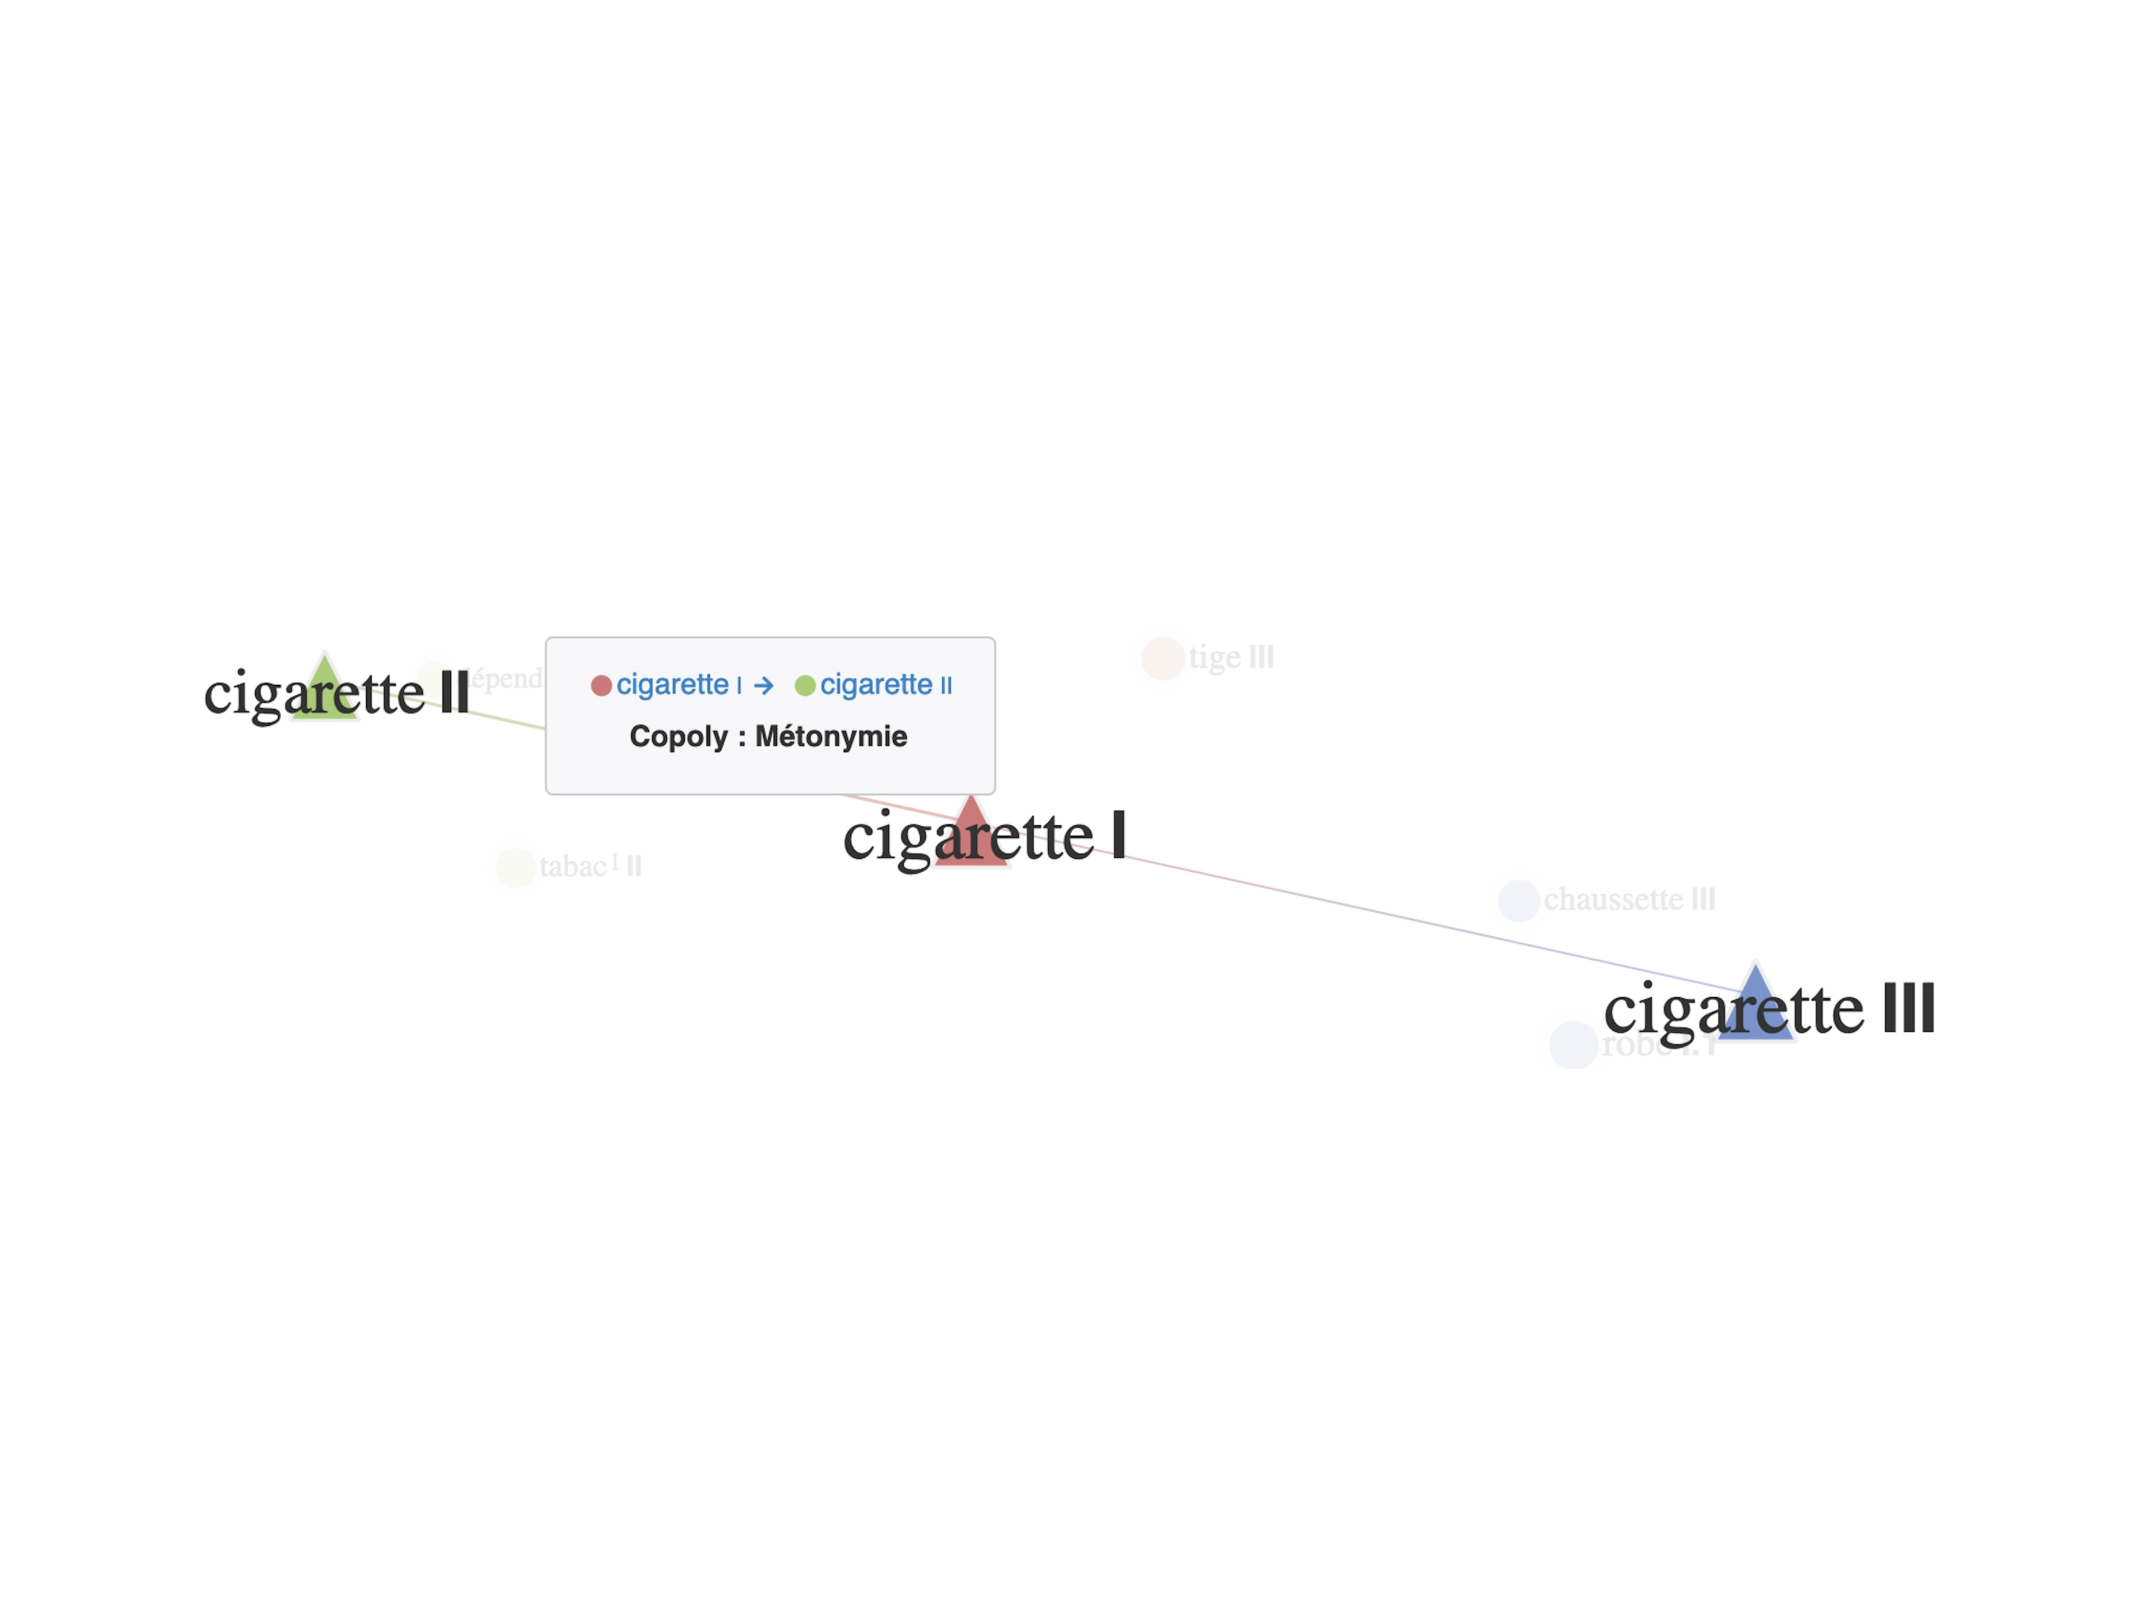
\epsfig{width=8cm,file=Fig/LexicalNetworks/polysemy-Fr-CIGARETTE.pdf}
\caption{Polysemy of {\smaller French}~\textsc{cigarette} as represented in the fr-LN}\label{fig:polysemyCIGARETTE}
\end{figure}

A polysemous vocable is formally encoded in a Lexical System as a subnetwork consisting of nodes connected by copolysemy arcs, as shown in \figref{fig:polysemyCIGARETTE} where two copolysemy arcs originate from the node \textsc{cigarette}\sensenum{I}. The \notion{basic lexical unit}\index[notion]{basic lexical unit of a vocable}\index[notion]{vocable!basic lexical unit of a \tld} of a given vocable -- i.e., the lexical unit that controls the polysemy structure of this vocable -- corresponds to the unique node in the subnetwork that does not have an incoming copolysemy arc in its relational profile\index[notion]{relational profile}\index[notion]{profile, relational}.

\subsubsubsection{Idiom-component relation}\label{sec:idiomComponentRelation}

In a Lexical System, an \notion{idiom-component relation}\index[notion]{lexical relation!idiom-component \tld|emph}\index[notion]{relation!idiom-component \tld|emph}\index[notion]{idiom!\tld-component relation|emph} encodes the presence of a lexeme in the surface-syntactic structure\index[notion]{idiom!surface-syntactic structure [SSyntS] of an \tld}\index[notion]{structure!surface-syntactic \tld\ [SSyntS]}\index[notion]{surface-syntactic!\tld\ structure [SSyntS]} [SSyntS] of an idiom \parencite{Pause2017b,Pause2017a}. This is illustrated in \figref{fig:idiomComponentRelBRAS_CASSE}, with the SSyntS of the French nominal idiom \idiom{\textsc{bras cassé}} lit.~`arm broken' -- which means approximately `bungler' -- and the corresponding idiom-component relations encoded in the fr-LN.

\begin{figure}

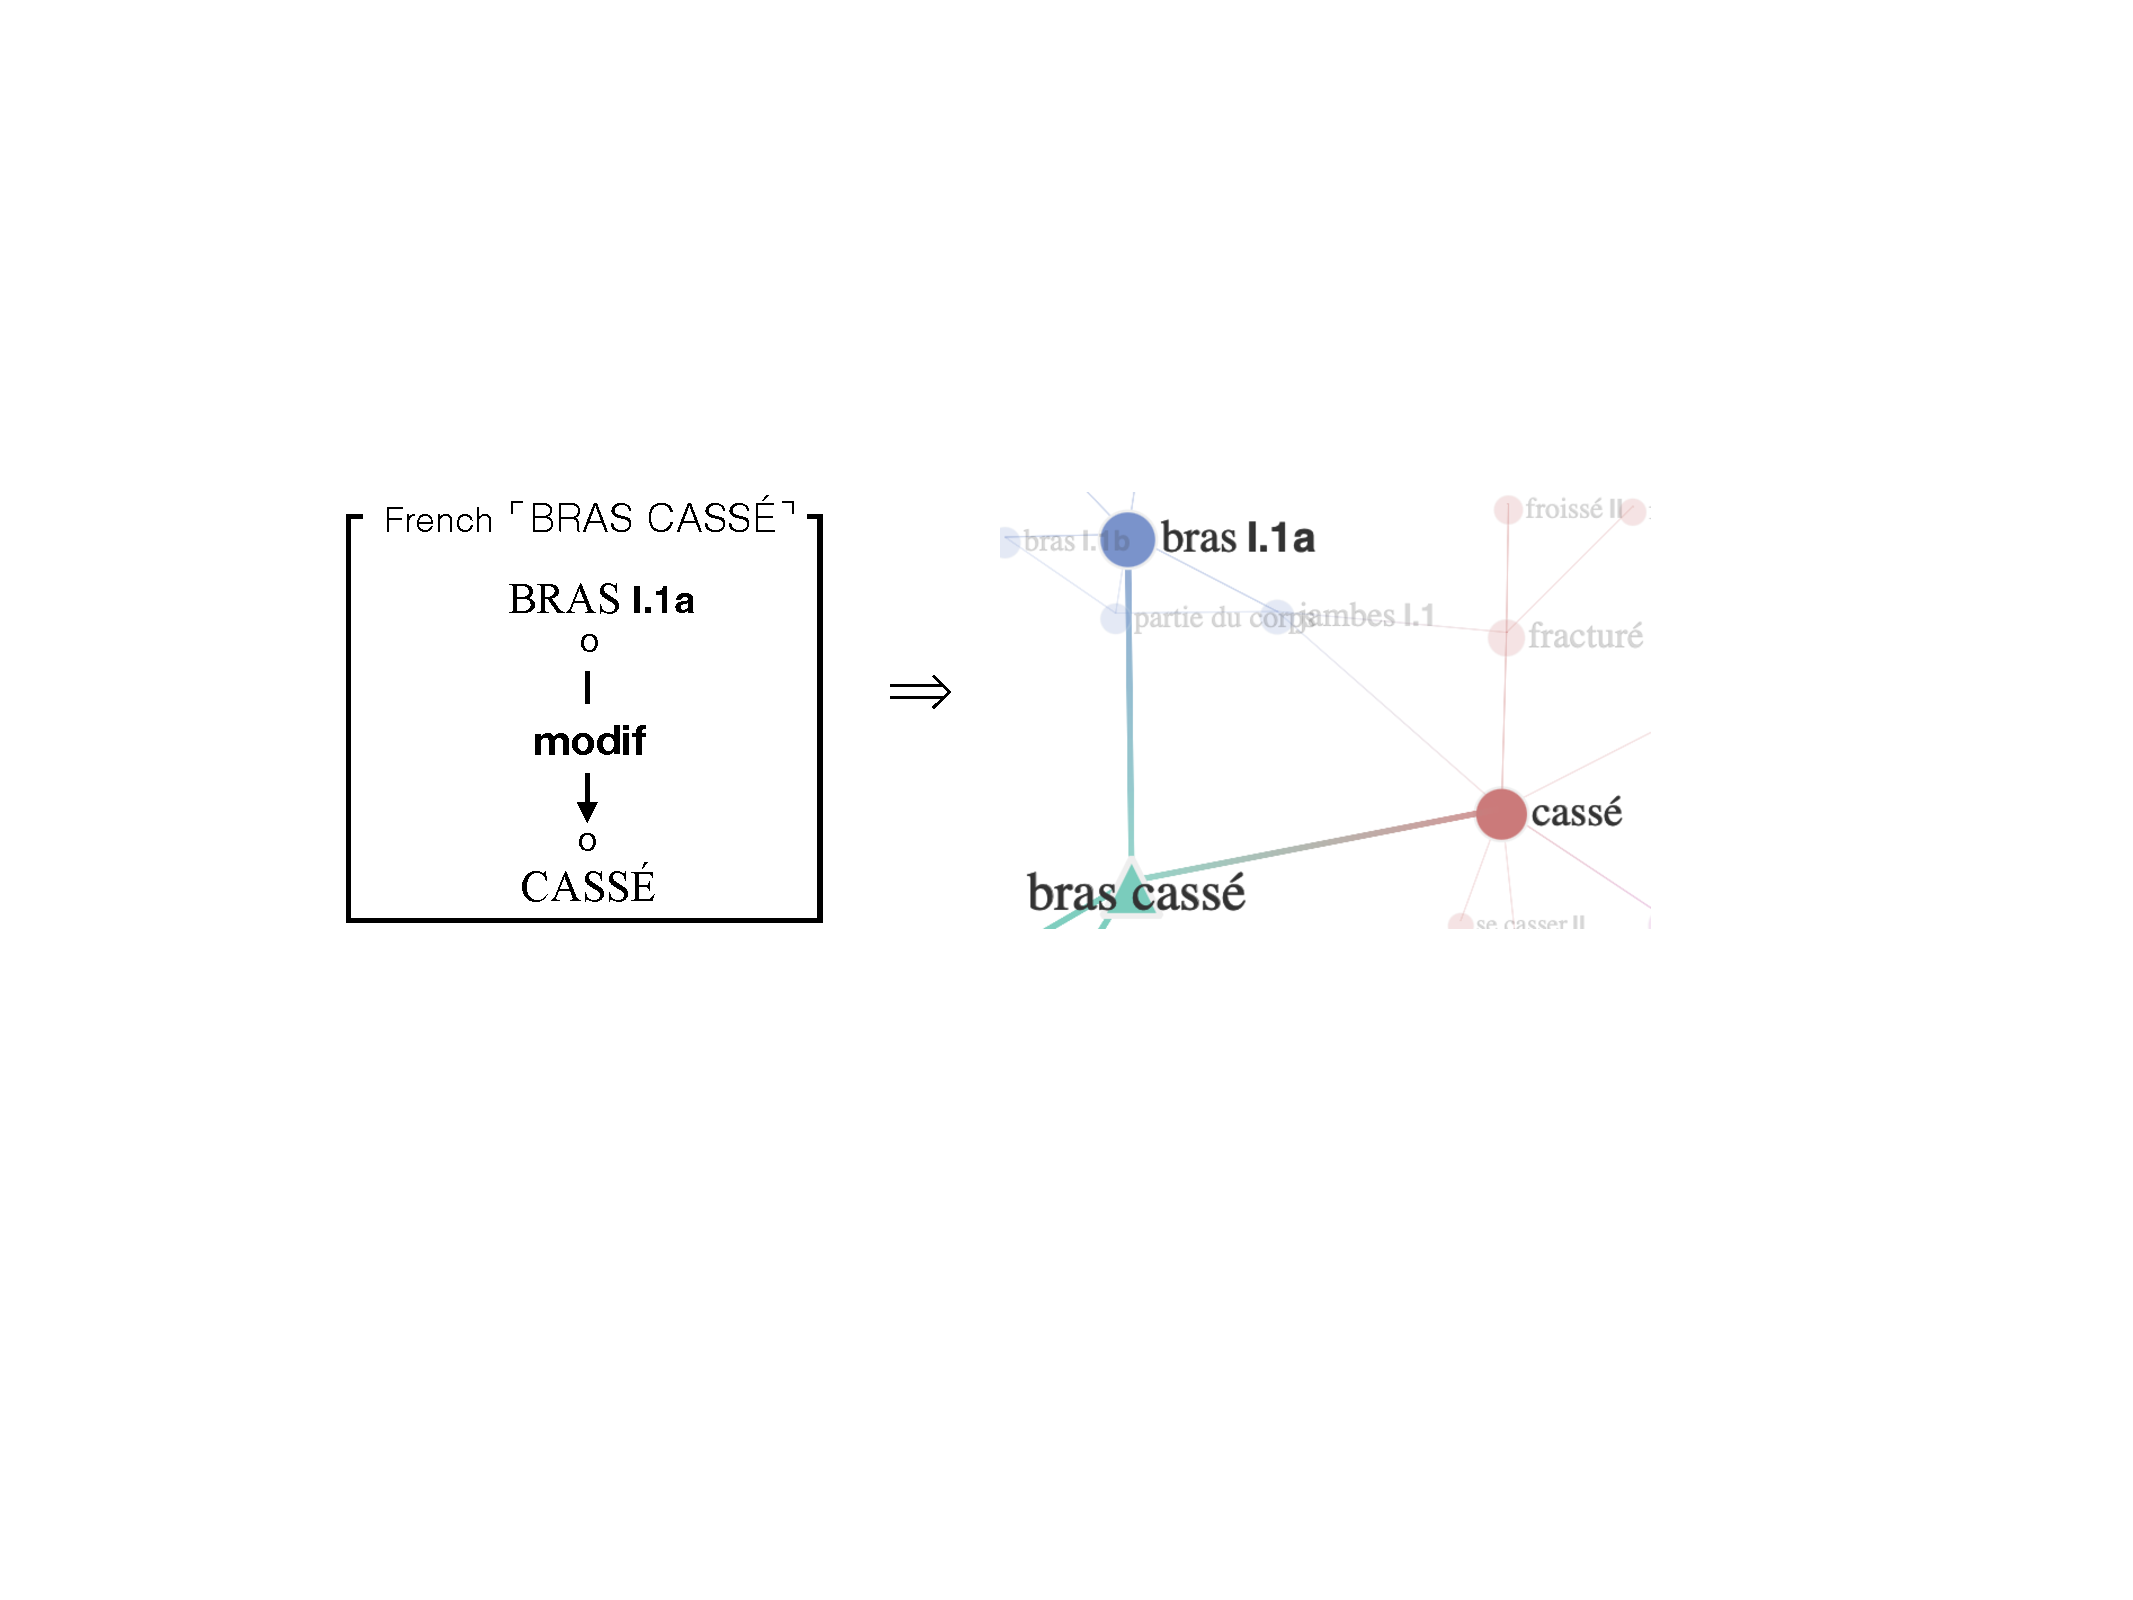
\includegraphics[width=.8\linewidth]{Fig/LexicalNetworks/idiomComponentRelBRAS_CASSE.pdf}
\caption[SSyntS of {\smaller French}~\idiom{\textsc{bras cassé}}~`bungler' and corresponding idiom-component relations in the fr-LN]{SSyntS of {\smaller French}~\idiom{\textsc{bras cassé}} `bungler' together with the two corresponding idiom-component relations encoded in the \mbox{fr-LN}\footnotemark}\label{fig:idiomComponentRelBRAS_CASSE}
\end{figure}\footnotetext{For now, the SSyntS of an idiom is not encoded as such in the fr-LN. Each idiom is associated with a structural pattern that is simply a string of parts of speech slots -- e.g., \texttt{N\thinspace+\thinspace{}Adj}, for \idiom{\textsc{bras cassé}}. These slots are filled with actual lexical units in the description of each individual idiom by encoding idiom-component relations -- for details, see \textcite{Pause2017b}.}

Idiom-component relations belong to the outgoing relational profile\index[notion]{relational profile}\index[notion]{profile, relational} of idioms and, conversely, to the incoming relational profile of the lexemes that compose the idiom. The list of all idioms in which a given lexeme participates is thus directly available in the network structure of a Lexical System and can be shown in the lexical entry of this lexeme, as it is the common practice in Explanatory Combinatorial Dictionaries\index[notion]{Explanatory Combinatorial!\tld\ Dictionary}\index[notion]{dictionary!Explanatory Combinatorial \tld}; see the mention of the idiom \idiom{\textsc{anger management}} at the end of the lexical entry for \textsc{anger}\tsub{(N)} (Appendix, p.\thinspace\pageref{sec:AppendixIdiom}).\footnote{In the lexicography of Lexical Systems, however, this information is encoded while building the description of the idiom, whereas it is usually done while writing the lexical entry of the embedded lexemes in the case of Explanatory Combinatorial Dictionaries and commercial dictionaries as well.}\index[notion]{lexicography!\tld\ of lexical networks}\index[notion]{lexical network!lexicography of \tlds} We give in \tabref{tab:idiomsBRAS} the list of all idioms for which the lexeme \textsc{bras}\sensenum{I.1a} `arm' (cf.~\figref{fig:idiomComponentRelBRAS_CASSE}) is a component in the fr-LN, at the time of writing. This list is automatically extracted from this lexeme's incoming relational profile\index[notion]{relational profile!incoming \tld}\index[notion]{profile, relational!incoming \tld} and displayed in textual visualizations\index[notion]{visualization!textual \tld} of its lexical entry\index[notion]{lexical entry!automatically generated \tld}.

\begin{table}

\footnotesize
\renewcommand*{\arraystretch}{1}
\setlength{\tabcolsep}{2pt}
\begin{tabular}[t]{ l l }
\lsptoprule
\idiom{\textsc{à bras-le-corps}}\sensenum{I}\hspace{5pt}{\relsize{-1.5}lit. `with arm-the-body'} & {\relsize{-1.5}`with both arms around someone's body'} \\
\idiom{\textsc{baisser les bras}}\hspace{5pt}{\relsize{-1.5}lit. `lower the arms'}  & {\relsize{-1.5}`give up'} \\
\idiom{\textsc{bras cassé}}\hspace{5pt}{\relsize{-1.5}lit. `broken arm'} & {\relsize{-1.5}`bungler'} \\
\idiom{\textsc{bras de fer}}\sensenum{I}\hspace{5pt}{\relsize{-1.5}lit. `arm of iron'} & {\relsize{-1.5} `arm-wrestling'} \\
\idiom{\textsc{bras de Morphée}}\hspace{5pt}{\relsize{-1.5}lit. `arms of Morpheus'} & {\relsize{-1.5} `state of sleeping\slashs{}dreaming'} \\
\idiom{\textsc{bras droit}}\hspace{5pt}{\relsize{-1.5}lit. `right arm'} & {\relsize{-1.5} `right-hand person'} \\
\idiom{\textsc{bras long}}\hspace{5pt}{\relsize{-1.5}lit. `long arm'} & {\relsize{-1.5} `the long arm'} \\
\idiom{\textsc{couper bras et jambes}} \lfgp{\textit{à} N\tsub{Y}}\hspace{5pt}{\relsize{-1.5}lit. `cut.off arms and legs [to Y]'} & {\relsize{-1.5} `take the steam out [of person Y]'} \\
\idiom{\textsc{Les bras en tombent}} \lfgp{\textit{à} N\tsub{X}}\hspace{5pt}{\relsize{-1.5}lit. `The arms because.of.this fall [to X]'} & {\relsize{-1.5} `X is completely flabbergasted'}\\
\lspbottomrule
\end{tabular}\caption{Idioms with \textsc{bras}\sensenum{I.1a} `arm' as component in the fr-LN}\label{tab:idiomsBRAS}
\end{table}

An idiom-component relation is \emph{inherently} not a meaning relation\index[notion]{meaning!\tld\ relation}\index[notion]{relation!meaning \tld}: it has a null semantic weight\index[notion]{semantic!\tld\ weight}\index[notion]{weight, semantic}. However, it is not necessarily devoid of \emph{semantic relevance}: it can participate in establishing a semantically relevant path between two lexical nodes of the lexical network.\footnote{On the important notion of path in a graph\slashs{}network, see \sectref{sec:basicsGraphTheory}, p.\thinspace\pageref{txt:pathInAGraph}.}\index[notion]{path in a graph\slashs{}network}\index[notion]{graph!path in a \tld}

Such is the case, obviously, for weak idioms\index[notion]{idiom!weak \tld} (e.g., \idiom{\textsc{frying pan}}), whose definition contains the semantemes of all their lexical components: here, idiom-component relations are somehow doubling meaning-inclusion relations (cf. \sectref{sec:meaningInclusionRelation} below). More unexpectedly, strong idioms\index[notion]{idiom!strong \tld} (e.g., $\ulcorner$\textsc{push} \lfgp{someone's} \textsc{buttons}$\urcorner$) can participate in establishing semantically relevant paths in a lexical network, especially when they are based on metaphors that are transparent and alive in the current state of the language \parencite{Alm-Arvius2006}. To illustrate this, let us consider the idiom \idiom{\textsc{as~snow}}, that functions as \lf{Magn}\index[lf]{Magn@\lf{Magn}} collocate for adjectives such as \textsc{cold}\tsub{(Adj)}, \textsc{pure} or \textsc{white}\tsub{(Adj)}. One of the two idiom-component relations this idiom controls is part of a two-step path connecting the adjective \textsc{white}\tsub{(Adj)} and the noun \textsc{snow}\tsub{(N)}, where each step of the path has a null semantic weight due to the nature of the lexical relation it encodes, as shown in 	\tabref{tab:two-stepPathWHITE-adjSNOW-n}. This unsemantic two-step path is doubling in the lexical network a direct meaning-inclusion relation: \textsc{white}\tsub{(Adj)} is semantically included in \textsc{snow}\tsub{(N)}.\footnote{See `white flakes' in the definition of \textsc{snow}\tsub{(N)} in \chapref{chap:paraLFs}, \sectref{sec:LFapparenteesSynAnti}, p.\thinspace\pageref{ldef:defSNOW-n}.}\index[notion]{definition!lexicographic \tld}

\begin{table}

\footnotesize
\renewcommand*{\arraystretch}{1.2}
\setlength{\tabcolsep}{1pt}
\begin{tabular}{ c >{\raggedright\arraybackslash}p{5.2cm}  >{\raggedright\arraybackslash}p{6.2cm} }
\lsptoprule

\textsf{Steps} & \multicolumn{1}{c}{\textsf{Relations}} & \multicolumn{1}{c}{\textsf{Comments}} \\

\midrule

{\footnotesize 1.} & \textsc{white}\tsub{(Adj)}\thinspace\lexRel{\lf{Magn}}\thinspace\idiom{\textsc{as snow}} & LF relation -- i.e., \lfappl{Magn}{\textit{white}\tsub{(Adj)}}~=~\idiom{\textit{as snow}} \\

{\footnotesize 2.} & \idiom{\textsc{as snow}}\thinspace\lexRel{idiom-comp.}\thinspace\textsc{snow}\tsub{(N)} & \textsc{snow}\tsub{(N)} participates in the SSyntS of the idiom \idiom{\textsc{as~snow}} \\

\lspbottomrule
%\multicolumn{3}{p{12.5cm}}{\vspace{1pt}....} \\
\end{tabular}\caption[Two-step path from \textsc{white}\tsub{(Adj)} to \textsc{snow}\tsub{(N)} based on inherently non-meaning relations]{Two-step path from \textsc{white}\tsub{(Adj)} to \textsc{snow}\tsub{(N)} based on inherently non-meaning relations\footnotemark}\label{tab:two-stepPathWHITE-adjSNOW-n}\index[notion]{idiom!surface-syntactic structure [SSyntS] of an \tld}\index[notion]{structure!surface-syntactic \tld\ [SSyntS]}\index[notion]{surface-syntactic!\tld\ structure [SSyntS]}
\end{table}\footnotetext{Remember that \lfappl{Magn}{L} = L′ entails an inherently non-meaning relation between L and L′ -- \sectref{sec:LFRelationsBackboneOfLFs}, p.\thinspace\pageref{par:semanticWeightLFRelation}.}

The explicit encoding of the above network path within a lexicon model helps account for the great proximity\index[notion]{proximity, lexical} that exists in English between the semantic field of `snow' and the semantic field of `whiteness \lfgp{things that are white}'. This proximity is not a purely conceptual fact: it is linguistically determined. It results from existence in the English language of lexemes and phrasemes -- such as the idiom \idiom{\textsc{as~snow}} -- that are based on the inclusion of the semanteme `white' in the definition of \textsc{snow}\tsub{(N)}.

The above analysis illustrates the important role that idiom-component relations can play in the structuring of the Mental Lexicon\index[notion]{Mental Lexicon}\index[notion]{lexicon!Mental Lexicon}. By encoding these relations in Lexical Systems, we account better for the multiplicity of ways the Speaker\index[notion]{Speaker, the} can navigate from one lexical unit to another during the activation of lexical knowledge; we also account for associations of ideas that take place in the Speaker's mind and can influence lexical selection\index[notion]{lexical access\slashs{}selection}.

\subsubsubsection{Meaning-inclusion relation}\label{sec:meaningInclusionRelation}

A lexicographic definition\index[notion]{definition!lexicographic \tld} is a paraphrase of the defined lexical unit in terms of semantically simpler lexical units\index[notion]{lexical unit!simpler \tld} \parencite{MelcukPolguere2018}.\footnote{Lexical unit L′ is semantically simpler than lexical unit L if and only if L′ appears in the decomposition of the meaning of L, but not vice versa.} Consequently, each defining element in the definition of \textsc{anger}\tsub{(N)} given in \ref{ex:ChapLNDefANGER-n} -- see also the Appendix (p.\thinspace\pageref{def:ANGER-n}) -- is a semanteme\index[notion]{semanteme} corresponding to a specific lexical unit of English.

\begingroup
\small

\ex. \label{ex:ChapLNDefANGER-n}\APolbox{\linewidth}{%
%\renewcommand*{\arraystretch}{1.2}
\setlength{\tabcolsep}{2pt}
\begin{tabular}{ >{\raggedright\arraybackslash}p{3cm} >{\raggedright\arraybackslash}p{7.7cm} }
\textit{X's anger at Y for Z} :
& X's unpleasant, unfavorable feeling directed at person Y and caused by Z -- such that \\
& \textbf{\textsf{Stimulus}} \\
& \setlength{\tabcolsep}{.5pt}\begin{tabular}{ p{0.35cm} >{\raggedright\arraybackslash}p{7cm} }
\SpecDiffIndent & X believes that Y is responsible for Z \\
\SpecDiffIndent & Z is undesirable for X \\
  \end{tabular} \\
& \textbf{\textsf{Effect}} \\
& \setlength{\tabcolsep}{.5pt}\begin{tabular}{ p{0.35cm} >{\raggedright\arraybackslash}p{7cm} }
\SpecDiffIndent & X wants to do something hostile to Y \weakcomp{in order to stop Z} \\
\SpecDiffIndent & X enters in a mental state such that X can easily lose self-control \\
  \end{tabular} \\
%\multicolumn{3}{p{12.5cm}}{\vspace{1pt}....} \\
\end{tabular}
}

\endgroup

From a lexical network viewpoint, this inclusion of lexical units (more precisely, the corresponding semantemes) in the definition translates into a set of \notion{meaning-inclusion relations}\index[notion]{lexical relation!meaning-inclusion \tld|emph}\index[notion]{relation!meaning-inclusion \tld|emph}\index[notion]{meaning!\tld\ inclusion relation|emph} originating from \textsc{anger}\tsub{(N)} and leading to included lexical units.

Meaning-inclusion relations induced by lexicographic definitions are not all equally relevant as regards semantic weight\index[notion]{semantic!\tld\ weight}\index[notion]{weight, semantic}. For instance, the three relations in \Next, induced by the definition of \textsc{anger}\tsub{(N)}, are listed by order of decreasing semantic weight.

\begingroup
\small

\ex. \setlength{\tabcolsep}{2pt}\begin{tabular}{ l l }
\textsc{anger}\tsub{(N)}\thinspace\lexRel{meaning inclusion}\thinspace\textsc{feeling}\tsub{(N)} & -- strong semantic weight \\*
\textsc{anger}\tsub{(N)}\thinspace\lexRel{meaning inclusion}\thinspace\textsc{hostile}\tsub{(Adj)} & -- average semantic weight \\*
\textsc{anger}\tsub{(N)}\thinspace\lexRel{meaning inclusion}\thinspace\textsc{responsible} & -- weak semantic weight \\
\end{tabular}

\endgroup

In many instances, meaning-inclusion relations establish lexical connections that play a significant role in the lexicon and cannot be accounted for by LFs. An LF relation L\thinspace\lexRel{\lf{f}}\thinspace{}L′ (i.e., \lfappl{f}{L}~=~L′) is, first of all, a \emph{combinatorial} relation, that may or may not also be semantic: the meaning \sigmaF\ of \lf{f} is expressed in combination with L by the lexical entity L′. By contrast, an L\thinspace\lexRel{meaning inclusion}\thinspace{}L′ relation is necessarily a purely meaning relation\index[notion]{meaning!\tld\ relation}\index[notion]{relation!meaning \tld}: the fact that the semanteme `L′' is included in the semanteme `L'.

\subsection{Formal properties of Lexical Systems}\label{sec:formalPropertiesLS}

Lexical Systems have a formal structure known in graph theory\index[notion]{graph!\tld\ theory} as a small-world network\index[notion]{network \lfgp{see also \textit{graph}}!small-world \tld}\index[notion]{small-world!\tld\ network}. This characteristic has strong implications for Lexical Systems' computability, so that it is essential to give some consideration to this topic. To present formal properties of Lexical Systems, we start with the introduction of some basic notions of graph theory, the knowledge of which is presupposed for the construction and study of lexical networks\index[notion]{lexical network} (\sectref{sec:basicsGraphTheory}). Next, we use these notions to explain how the informational proximity between lexical units in the Mental Lexicon can be modeled by exploiting the small-world structure of Lexical Systems (\sectref{sec:lexicalProximityTopologicalProximity}). We apologize in advance both:

\begin{itemize}
\item to readers who are unfamiliar with mathematical notions as they may find what follows too technical,
\item to readers with background in graph theory for the simplifications and approximations we operate.
\end{itemize}

\subsubsection{Some basics of graph theory}\label{sec:basicsGraphTheory}

\subsubsubsection{Networks and their mathematical counterparts: graphs}

Until now, we have used the term \notion{network}\index[notion]{network \lfgp{see also \textit{graph}}|emph} in a rather broad sense, which can be glossed as `system of individual entities connected by one-to-one relations'.

Actual networks can be \emph{artificial} (designed) systems: they have been devised as such, to serve specific purposes -- for instance, a city metro system, where metro stations are individual entities and tracks\slashs{}tunnels connecting stations are relations between these entities.

Networks can also be \emph{natural} systems: they happen to exist without having been consciously designed; we are specially interested here in networks constituted of a huge number of entities -- for instance, the system formed in the brain by neurons and their synaptic connections. These very large networks that are natural systems found in our surrounding or remote environment are called \notion{real-world networks}\index[notion]{real-world network\slashs{}graph|emph}\index[notion]{network \lfgp{see also \textit{graph}}!real-world \tld|emph}. Note that, in our use of the term, a real-world network can be the product of human activity -- for instance, the network formed by hyperlinked webpages of the Internet. What matters is that this structure has emerged naturally, unlike the structure of a city metro system, which is relatively small and has been consciously designed.

\phantomsection\label{txt:LSRealWorldNetwork}\begin{soundboxnotitle}
Following Postulate~1 (p.\thinspace\pageref{txt:postulateStrucLexicons}), Mental Lexicons\index[notion]{Mental Lexicon}\index[notion]{lexicon!Mental Lexicon} are natural real-world networks and, following Postulate~2 (p.\thinspace\pageref{txt:postulateStrucLS}), Lexical Systems\index[notion]{Lexical System} are \emph{human-made} networks whose structure is expected to be analogous to the \emph{natural} structure of Mental Lexicons. Therefore, Lexical Systems are considered here as real-world networks as well.
\end{soundboxnotitle}

Networks are studied as formal objects by \notion{graph theory}\index[notion]{graph!\tld\ theory|emph}, a branch of mathematics customarily traced back to \textcite{Euler1741}: it deals with the formal representation and calculus of network systems. Let us provide some terminological clarification:

\begin{itemize}

\item we use the term \notion{graph}\index[notion]{graph|emph} to designate a mathematical object that underlies a network stripped of all (or most of) the attributes of its nodes and arcs;

\item for the sake of simplicity, our presentation of graphs and their properties uses the terms \textit{node}\index[notion]{node of a network\slashs{}graph} and \textit{arc}\index[notion]{arc of a network\slashs{}graph}, more habitual in linguistic works, even though two other terms are generally favored in graph theory literature, respectively: \textit{vertex} (pl.~\textit{vertices})\index[notion]{vertex \lfgp{pl.~\textit{vertices}}|see{node of a network\slashs{}graph}} and \textit{edge}\index[notion]{edge|see{arc of a network\slashs{}graph}}. 

\end{itemize}

\subsubsubsection{Graph representations}

Graphs are mathematical -- therefore, informational -- objects. They should not be equated with \notion{graph representations}\index[notion]{graph!\tld\ representation}, which are used throughout the present chapter. \figref{fig:undirectedGrapRep} gives three common modes of representation for a given \notion{undirected graph}\index[notion]{graph!undirected \tld} $\mathcal{G}$, i.e., a graph whose arcs are not oriented: geometric representation, set-theoretic representation and adjacency matrix.

\begin{figure}

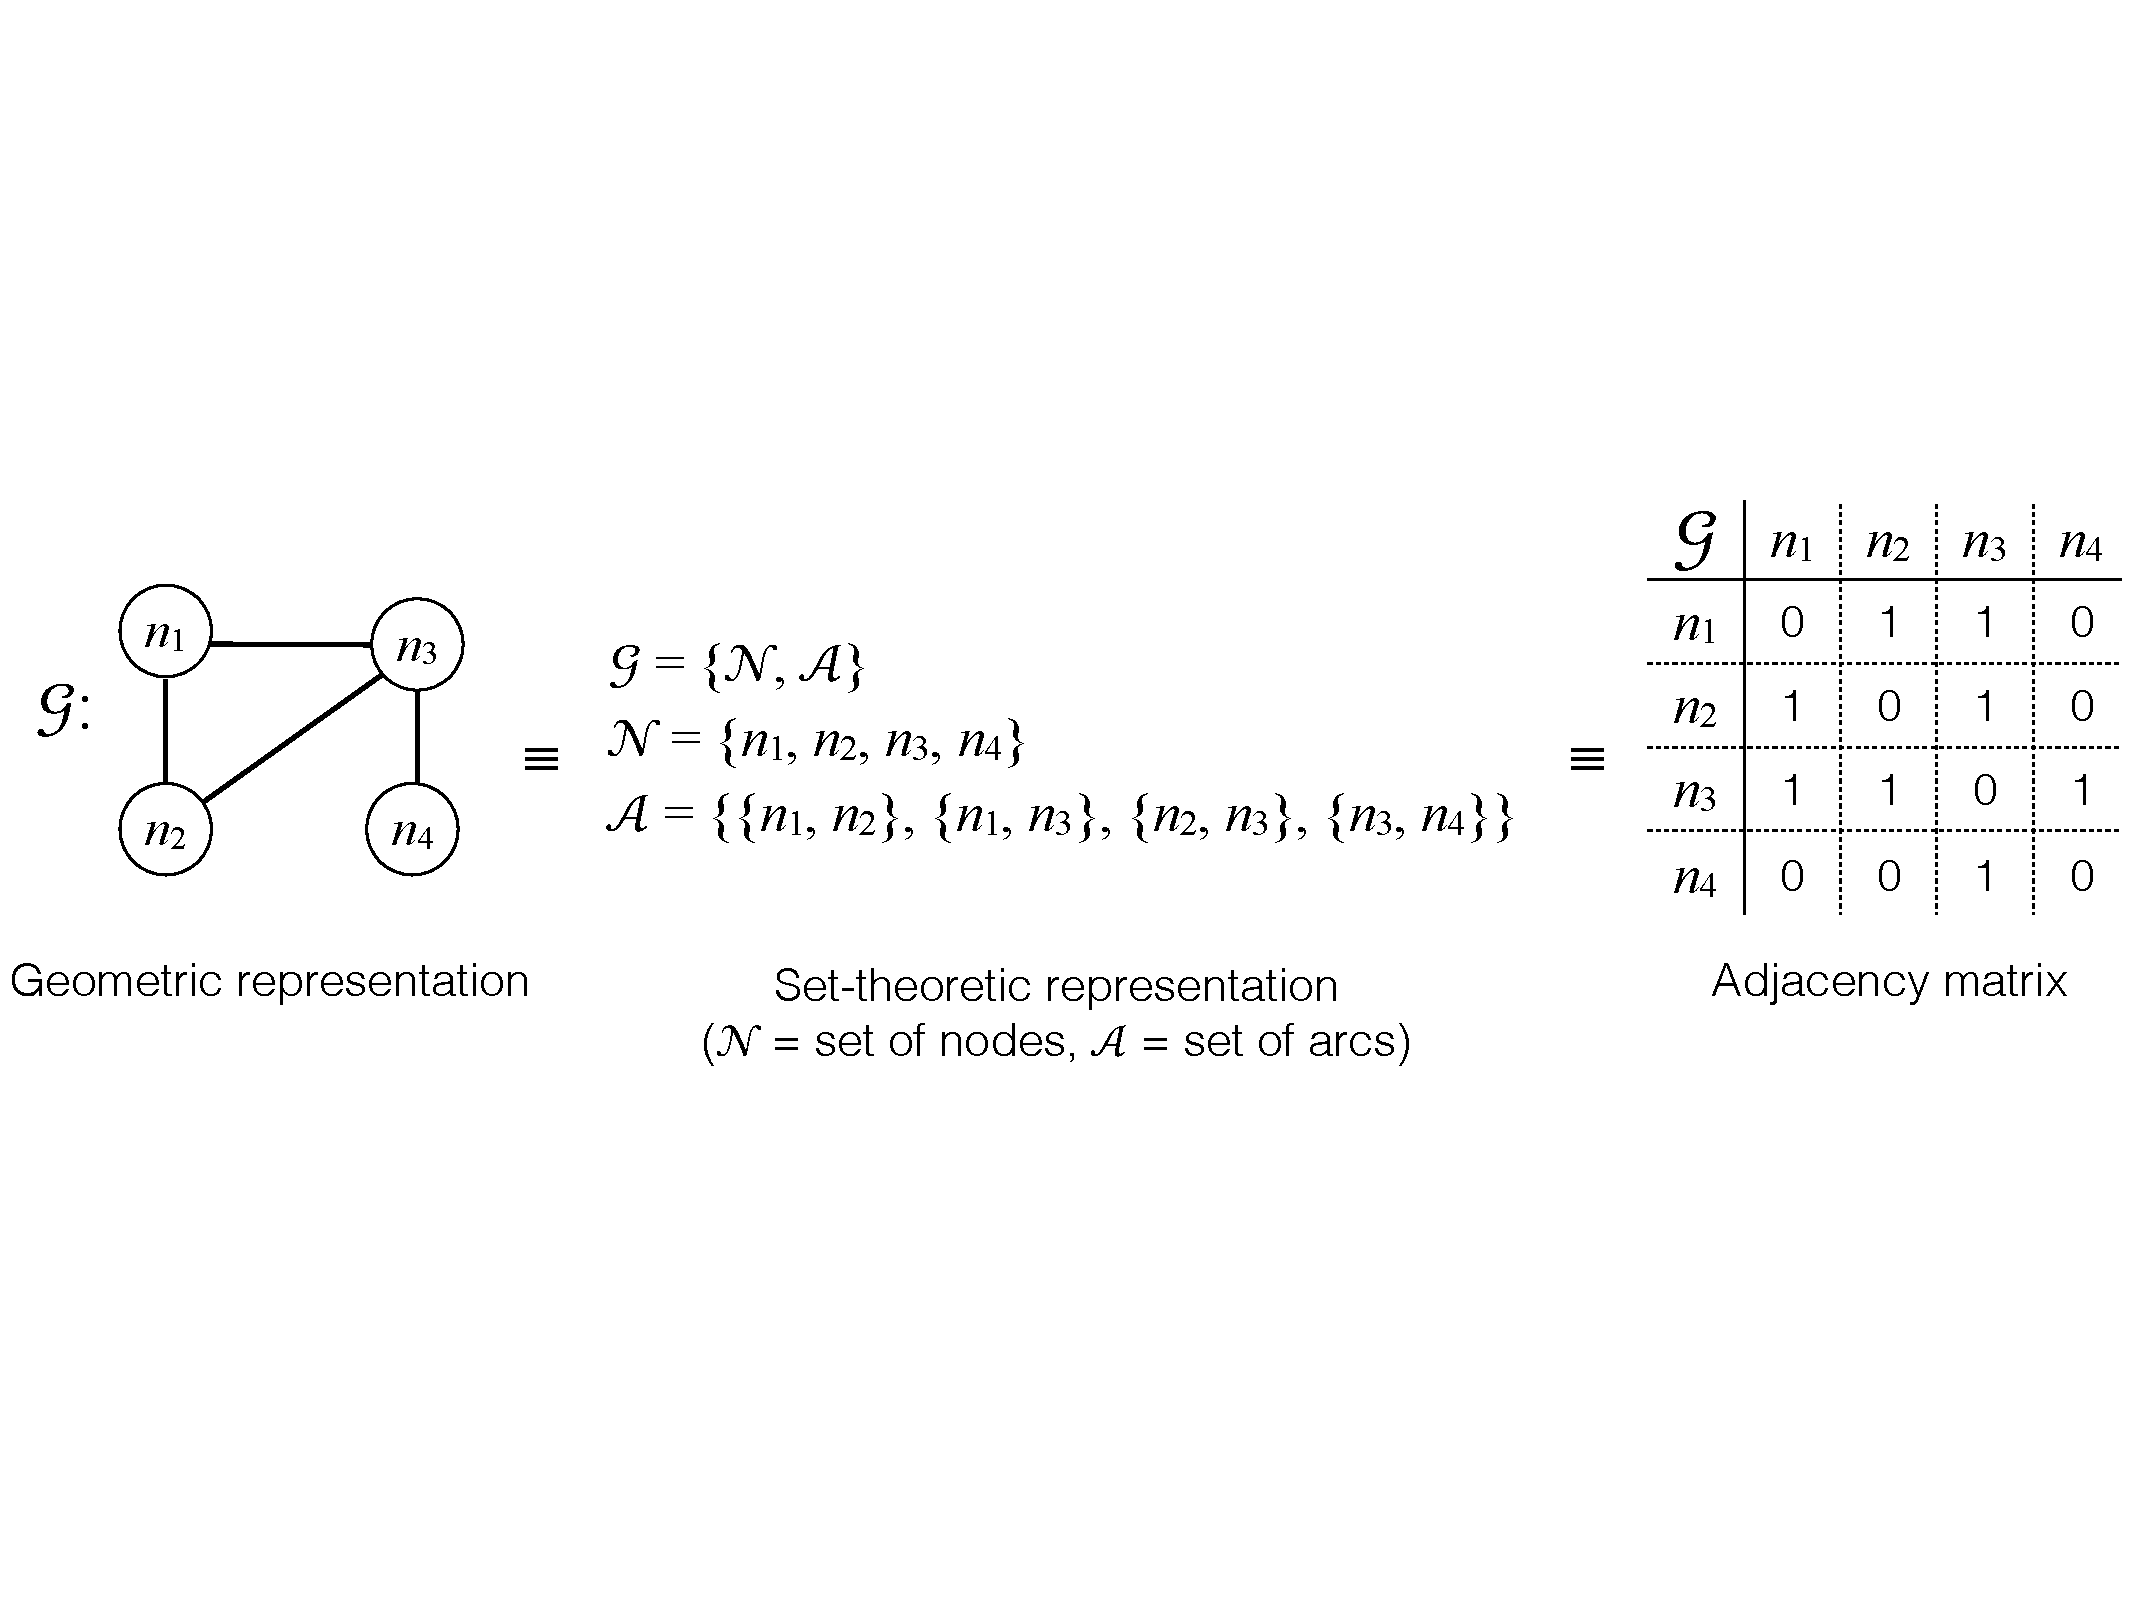
\includegraphics[width=\linewidth]{Fig/LexicalNetworks/undirectedGrapRep.pdf}
\caption{Three modes of representing a given undirected graph $\mathcal{G}$}\label{fig:undirectedGrapRep}
\end{figure}

The \notion{geometric representation}\index[notion]{graph!geometric representation of a \tld} is almost self-explanatory. In our figure, we put node names inside the circles representing nodes in order to highlight the fact that such names are only node IDs, and not attributes of the nodes.\footnote{This is in reference to what was said earlier about the distinction we maintain between the terms \textit{network} and \textit{graph} (network stripped of non-structural information).} A graph is entirely defined by its \notion{topology}\index[notion]{topology|emph}\index[notion]{graph!topology of a \tld|emph}\phantomsection\label{txt:topology}: its system of nodes and connecting arcs. Consequently, in a graph geometric representation, the spacial distribution\index[notion]{node of a network\slashs{}graph!geometric distribution of \tlds}\index[notion]{geometric distribution of graph nodes} of nodes and arcs is irrelevant from a formal point of view and only serves legibility purposes.\footnote{We will show (\sectref{sec:lexicalProximityTopologicalProximity}, p.\thinspace\pageref{sec:lexicalProximityTopologicalProximity}) that geometric distribution of nodes can nonetheless be used to encode additional information about the graph's overall topology.} The relative positioning of nodes in the geometric representation of \figref{fig:undirectedGrapRep} can be totally upended (\textit{n}\tsub{4} at the very top, \textit{n}\tsub{1} below \textit{n}\tsub{3}, \textit{n}\tsub{2} positioned much closer to \textit{n}\tsub{3}, etc.); it will remain the representation of the same graph $\mathcal{G}$ as long as connections established by the arcs remain identical.

The \notion{set-theoretic representation}\index[notion]{graph!set-theoretic representation of a \tld} defines a graph as a mathematical set comprised of two subsets: (i)~a set of nodes and (ii)~a set of arcs; this latter set contains unordered two-element sets encoding non-oriented binary relations between nodes.

The \notion{adjacency matrix}\index[notion]{adjacency matrix (of a graph)}\index[notion]{graph!adjacency matrix of a \tld} is a table where each row and each column correspond to a node of the graph; each cell of the table indicates whether an arc connects the corresponding nodes: \textsf{1} means that the nodes are connected and \textsf{0} means that they are not. The adjacency matrix for graph $\mathcal{G}$ (\figref{fig:undirectedGrapRep}) is symmetrical\index[notion]{adjacency matrix (of a graph)!(non-)symmetrical \tld} relative to the table's top-left to bottom-right diagonal; this comes from the fact that, the arcs being non-oriented, any \textit{n}---\textit{n}′ arc is equally an \textit{n}′---\textit{n} arc.

We exemplified the three modes of representation above with an undirected graph for pedagogical purposes. However, lexical relations examined earlier in \sectref{sec:mainCharacteristicsLS} are all oriented and, therefore, the graphs underlying Lexical Systems\index[notion]{graph!Lexical System \tld}\index[notion]{Lexical System!\tld\ graph} are \notion{directed graphs}\index[notion]{graph!directed \tld}. \figref{fig:directedGrapRep} gives the three representations of a directed graph $\mathcal{G}^\prime$.

\begin{figure}

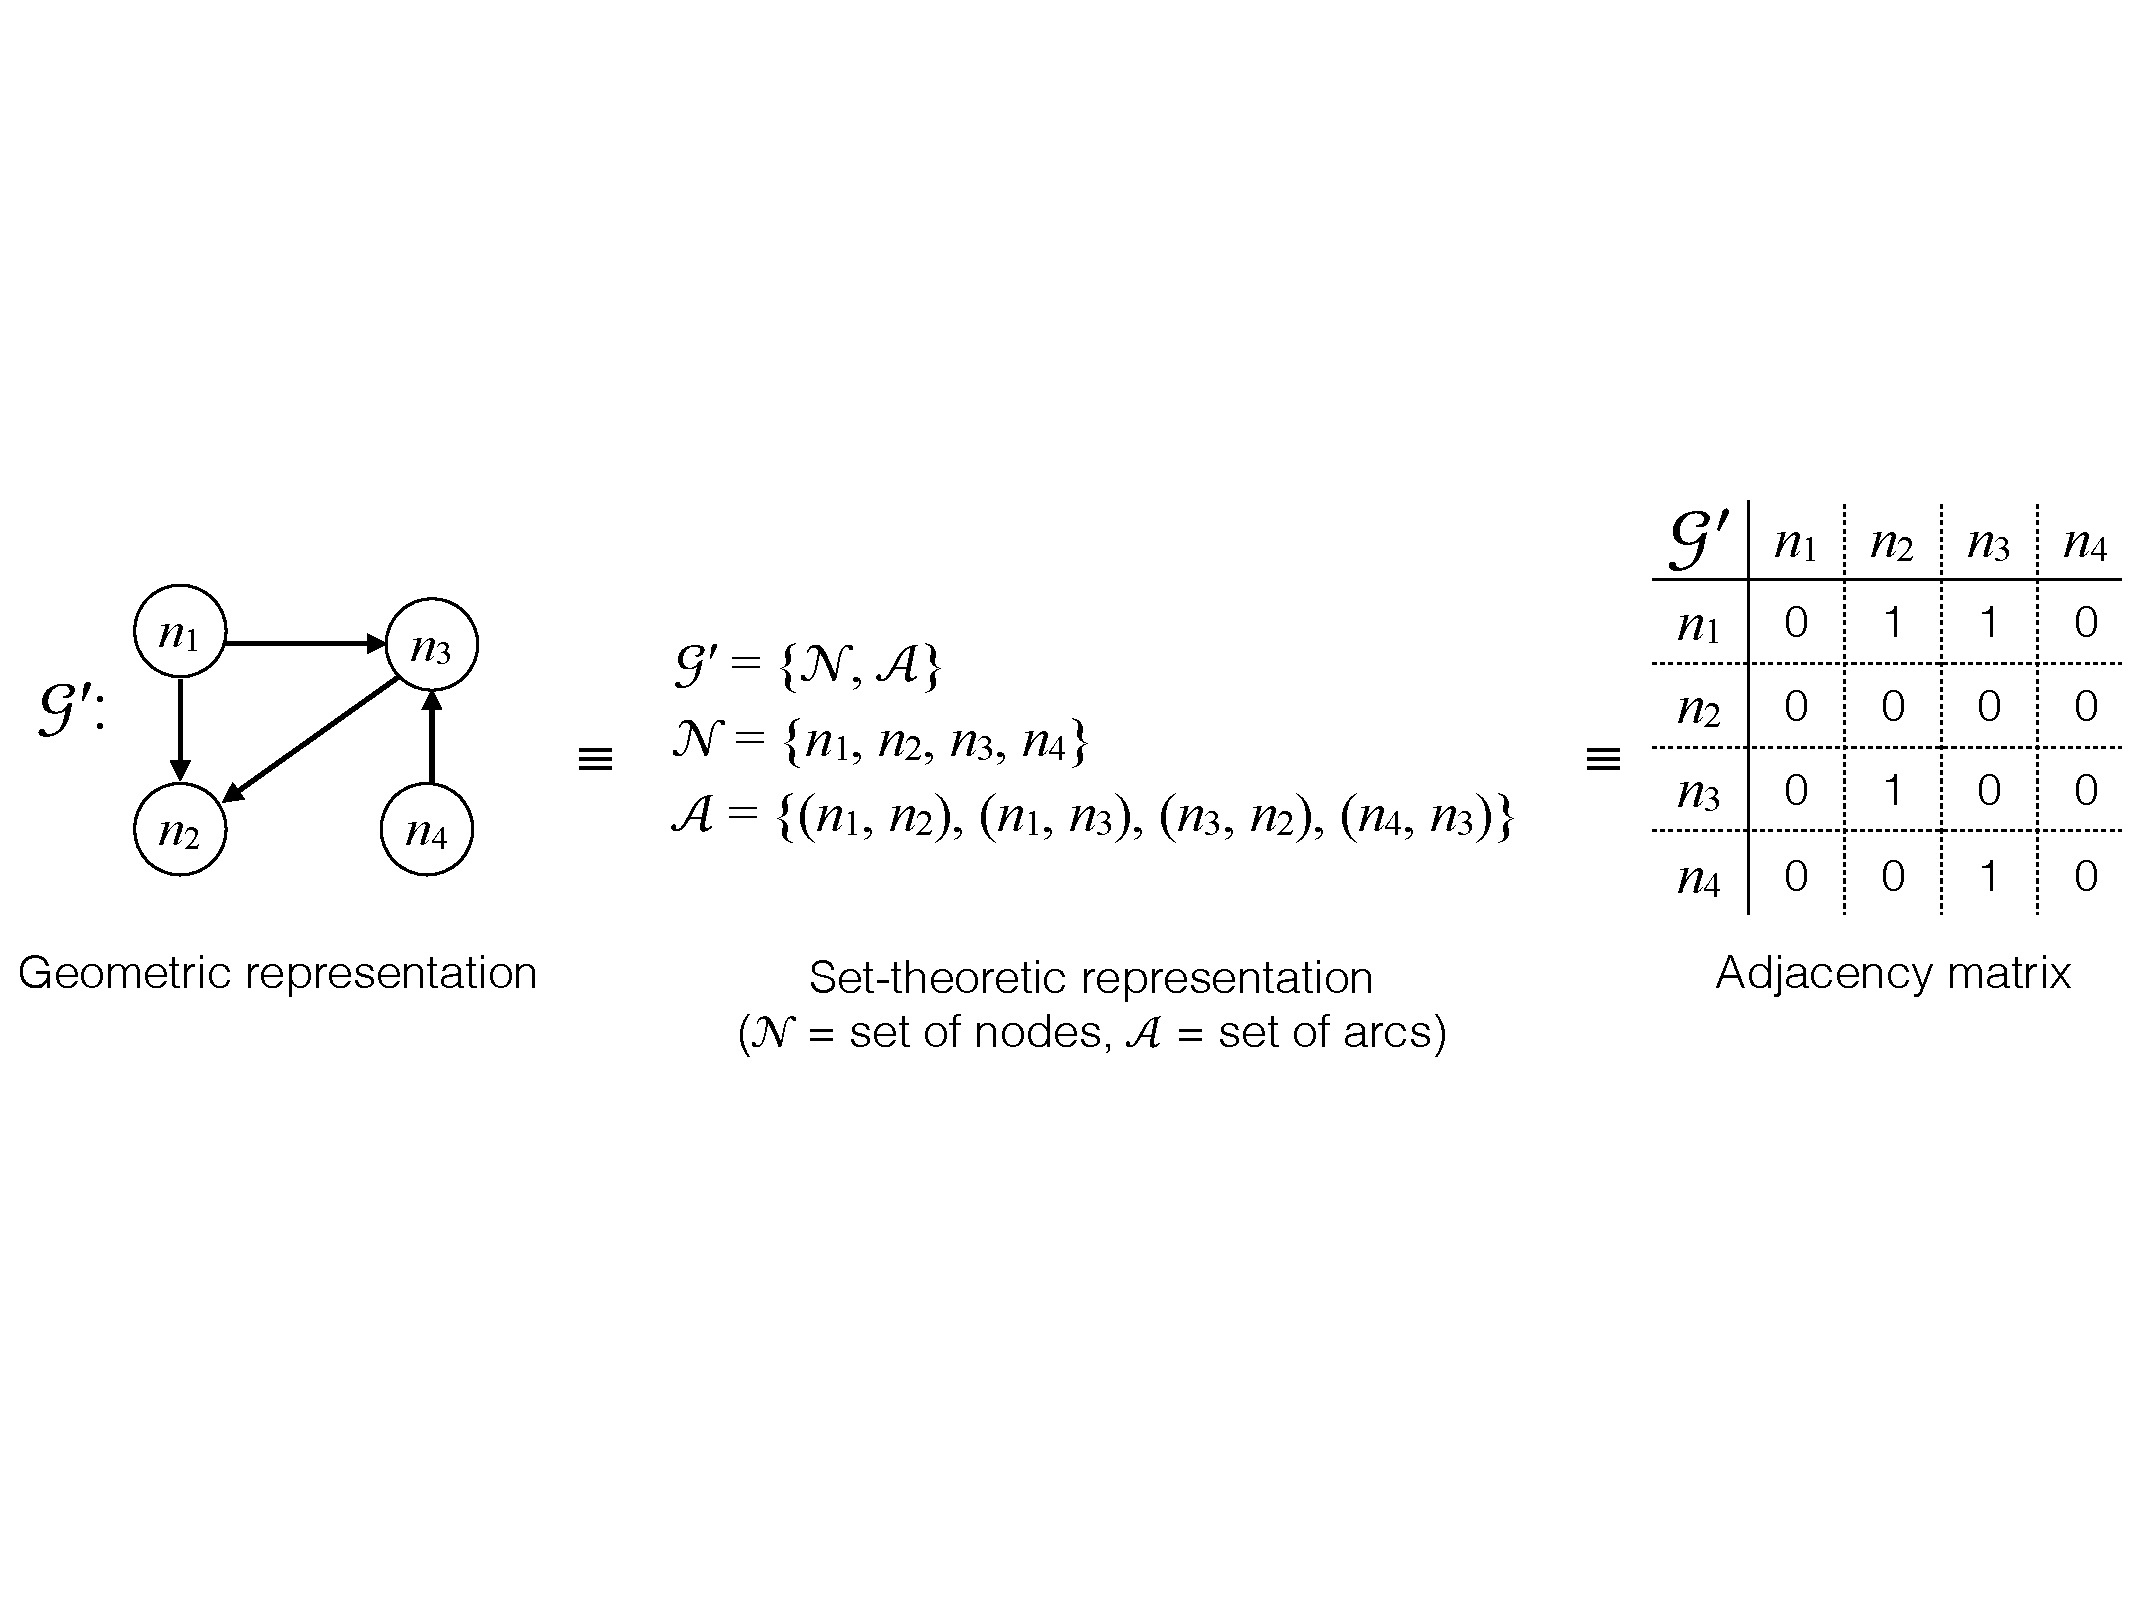
\includegraphics[width=\linewidth]{Fig/LexicalNetworks/directedGrapRep.pdf}
\caption{Three modes of representing a given directed graph $\mathcal{G}^\prime$}\label{fig:directedGrapRep}
\end{figure}

%https://medium.com/basecs/from-theory-to-practice-representing-graphs-cfd782c5be38
Differences with the representations of \figref{fig:undirectedGrapRep} (an undirected graph) are as follows:

\begin{itemize}

\item arcs of the geometric representations are \emph{arrows}\index[notion]{arrow of a network\slashs{}graph [=~arc]}\index[notion]{network \lfgp{see also \textit{graph}}!arrow of a \tld} -- they indicate the \notion{starting node} and the \notion{end node}\index[notion]{node of a network\slashs{}graph!starting\slashs{}end \tld} for each relation;

\item the set of arcs $\mathcal{A}$ in the set-theoretic representation contains (ordered) \mbox{\emph{couples}} of nodes -- instead of (unordered) two-element sets of nodes;

\item \textsf{1}s and \textsf{0}s in the adjacency matrix take into account, for each cell, which node is the starting node and which node is the end node of the corresponding relation; note that the adjacency matrix of graph $\mathcal{G}^\prime$ is non-symmetrical\index[notion]{adjacency matrix (of a graph)!(non-)symmetrical \tld}.

\end{itemize}

One of the advantages of the geometric representation of graphs over the two other representations is that it offers a clear visualization of possible paths between nodes. A \notion{path}\index[notion]{path in a graph\slashs{}network|emph}\index[notion]{graph!path in a \tld|emph}\phantomsection\label{txt:pathInAGraph} in a graph is a sequence of arcs that connects a sequence of nodes where neither arcs nor nodes are repeated. In an oriented graph, one can consider \notion{directed paths}\index[notion]{path in a graph\slashs{}network!directed \tld} -- the sequence of arcs follows the orientation of the arcs -- or \notion{undirected paths}\index[notion]{path in a graph\slashs{}network!undirected \tld} -- the orientation of arcs is not relevant. For instance, the geometric representation of \figref{fig:directedGrapRep} clearly shows:

\begin{itemize}

\item two directed paths from \textit{n}\tsub{1} to \textit{n}\tsub{2}, namely: \textit{n}\tsub{1}-\textit{n}\tsub{2} and \textit{n}\tsub{1}-\textit{n}\tsub{3}-\textit{n}\tsub{2};

\item two undirected paths from \textit{n}\tsub{1} to \textit{n}\tsub{4}, namely: \textit{n}\tsub{1}-\textit{n}\tsub{3}-\textit{n}\tsub{4} and \textit{n}\tsub{1}-\textit{n}\tsub{2}-\textit{n}\tsub{3}-\textit{n}\tsub{4}.

\end{itemize}

The notion of path is central in the definition of small-world networks\index[notion]{network \lfgp{see also \textit{graph}}!small-world \tld}\index[notion]{small-world!\tld\ network} (see \sectref{sec:smallWorldNetworks}, p.\thinspace\pageref{sec:smallWorldNetworks}).

\subsubsubsection{Structural properties of Lexical System graphs}

Graphs are characterized by structural properties\index[notion]{graph!structural property of a \tld} that pertain, primarily, (i)~to the nature of their arcs -- for instance, we have already established that we are concerned here with directed graphs only -- and (ii)~to the types of node-arc configurations they contain. We concentrate on \notion{Lexical System graphs}\index[notion]{graph!Lexical System \tld|emph}\index[notion]{Lexical System!\tld\ graph|emph} -- referred to as $\mathcal{G}_{LS}$ -- and identify four properties (A--D) that characterize them as a specific type of directed graph\index[notion]{graph!directed \tld}. These properties are listed below, then summarized and exemplified in \figref{fig:propertiesOfGLS} (p.\thinspace\pageref{fig:propertiesOfGLS}).

\begin{enumerate}

\item[A)] Labeled graph.\enskip\index[notion]{graph!labeled \tld}Each arc of a $\mathcal{G}_{LS}$ is defined by a starting node, an end node and a \notion{label}\index[notion]{label of a network\slashs{}graph arc} that identifies the lexical relation encoded by the arc: LF relation, copolysemy relation, etc. This characterizes a $\mathcal{G}_{LS}$ as an oriented \notion{labeled graph}.

\item[B)] Weighed graph.\enskip\index[notion]{graph!weighed \tld}When presenting LF and non-LF relations encoded in Lexical Systems, we have indicated that these relations can be distinguished according to their semantic weight\index[notion]{semantic!\tld\ weight}\index[notion]{weight, semantic} (\sectref{sec:LFRelationsBackboneOfLFs}, p.\thinspace\pageref{par:semanticWeightLFRelation}). This information is encoded in a $\mathcal{G}_{LS}$ for each arc of the graph, concurrently with the arc label, which characterizes a $\mathcal{G}_{LS}$ as a \notion{weighed graph}.

\item[C)] Multigraph.\enskip\index[notion]{graph!multi\tld}Two nodes of a $\mathcal{G}_{LS}$ can be connected by more than one arc -- for instance, when two lexical units are connected simultaneously by an LF relation and a meaning-inclusion relation\index[notion]{lexical relation!meaning-inclusion \tld}\index[notion]{relation!meaning-inclusion \tld}\index[notion]{meaning!\tld\ inclusion relation}, as in \Next. This results in \notion{multiple arcs}\index[notion]{arc of a network\slashs{}graph!multiple \tlds} in a $\mathcal{G}_{LS}$, which characterizes it as a \notion{multigraph}.

\begingroup
\small

\ex. \setlength{\tabcolsep}{2pt}
\begin{tabular}[t]{ l l >{\raggedright\arraybackslash}p{7cm} }
\lfappl{Gener}{\textit{gas}\tsub{(N)}} & = & \textit{substance} \\*
\multicolumn{3}{l}{\textsc{gas}\tsub{(N)}\thinspace\lexRel{meaning inclusion}\thinspace\textsc{substance}} \\*
\multicolumn{3}{l}{\lfgp{Where `substance' is the central component in the definition of \textsc{gas}\tsub{(N)}}}
\end{tabular}

\endgroup\index[lf]{Gener@\lf{Gener}}\index[notion]{component of a definition!central \tld}\index[notion]{definition!central component of a \tld}

\item[D)] Cyclic graph.\enskip\index[notion]{graph!cyclic \tld}A $\mathcal{G}_{LS}$ contains \notion{cycles}\index[notion]{cycle in a graph\slashs{}network}\index[notion]{graph!cycle in a \tld}, i.e., directed paths\index[notion]{path in a graph\slashs{}network!directed \tld} that originate and end at the same given node. This characterizes a $\mathcal{G}_{LS}$ as a \notion{cyclic graph}. For instance, the set of LF relations in \Next is encoded as a two-step cycle in the corresponding $\mathcal{G}_{LS}$.

\begingroup
\small

\ex. \setlength{\tabcolsep}{2pt}
\begin{tabular}[t]{ l l >{\raggedright\arraybackslash}p{7cm} }
\lfappl{S\tsub{0}}{\textit{present}\tsub{(V)}} & = & \textit{presentation} \\*
\lfappl{V\tsub{0}}{\textit{presentation}} & = & \textit{present}\tsub{(V)}
\end{tabular}

\endgroup\index[lf]{S0@\lf{S\tsub{0}}}\index[lf]{V0@\lf{V\tsub{0}}}

The cycle in \Last also corresponds to a multigraph configuration -- see property C) above.

\end{enumerate}

The above four properties are recapitulated in \figref{fig:propertiesOfGLS}, with illustrations that apply to several properties wherever it is convenient to do so.

\begin{figure}

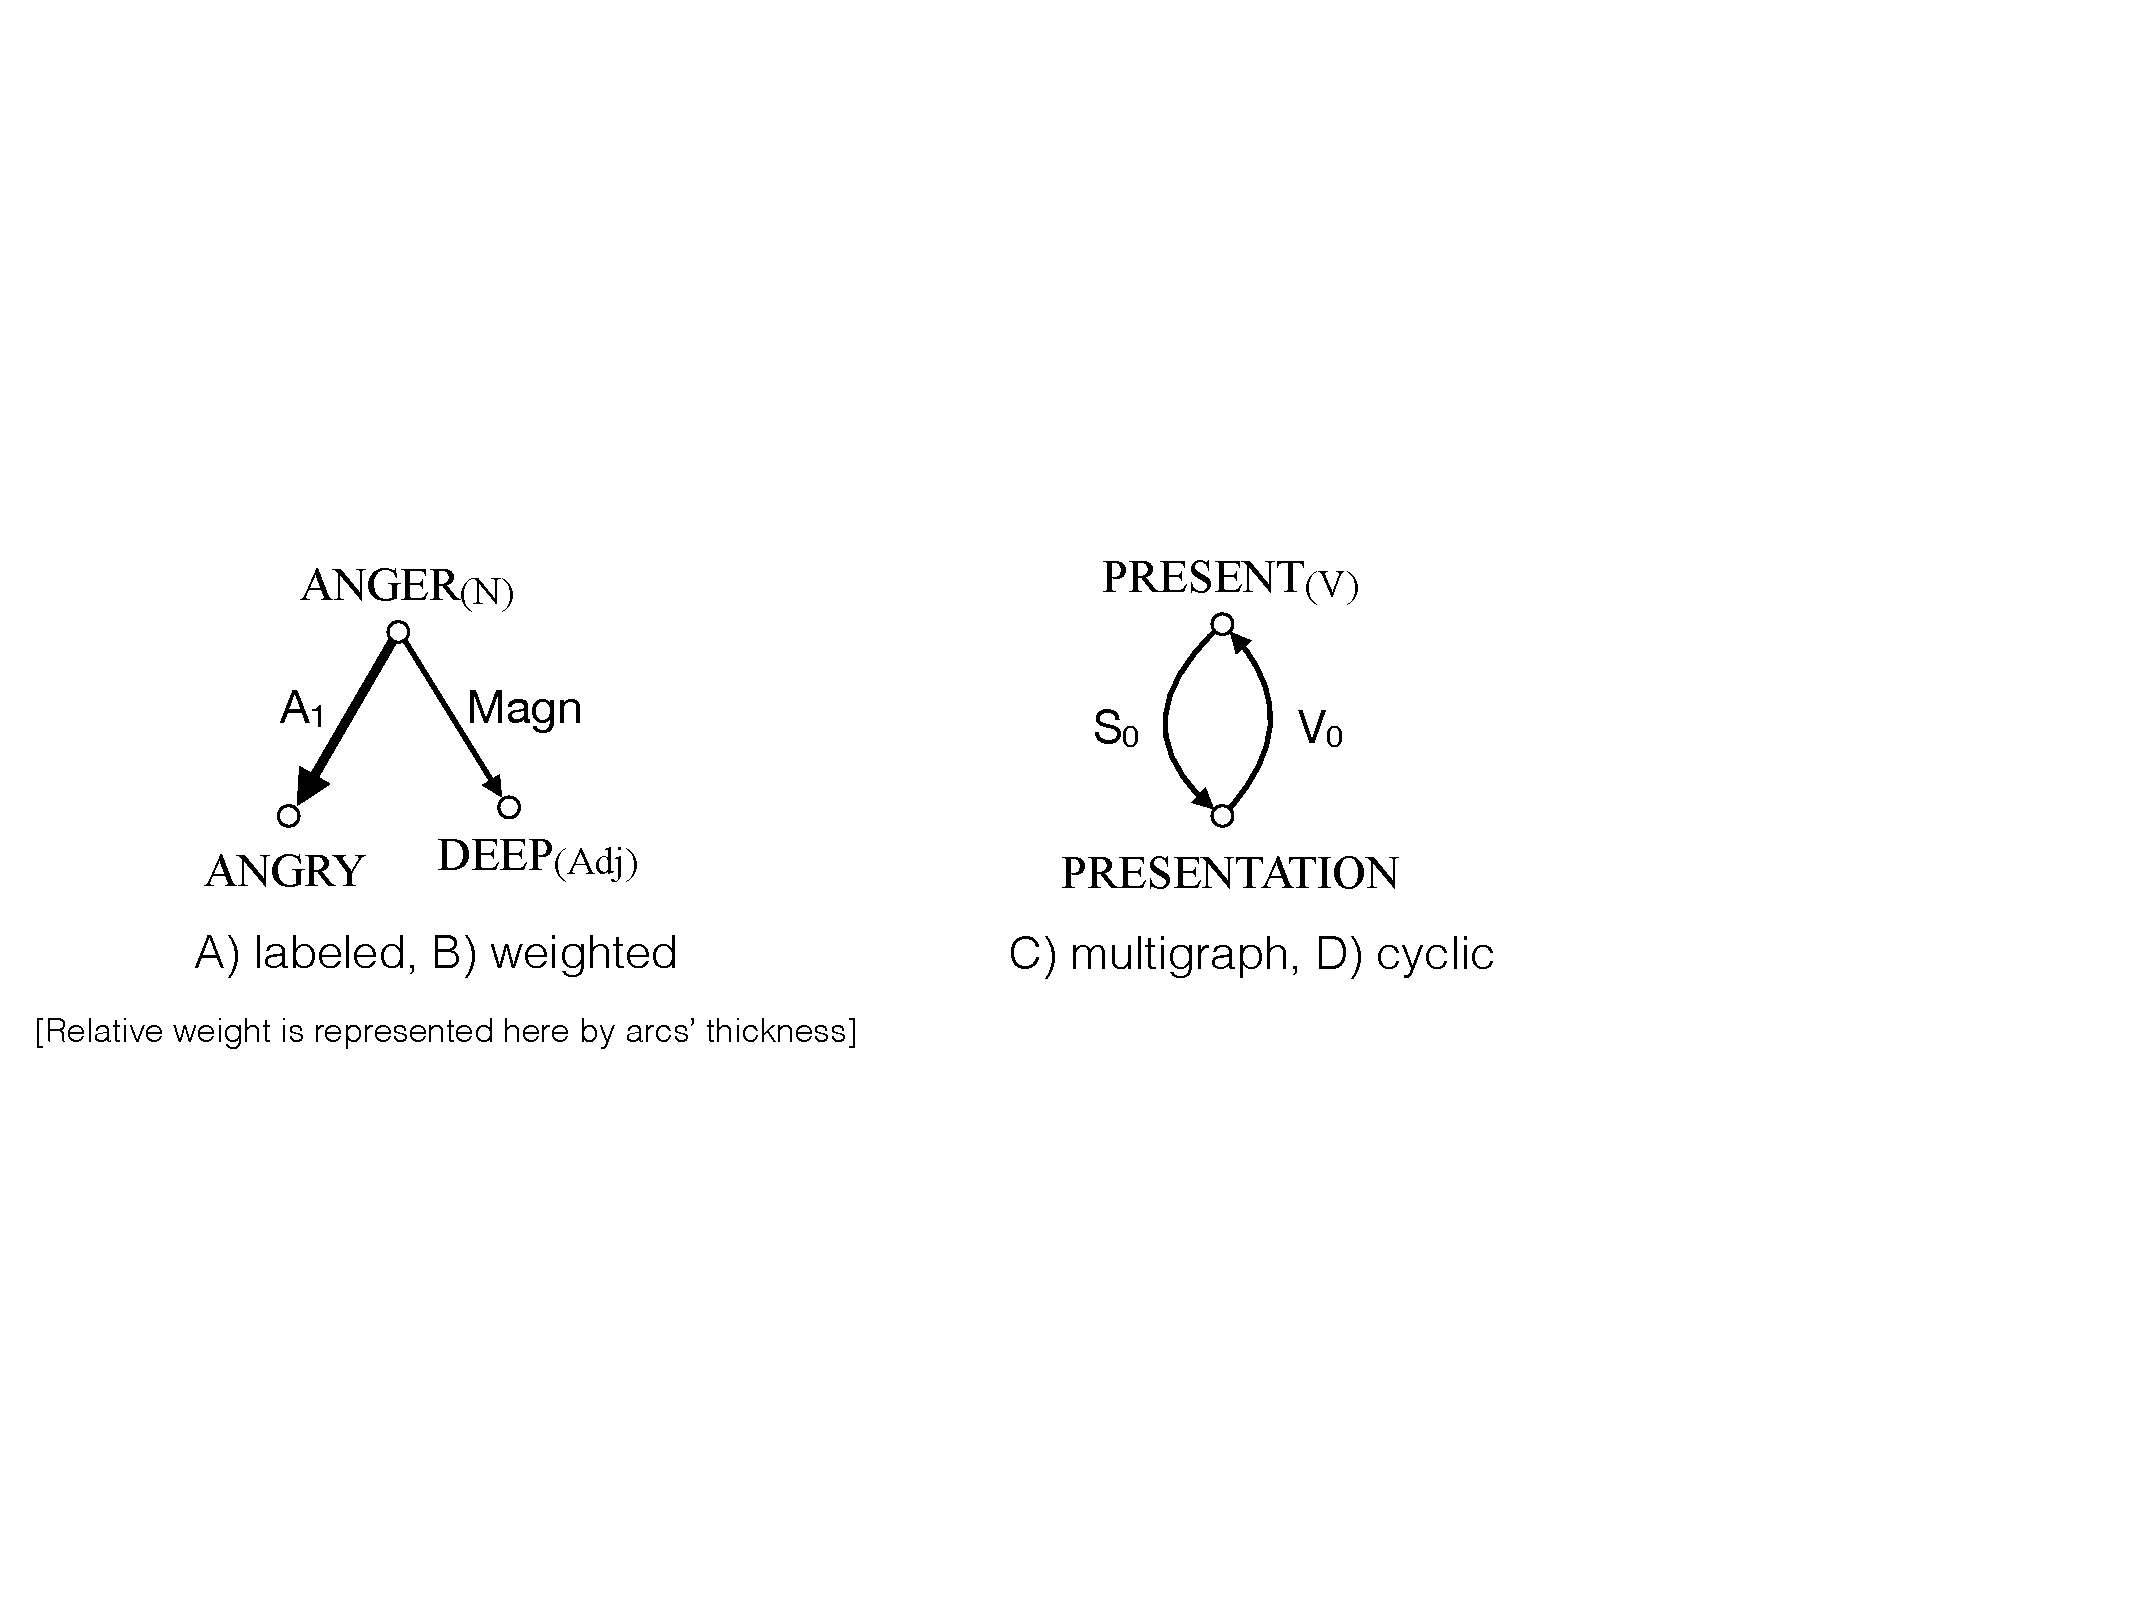
\includegraphics[width=0.8\linewidth]{Fig/LexicalNetworks/propertiesOfGLS.pdf}
\caption{Four structural properties of a Lexical System graph $\mathcal{G}_{LS}$}\label{fig:propertiesOfGLS}
\end{figure}

\subsubsubsection{Lexical Systems as small-world networks}\label{sec:smallWorldNetworks}

The properties examined above characterize a $\mathcal{G}_{LS}$ at a \notion{microscopic} level\index[notion]{microscopic structure (of a graph)}, i.e., at the level of individual nodes and relations they participate in. We are now taking a bird's-eye view of such graphs in order to contrast their microscopic and \notion{macroscopic}\index[notion]{macroscopic structure (of a graph)}\index[notion]{graph!microscopic vs. macroscopic structure of a \tld} structures. For this, we focus on a natural law that tends to apply to all real-world networks\index[notion]{real-world network\slashs{}graph}\index[notion]{network \lfgp{see also \textit{graph}}!real-world \tld} (as characterized in \sectref{sec:basicsGraphTheory}, p.\thinspace\pageref{sec:basicsGraphTheory}).

\begin{soundboxnotitle}
Graph theory\index[notion]{graph!\tld\ theory} has determined that graphs of real-world networks have characteristic topological\index[notion]{topology}\index[notion]{graph!topology of a \tld} properties that identify them as \notion{small-world} \mbox{\textit{networks}}\index[notion]{network \lfgp{see also \textit{graph}}!small-world \tld|emph}\index[notion]{small-world!\tld\ network|emph} \parencite{WattsStrogatz1998}.
\end{soundboxnotitle}

The term \emph{small-world network} refers to the small-world phenomenon\index[notion]{small-world!\tld\ phenomenon} in social networks,\footnote{By \textit{social network}, we mean here social structures made up of individuals having social interactions. We are not referring to social media platforms on the Internet.} which can be presented as follows: there is a high probability for any two randomly selected individuals $i_1$ and $i_2$ to be connected through a relatively short chain of acquaintances \parencite[163]{Kleinberg2000} -- hence the expression \textit{It's a small world!} Though this phenomenon was originally conceptualized from the perspective of social and psychological studies \parencite{Milgram1967}, it is a characteristic feature of real-world networks of any kind. The topological structure of a small-world network has (at least) the four properties (A--D) described below; in order to anchor what follows more directly to our topic of interest (i.e., Lexical Systems), these properties are introduced as properties of a given $\mathcal{G}_{LS}$.\footnote{We try to keep what follows as little mathematical as possible, at the expense of accuracy. See \textcite{GaumeEtAl2010} for a purely mathematical characterization of lexical graphs as small-world networks; see \textcite[Sec.~3]{GaderEtAl2014a-e} for the measurement of the \textit{pedigree} of Lexical Systems as small-world networks.}

\begin{enumerate}

\item[A)] Mainly connected graph.\enskip\index[notion]{graph!(dis)connected \tld}A $\mathcal{G}_{LS}$ may contain some isolated tiny subgraphs (possibly, isolated nodes); however, the bulk of its structure forms one huge \notion{connected graph}: a graph in which there exists at least one path\index[notion]{path in a graph\slashs{}network}\index[notion]{graph!path in a \tld} connecting any two nodes.

\item[B)] Sparse graph.\enskip\index[notion]{graph!sparse \tld}The arc-to-node ratio in a $\mathcal{G}_{LS}$ is low: there are more arcs than nodes, but the difference is not drastic. Consequently, there is an extremely low probability for any two nodes in a $\mathcal{G}_{LS}$ to be \emph{directly} connected. This characterizes a $\mathcal{G}_{LS}$ as a \notion{sparse graph}.\footnote{\label{fn:nodeDegree}The mathematical measurement used to evaluate this sparsity is the \emph{average node degree} of the graph (the average number of arcs connected to each node) -- for lexical networks, see \textcite[Sec.~2]{GaumeEtAl2010}.}

\item[C)] It's a small world, nonetheless!\enskip In spite of its sparsity, a $\mathcal{G}_{LS}$ displays the small-world phenomenon in the sense that any two nodes of $\mathcal{G}_{LS}$, no matter how distant they may be in the topological structure of the graph, are connected by at least one relatively short path. This phenomenon is mainly made possible by two factors.

First, though most nodes of $\mathcal{G}_{LS}$ are weakly connected, there are nodes that function as lexical hubs from a relational viewpoint; for instance:

\begin{itemize}

\item generic terms\index[notion]{generic term} that identify large lexical classes (\textsc{animal}, \textsc{vehicle}, \textsc{feeling}, ...) and thus are ending nodes\index[notion]{node of a network\slashs{}graph!starting\slashs{}end \tld} of many \lf{Gener} arcs\index[lf]{Gener@\lf{Gener}};
\item collocative lexical units\index[notion]{lexical unit!collocative \tld} forming collocations\index[notion]{collocation!base of a \tld} with a large spectrum of potential bases\index[notion]{base!\tld\ of a collocation} -- for instance, the \lf{Magn}\index[lf]{Magn@\lf{Magn}} value \textsc{heavy}\tsub{(Adj)}\sensenum{2} mentioned in \sectref{sec:LFRelationsBackboneOfLFs}, p.\thinspace\pageref{txt:HEAVY-Adj-2}.

\end{itemize}

Second, many copolysemy\index[notion]{polysemy!co\tld}\index[notion]{copolysemy}\index[notion]{lexical relation!copolosemy \tld}\index[notion]{relation!copolysemy \tld} and idiom-component relations\index[notion]{lexical relation!idiom-component \tld}\index[notion]{relation!idiom-component \tld}\index[notion]{idiom!\tld-component relation} in a $\mathcal{G}_{LS}$ establish direct paths between semantic areas that are otherwise very far apart; for instance:

\begin{itemize}

\item \lu{crane}{(N)}{}{I} \lfgp{animals}\thinspace\lexRel{copolysem. metaphor}\thinspace\lu{crane}{(N)}{}{II} \lfgp{machines};

\item \idiom{\textsc{go bananas}} \lfgp{feelings\slashs{}behaviors}\thinspace\lexRel{idiom-comp.}\thinspace\textsc{banana} \lfgp{fruits}.

\end{itemize}

\item[D)] High clustering rate.\enskip\phantomsection\label{par:highClusteringRate}A $\mathcal{G}_{LS}$ is sparse at a macroscopic level\index[notion]{macroscopic structure (of a graph)} but dense at a microscopic level\index[notion]{microscopic structure (of a graph)}\index[notion]{graph!microscopic vs. macroscopic structure of a \tld}, where a profusion of small node clusters\index[notion]{cluster of nodes in a graph}\index[notion]{node of a network\slashs{}graph!cluster of \tlds} are found. In mathematical terms, a $\mathcal{G}_{LS}$ has a high \notion{clustering rate}\index[notion]{cluster of nodes in a graph!clustering rate|emph}\index[notion]{graph!clustering rate of a \tld|emph}: there is a much higher probability for two nodes \textit{n}\tsub{1} and \textit{n}\tsub{2} to be directly connected if both of them are directly connected to a node \textit{n}\tsub{3} than if they are randomly selected. This is easily illustrated with LF relations, where various clustering \notion{inference rules}\index[notion]{inference rule} such as \Next and \NNext can be established. \figref{fig:LFClusters} visualizes linguistic illustrations given in \Next and \NNext.

\begingroup
\small

\ex.\label{ex:clusteringInfRule1} \emph{If} \lfappl{f}{L} = L′\textbf{,} L′′ \\*
         \emph{then} there exists \lfappl{Syn\slashs{}Syn\tsub{$\supset$}\slashs{}Syn\tsub{$\subset$}\slashs{}Syn\tsub{$\cap$}}{L′} = L′′;\footnote{This is true because all the elements of an LF value must be (quasi-)synonymous.} for instance:\\*
\textbullet\hspace{2pt} \lfappl{S\tsub{2}}{\textit{married}} = \textit{spouse}\tsub{(N)}\textbf{,} \idiom{\textit{better half}}\\*
\textbullet\hspace{2pt} \lfappl{Syn\tsub{$\cap$}}{\textit{spouse}\tsub{(N)}} = \idiom{\textit{better half}}

\endgroup\index[lf]{Si@\lf{S\tsub{i}}!\lf{S\tsub{2}}}\index[lf]{Syn@\lf{Syn}!\lf{Syn\tsub{$\cap$}}}

\begingroup
\small

\ex.\label{ex:clusteringInfRule2} \emph{If} \lfappl{f\tsub{1}}{L} = L′ \emph{and} \lfappl{f\tsub{2}}{L′} = L′′ \\*
         \emph{then} there is an above-average probability that there exists \lfappl{f\tsub{3}}{L} = L′′; \\* for instance:\\*
\textbullet\hspace{2pt} \lfappl{Conv\tsub{21}}{\textit{defeat}\tsub{(N)}} = \textit{victory} and \lfappl{A\tsub{1}}{\textit{victory}} = \textit{victorious}\\*
\textbullet\hspace{2pt} \lfappl{A\tsub{2}}{\textit{defeat}\tsub{(N)}} = \textit{victorious}

\endgroup\index[lf]{Convijk@\lf{Conv\tsub{ijk}}!\lf{Conv\tsub{21}}}\index[lf]{Ai@\lf{A\tsub{i}}!\lf{A\tsub{1}}}\index[lf]{Ai@\lf{A\tsub{i}}!\lf{A\tsub{2}}}

\end{enumerate}

\begin{figure}

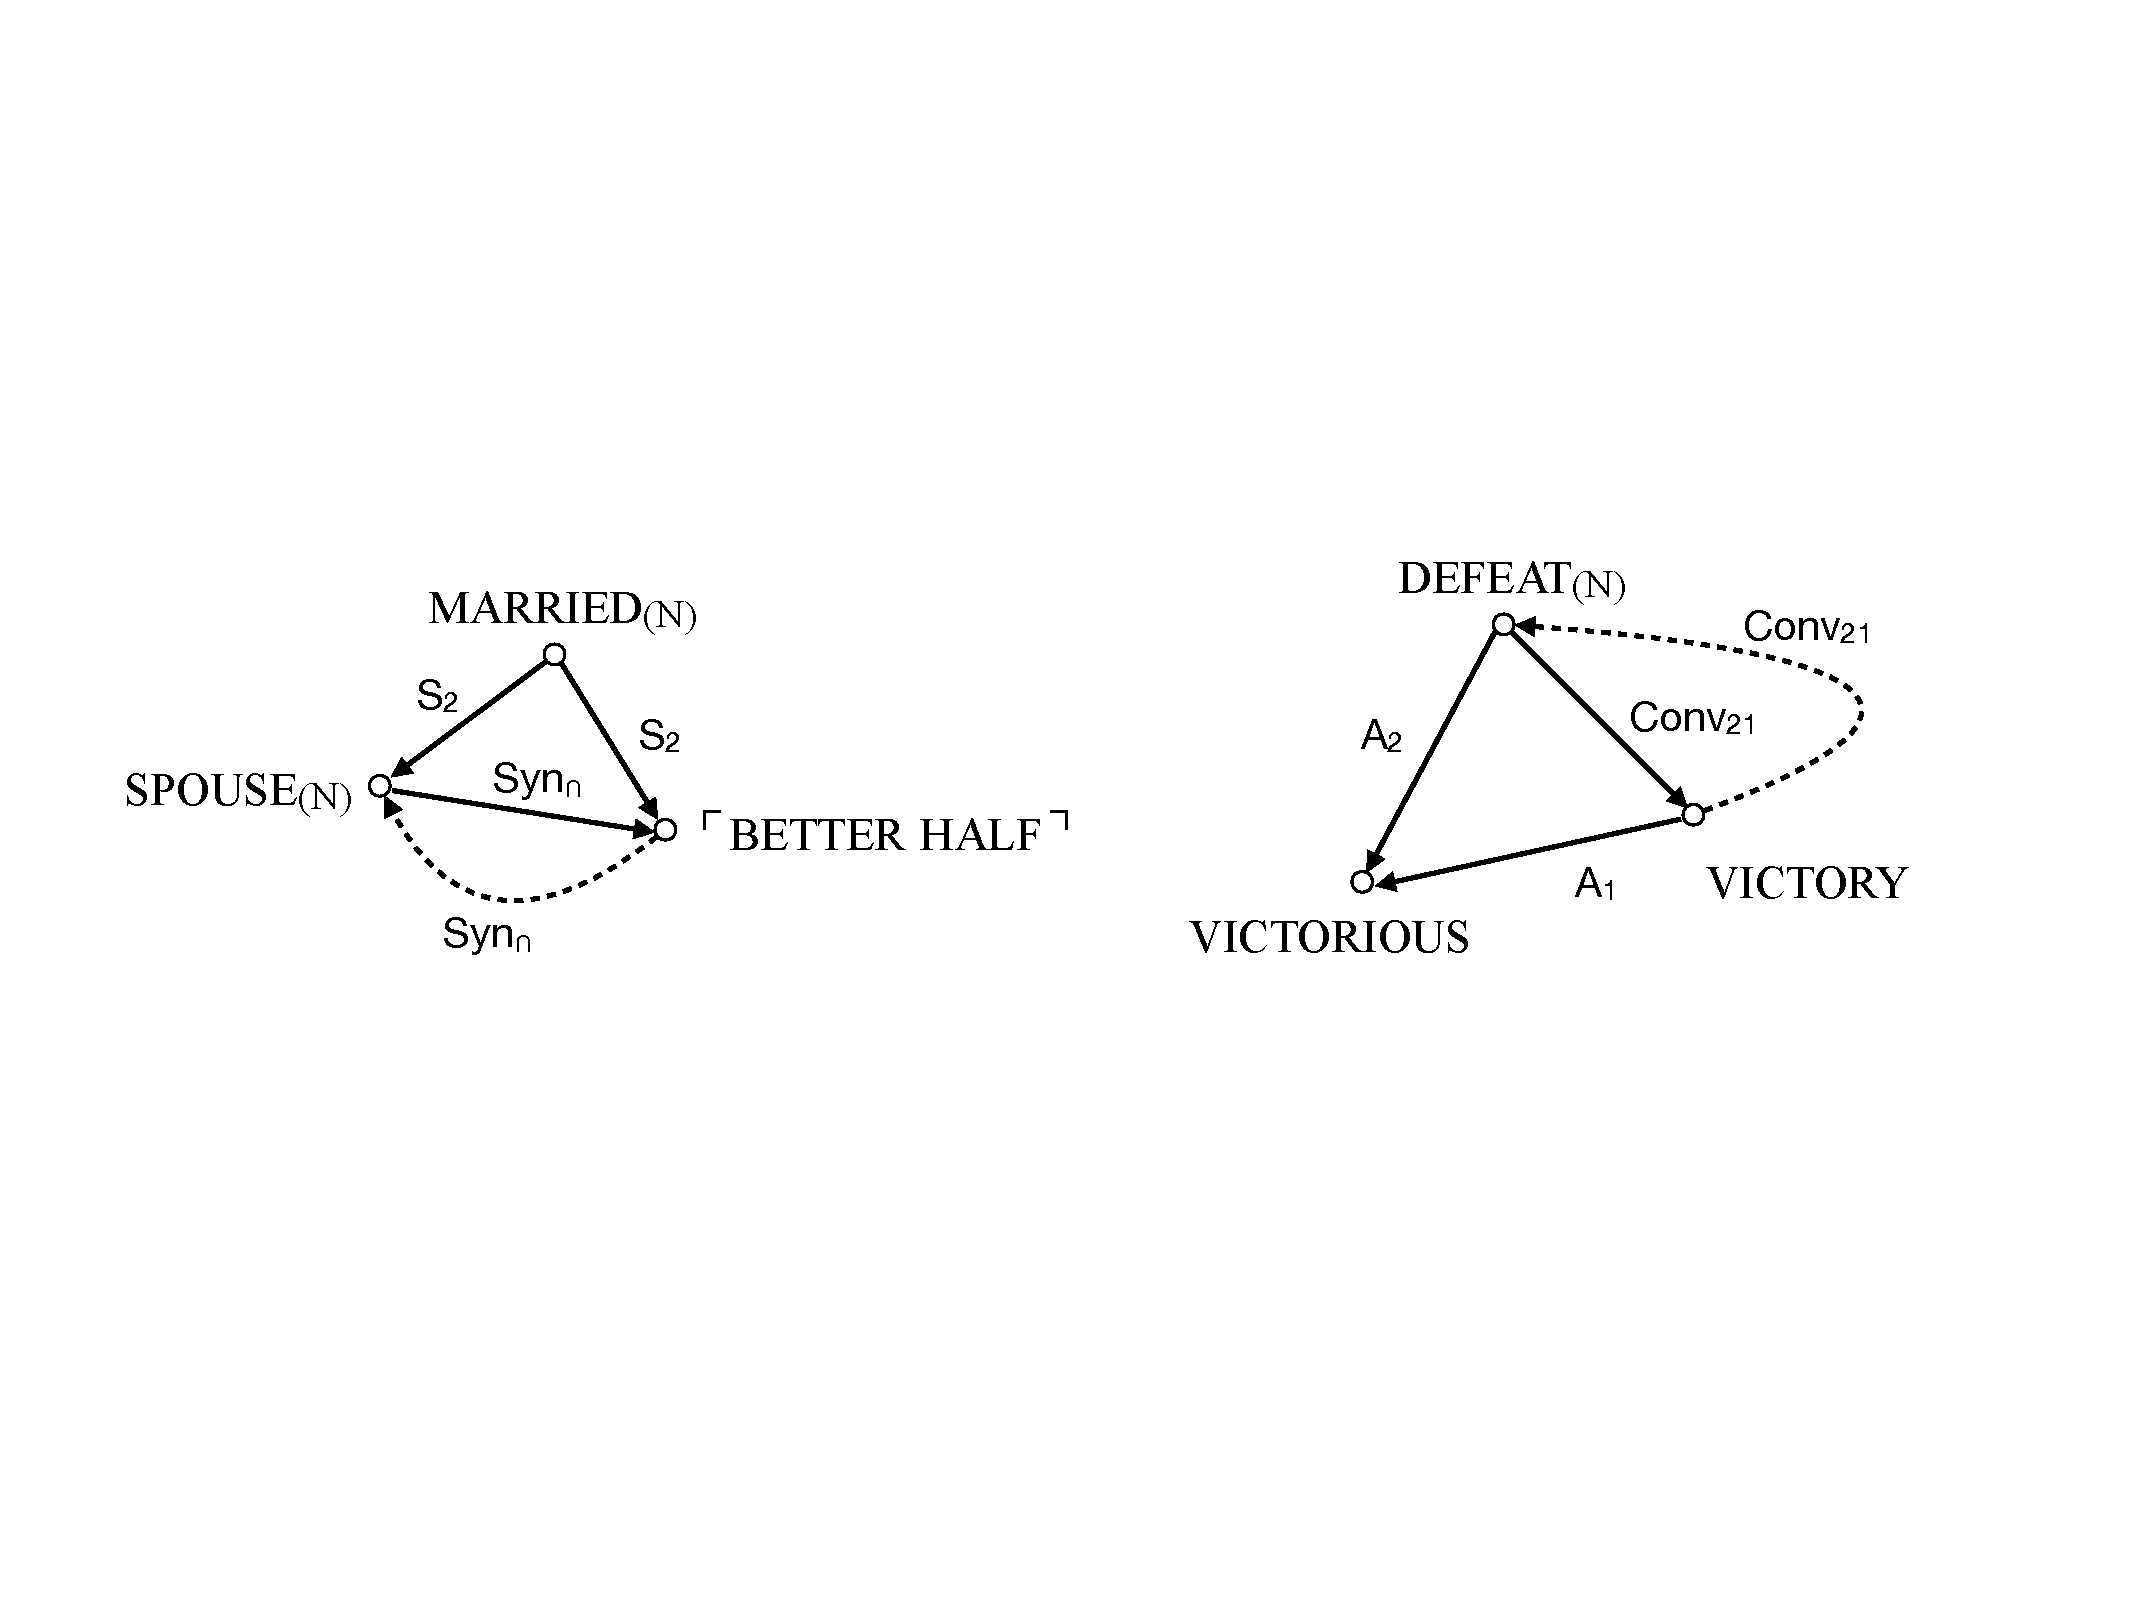
\includegraphics[width=0.9\linewidth]{Fig/LexicalNetworks/LFClusters.pdf}
\caption{Two LF-based lexical clusters}\label{fig:LFClusters}
\end{figure}

In \figref{fig:LFClusters}, solid arrows correspond to illustrations given in \ref{ex:clusteringInfRule1} and \ref{ex:clusteringInfRule2}; dashed arrows are additional clustering LF relations.

\subsubsection{Lexical vs. topological proximity}\label{sec:lexicalProximityTopologicalProximity}

Formal properties presented above show that $\mathcal{G}_{LS}$s are not \notion{random graphs}\index[notion]{graph!random \tld}\index[notion]{random graph}, i.e., graphs in which nodes and connecting arcs are randomly distributed.\footnote{In mathematical\slashs{}statistical terms, a random graph is a graph in which the distribution of node degrees follows a Poisson law; by contrast, the degree distribution of a small-world graph follows a power law \parencite[849]{Gaume2008}.} They are structured as small-world networks, whose topological properties can be exploited to access, study, and reason on the information they encode. The main advantage of small-world lexical networks over the better-known lexical taxonomies\index[notion]{taxonomy}\index[notion]{lexical network!taxonomic \tld} (\sectref{sec:shapeOfLexicons}, p.\thinspace\pageref{sec:shapeOfLexicons}) is that they do not adhere to one primary classifying\slashs{}hierarchization principle; consequently, they allow for very flexible and varied types of computation.

To illustrate the computability of small-world networks, we focus here on \notion{lexical proximity}\index[notion]{proximity, lexical} (whether semantic or combinatorial) that can be inferred from the topology of $\mathcal{G}_{LS}$s\index[notion]{graph!topology of a \tld}\index[notion]{topology}. This is well illustrated in visualizations\index[notion]{visualization} performed by the Spiderlex\index[notion]{Spiderlex} graph browser\index[notion]{network \lfgp{see also \textit{graph}}!\tld\ browser} (cf. \sectref{sec:LFRelationsBackboneOfLFs}, ``Visualization of Lexical Systems,'' p.\thinspace\pageref{rem:visualizationLS}), where clusters of lexical entities\index[notion]{cluster of nodes in a graph}\index[notion]{node of a network\slashs{}graph!cluster of \tlds} are identified by a stochastic algorithm that computes \notion{topological proximity}\index[notion]{topology!topological proximity} between lexical nodes \parencite{Gaume2004,Gaume2008}. This proximity is visually represented by two means: 

\begin{itemize}

\item the geometric distribution of nodes in the visualization\index[notion]{node of a network\slashs{}graph!geometric distribution of \tlds}\index[notion]{geometric distribution of graph nodes} -- the closer the nodes from the viewpoint of the graph topology, the closer they are positioned;

\item the color coding of node clusters identified by the topological analysis -- these clusters correspond to semantic-combinatorial classes of lexical entities.

\end{itemize}

\paragraph*{Lexical spaces.}\label{par:lexicalSpaces}

We have established earlier that $\mathcal{G}_{LS}$s possess a high clustering rate\index[notion]{cluster of nodes in a graph!clustering rate}\index[notion]{graph!clustering rate of a \tld} (\sectref{sec:basicsGraphTheory}, p.\thinspace\pageref{par:highClusteringRate}): at the microscopic level\index[notion]{microscopic structure (of a graph)}, their nodes tend to form small clusters of lexical entities that are mutually interrelated. Such clusters are of course identified by the topological analysis of a $\mathcal{G}_{LS}$. However, at the macroscopic level\index[notion]{macroscopic structure (of a graph)}\index[notion]{graph!microscopic vs. macroscopic structure of a \tld}, broader clusters are also identified; they bring together lexical entities that are more loosely related but form a distinct semantic-combinatorial \notion{lexical space}\index[notion]{lexical space} in the graph and, hopefully, in the Mental Lexicon\index[notion]{Mental Lexicon} this graph encodes.

\figref{fig:proxemyCIGARETTE}\phantomsection\label{txt:lexicalProximityCIGARETTE} below serves to illustrate the notion of lexical space and, more broadly, the outcome of a $\mathcal{G}_{LS}$'s topological analysis. It shows:

\begin{itemize}

\item lexical proximity identified by means of a topological analysis of the fr-LN\index[notion]{lexical network!French \tld\ [fr-LN]}\index[notion]{lexical database!French Lexical Network [fr-LN]};

\item visualization means used by Spiderlex to represent lexical spaces.

\end{itemize}

In this illustration, lexical proximity is  computed on the polysemy structure\index[notion]{polysemy!\tld\ structure of a vocable}\index[notion]{vocable!polysemy structure of a \tld} of the French vocable \textsc{cigarette}, which has been explained in \sectref{sec:non-LFRelationsInLSs} (p.\thinspace\pageref{txt:CIGARETTE}). To work on the complete polysemy of \textsc{cigarette}, three topological explorations are performed as so-called \textit{random walks} \parencite[Sec.~3]{Gaume2008}: one for each sense of the vocable taken as point of origine of the random walk. The three lexical nodes that are origines of random walks appear in \figref{fig:proxemyCIGARETTE} as triangles, rather than discs.

\begin{figure}

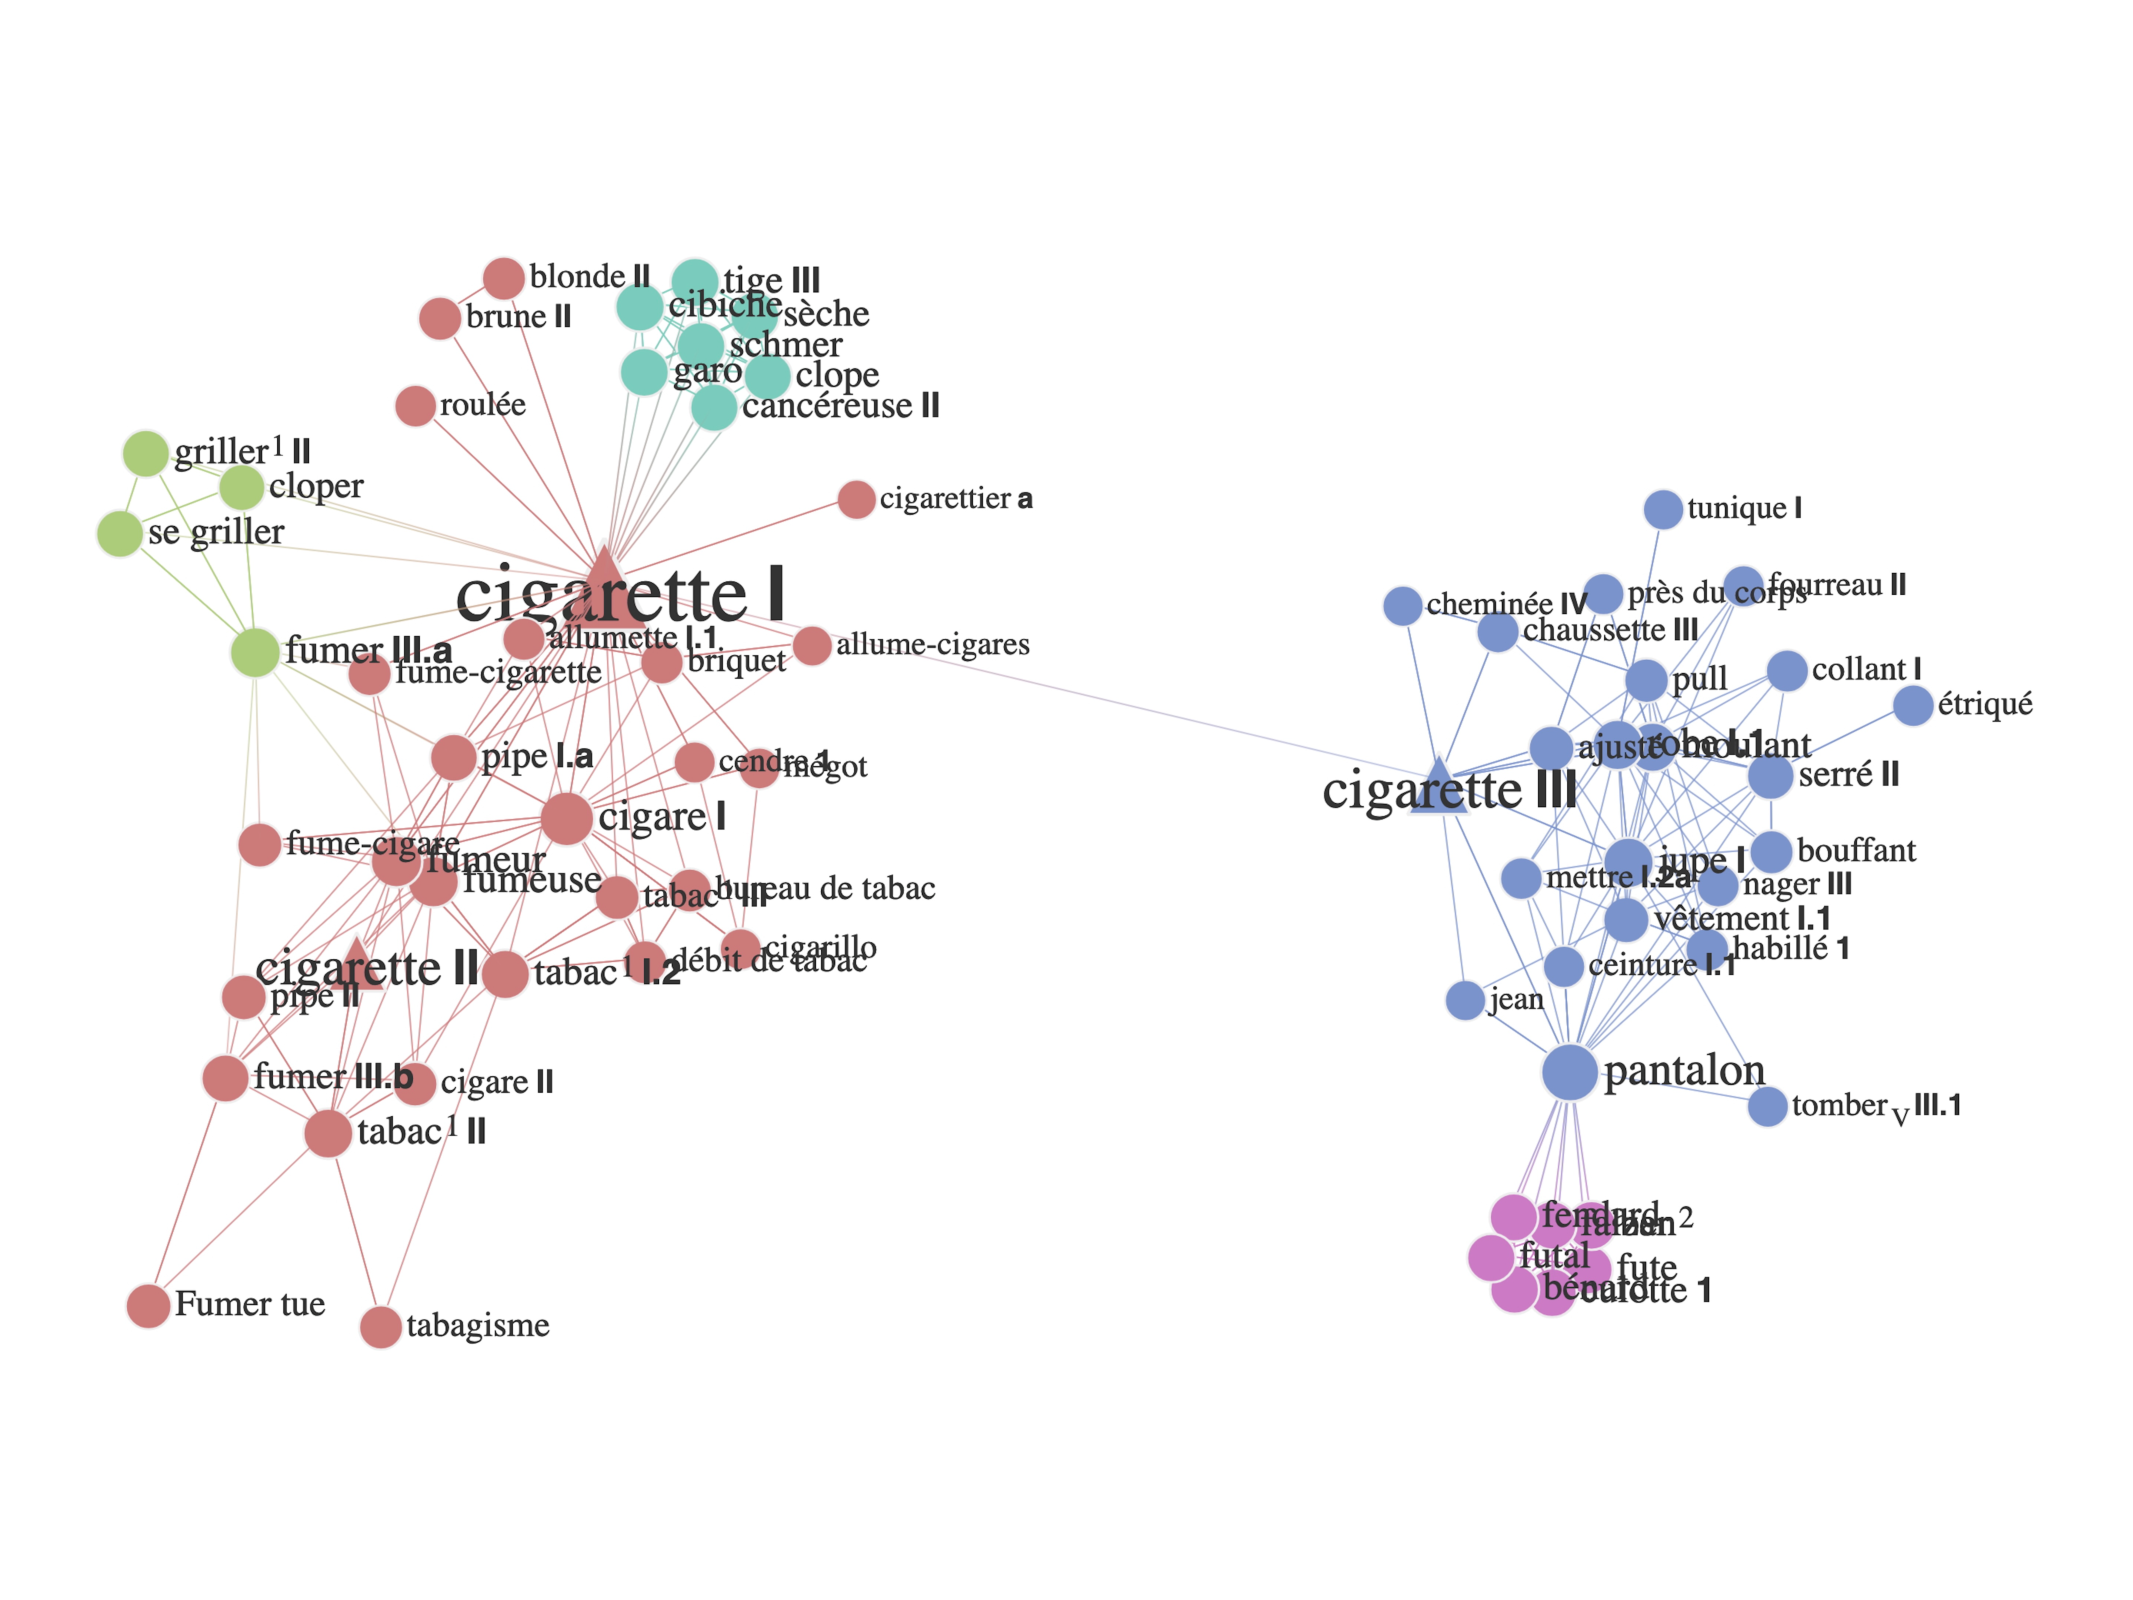
\includegraphics[width=\linewidth]{Fig/LexicalNetworks/proxemyCIGARETTE.pdf}
\caption{Lexical proximity computed on the polysemy of {\smaller French}~\textsc{cigarette} in the fr-LN}\label{fig:proxemyCIGARETTE}
\end{figure}

Let us make two comments on \figref{fig:proxemyCIGARETTE} in order to illustrate the linguistic relevance of the topological analysis and geometrization algorithms that have lead to this visualization.

First, the basic lexical unit\index[notion]{basic lexical unit of a vocable}\index[notion]{vocable!basic lexical unit of a \tld} \textsc{cigarette}\sensenum{I} and the metonymic\index[notion]{metonymy} sense \textsc{cigarette}\sensenum{II} `habit of smoking \textit{cigarettes}\sensenum{I}' form together a single lexical space, while the met\-aphoric\index[notion]{metaphor} sense \textsc{cigarette}\sensenum{III} `\lfgp{piece of clothing X} long and tight against the body, \idiom{as if} it had the shape of a \textit{cigarette}\sensenum{I}' is singled out, at the center of its own lexical space. These two spaces are located far apart, their connection holding by only one thread: the metaphor copolysemy\index[notion]{polysemy!co\tld}\index[notion]{copolysemy!\tld\ relation of metaphor} relation between \textsc{cigarette}\sensenum{I} and \textsc{cigarette}\sensenum{III}. This reflects the fact that a metonymy belongs to the same broad conceptual domain as its source, while a metaphor can totally escape the gravitation field, so to speak, of the copolyseme it originates from.

Second, the two lexical spaces identified above are themselves constituted of clusters that display their own lexical cohesion. Such is the case, in the lexical space of \textsc{cigarette}\sensenum{I} and \textsc{cigarette}\sensenum{II} combined, of the small cluster constituted of \textsc{fumer}\sensenum{III} `smoke\tsub{(V)}' -- that is \lfappl{Real\tsub{1}}{\textit{cigarette}\sensenum{I}} -- and three of its synonyms: \textsc{cloper}, \lu{griller}{}{1}{II} and \textsc{se~griller} (see top left corner of \figref{fig:proxemyCIGARETTE}). This is an extremely tight cluster -- and it is geometrically displayed as such -- for two linguistic reasons: (i)~the lexical units it contains are all values of \lf{Syn} for each other\footnote{Such cluster is called a \textit{clique}: a (sub)graph where every two nodes are connected.}\index[notion]{clique} and (ii)~they are additionally all values of the same LF application \lfappl{Real\tsub{1}}{\textit{cigarette}\sensenum{I}}.

\begin{furtherreading}
On the Lexical System approach to the modeling of polysemy, see \textcite{Polguere2018c}; on small-world lexical networks in lexicology\index[notion]{lexicology}\slashs{}lexicography\index[notion]{lexicography}, see \textcite{LoiseauEtAl2010,Polguere2014c-e,Polguere2016b-e}; in psycholinguistics\index[notion]{psycholinguistics}, see \textcite{GaumeEtAl2002,GaumeEtAl2008,DeDeyneEtAl2017}; in Natural Language Processing\index[notion]{Natural Language Processing}, see \textcite{Biemann2012}.
\end{furtherreading}

\section{Proof of concept: the French Lexical Network [fr-LN]}\label{sec:fr-LN}

In lieu of conclusion, we present briefly the lexicographic enterprise that produced the first large-scale Lexical System: the \notion{French Lexical Network} \mbox{[\notion{fr-LN}]}\index[notion]{French Lexical Network [fr-LN]|emph}\index[notion]{lexical database!French Lexical Network [fr-LN]|emph}\index[notion]{lexical network!French \tld\ [fr-LN]|emph}\index[notion]{lexical network!lexicography of \tlds}\index[notion]{lexicography!\tld\ of lexical networks}. Bibliographic references on important aspects of the fr-LN project are provided at the end of the section.

\subsection{Organization and progression of the fr-LN project}

The construction of the fr-LN is an ongoing long-term endeavor that started at the ATILF CNRS laboratory (Nancy, France) in 2011. An initial four-year funded project (called \textit{RELIEF}, see \cite{LuxPogodallaPolguere2011}) achieved the following tasks:

\begin{enumerate}

\item[1.a)] training of a team of lexicographers in the theory and practice of Explanatory Combinatorial Lexicology\slashs{}Lexicography\index[notion]{Explanatory Combinatorial!\tld\ Lexicology}\index[notion]{lexicology!Explanatory Combinatorial \tld}\index[notion]{Explanatory Combinatorial!computational \tld\ Lexicography}\index[notion]{lexicography!computational Explanatory Combinatorial \tld};

\item[1.b)] implementation -- in parallel with 1.a -- of a lexicographic editor\index[notion]{editor, lexicographic}\index[notion]{lexicography!lexicographic editor} tailor-made for the lexicography of Lexical Systems, whose capabilities were gradually incremented as the project proceeded with lexicographic description \parencite{GaderEtAl2012};

\item[2)] construction of a nucleus fr-LN for a core French vocabulary of around 3,700 vocables;

\item[3)] standard lexicographic work proceeding by important semantic fields (feelings, geographical elements, animals, ...).

\end{enumerate}

This initial stage of the project resulted in a Lexical System that modeled a significant sample of the French lexicon and that later expanded into a full-fledged small-world network\index[notion]{network \lfgp{see also \textit{graph}}!small-world \tld}\index[notion]{small-world!\tld\ network} (as defined in \sectref{sec:formalPropertiesLS}, p.\thinspace\pageref{sec:formalPropertiesLS}).

The fr-LN is in constant evolution both in terms of the number of lexical entities it describes and in terms of depth\slashs{}accuracy of the description. At the time of writing, its coverage can be quantified as follows:

\begin{center}
\setlength{\tabcolsep}{2.2pt}
%\setlength\extrarowheight{1.2pt}
\begin{tabular}{ l c r }

\textsf{\textbf{Lexical entities, i.e., network nodes}} & \textsf{\textbf{:}} & \textsf{\textbf{30,180}} \\
Vocables, i.e., lexicographic entries & : & 19,084 \\
Polysemy rate [= Lexical entities\slashs{}Vocables] & : & 1.58 \\[+6pt]

\textsf{\textbf{Lexical relations, i.e., network arcs}} & \textsf{\textbf{:}} & \textsf{\textbf{85,941}} \\
LF relations & : & 67,478 \\
Copolysemy relations & : & 9,960 \\
Idiom-component relations & : & 8,171 \\
Meaning-inclusion relations & : & 332 \\

\end{tabular}
\end{center}

The above statistics show that the current fr-LN is a lexical network of significant proportions: approximately 30,000 lexical nodes for 85,900 lexical relations. In accordance with the properties of Lexical Systems (cf. \sectref{sec:LFRelationsBackboneOfLFs}, p.\thinspace\pageref{sec:LFRelationsBackboneOfLFs}), LF relations form the bulk of the relational structure of the model. Meaning-inclusion relations are underrepresented as the work on the writing of lexicographic definitions is still at an embryonic stage.

In the absence of a dedicated lexicographic team, the fr-LN now evolves mainly on demand, according to the needs of researchers, language teachers, etc. who are collaborators on the project or are making use of the resource. The fr-LN's lexicographic data is available in open access, to be used for Natural Language Processing\index[notion]{Natural Language Processing} or computational linguistic work -- see \textcite{ATILF2024a}, for the network itself, and \textcite{ATILF2024b}, for the distribution of lexicographic examples\index[notion]{example, lexicographic} embedded in the fr-LN.

\subsection{New lexicography of lexical networks}\label{sec:lexicographyOfLNs}\index[notion]{lexicography!\tld\ of lexical networks|emph}\index[notion]{lexical network!lexicography of \tlds|emph}

The fr-LN project is mature enough -- in terms of coverage and applications it has generated -- to be seen as a proof of concept for Lexical Systems as plausible models of the Mental Lexicon. It demonstrates that network lexical models primarily structured by standard LF relations can offer new insights into the organization of lexical knowledge and, very importantly, that such models can indeed be lexicographically built.

As regards this last point, it is essential to stress the importance of the technological aspects of this new lexicography of lexical networks. Modern physics or astronomy could not exist without advanced technological means (cyclotrons, orbiting telescopes, etc.); similarly, though at a much more modest level, the lexicography of lexical networks has been made possible by the development of a sophisticated editor\index[notion]{editor, lexicographic}\index[notion]{lexicography!lexicographic editor} that allows lexicographers to literally jump from one lexical entity to another, encoding lexical relations while simultaneously creating new lexical nodes in the process, if the targeted lexical entity is not already present in the network.\footnote{We do not illustrate the use of the Lexical System lexicographic editor (named \textit{Dicet}, see \cite{GaderEtAl2012}) as a next generation editor (\textit{ItsyBitsy}) is under development at the time of writing.} This \emph{lexicographic gesture} \parencite{Polguere2012e-e} ensures that lexical entries always point to (the lexical entry of) actual lexical entities and forces lexicographers to encode a lexical relation as a link between two lexical entities that are (at least, minimally) modeled in the lexical network.

Anyone who has extensively used standard dictionaries (for language teaching, translation, etc.) knows that this is far from being the case in such models. The system of lexical relations present in a standard dictionary -- that has been termed the dictionary's \notion{mediostructure}\index[notion]{dictionary!mediostructure of a \tld}\index[notion]{mediostructure (of a dictionary)}\phantomsection\label{txt:mediostructure} \parencite{Wiegand1996,GouwsPrinsloo1998} -- is only modeled by cross-references in the text of the \notion{microstructure}\index[notion]{dictionary!microstructure of a \tld}\index[notion]{microstructure (of a dictionary)}. At the scale of the whole lexicon, however, this cross-referencing is necessarily approximate for logistic reasons. Only by building a lexical model that \emph{is}, so to speak, a mediostructure (i.e., a lexical network) can one ensure that the modeling of lexical relations -- the essence of the lexicon's structure (cf. Postulate~1, \sectref{sec:shapeOfLexicons}, p.\thinspace\pageref{txt:postulateStrucLexicons}) -- is truly valid and unambigous.

Finally, essential technology includes visualization and navigation tools such as Spiderlex\index[notion]{Spiderlex}\index[notion]{visualization} (extensively used to produce illustrations in the present chapter). Their purpose is threefold: improve access to the content of Lexical Systems, visualize complex topological information and help lexicographers diagnose missing or wrongly encoded information.

\begin{furtherreading}
On the strategy adopted to organize the fr-LN's initial growth based on the encoding of standard paradigmatic LF relations that are central in the system of LFs\index[notion]{lexical function!central \tld\ (in the system of standard \tlds)},\footnotemark\ see \textcite{LuxPogodallaPolguere2011} and \textcite{PolguereSikora2013a-e}; on the small-world structure of the fr-LN, see \textcite{GaderEtAl2014a-e}; on the implementation of analogical reasoning\index[notion]{analogical reasoning} in the fr-LN, see \textcite{Ollinger2014-e}; on lexicographic edition of Lexical Systems\index[notion]{editor, lexicographic}\index[notion]{lexicography!lexicographic editor}, see \textcite{GaderEtAl2012} and \textcite{Polguere2012e-e}; on the modeling of terminologies\index[notion]{terminology} within general language Lexical Systems, see \textcite{GotkovaEtAl2024}.
\end{furtherreading}\footnotetext{Roughly, those paradigmatic LFs whose ID is boxed in the table presenting the ``System of standard simple lexical functions'' (\chapref{chap:NotionLF}, p.\thinspace\pageref{tab:systFL}).}


\clearpage{\pagestyle{empty}\cleardoublepage}
